\documentclass[11pt, a4paper]{memoir}
% extrafontsizes
\usepackage{mdwlist}
%\usepackage{microtype}
\usepackage{textcomp}
\usepackage{xspace} 
\usepackage{booktabs} 
\usepackage{algorithmic}

%\usepackage{caption}
%for landscape tables
\usepackage{rotating}


\settrimmedsize{11in}{210mm}{*} 
\setlength{\trimtop}{0pt} 
\setlength{\trimedge}{\stockwidth} 
\addtolength{\trimedge}{-\paperwidth} 
\settypeblocksize{7.75in}{33pc}{*} 
\setulmargins{4cm}{*}{*} 
\setlrmargins{1.6in}{*}{*} 
\setmarginnotes{17pt}{51pt}{\onelineskip} 
\setheadfoot{\onelineskip}{2\onelineskip} 
\setheaderspaces{*}{2\onelineskip}{*} 
\checkandfixthelayout
\fixpdflayout

\nouppercaseheads

\makechapterstyle{abstr}{%
  \chapterstyle{default}
  \renewcommand*{\chapnumfont}{\normalfont\Large}
  \renewcommand*{\chaptitlefont}{\normalfont\Large}
 \settowidth{\chapindent}{\chapnumfont 111}
\renewcommand*{\printchaptertitle}[1]{%
\vskip\onelineskip
\raggedleft {\chaptitlefont ##1\vspace*{2\onelineskip}}\par\nobreak}
}    

\makechapterstyle{conten}{%
  \chapterstyle{default}
  \renewcommand*{\chapnumfont}{\normalfont\HUGE}
  \renewcommand*{\chaptitlefont}{\normalfont\HUGE}
 % \settowidth{\chapindent}{\chapnumfont 111}
%\renewcommand*{\printchaptertitle}[1]{%
%   \vskip\onelineskip
%    \raggedleft {\chaptitlefont ##1\vspace*{2\onelineskip}}\par\nobreak}
}    

\makechapterstyle{ell2}{%
  \chapterstyle{default}
  \renewcommand*{\chapnumfont}{\normalfont\HUGE}
  \renewcommand*{\chaptitlefont}{\normalfont\HUGE}
  \settowidth{\chapindent}{\chapnumfont 111}
  \renewcommand*{\chapterheadstart}{\begingroup
    \vspace*{\beforechapskip}%
    \begin{adjustwidth}{}{-\chapindent}%
    \hrulefill
    \smash{\rule{2.6pt}{25mm}}
    \end{adjustwidth}\endgroup}
  \renewcommand*{\printchaptername}{}
  \renewcommand*{\chapternamenum}{}
  \renewcommand*{\printchapternum}{%
    \begin{adjustwidth}{}{-\chapindent}
    \hfill
    \raisebox{10mm}[1pt][0pt]{\chapnumfont  \thechapter}%
                              \hspace*{1.5em}
    \end{adjustwidth}\vspace*{2\onelineskip}}
    
  \renewcommand*{\printchaptertitle}[1]{%
   \vskip\onelineskip

    \raggedleft {\vspace*{-3\onelineskip}\chaptitlefont ##1\vspace*{2\onelineskip}}\par\nobreak}}                             



%used for a bib after each chapter                                    
\usepackage[sectionbib]{natbib}
\usepackage{chapterbib}

\usepackage[ansinew]{inputenc}
\usepackage[T1]{fontenc}
\usepackage{amssymb}
\usepackage{amsmath}
\usepackage{amsfonts}
\usepackage{relsize}
\usepackage{guit}
\usepackage{fancyvrb}
\usepackage{calc}
\usepackage{texnames}
\usepackage{placeins}

\usepackage{nicefrac}


\usepackage[english]{babel}
\usepackage[english]{varioref}

\setcounter{tocdepth}{2}
\usepackage{hyperref}
\usepackage{multicol}
\usepackage{setspace}

\usepackage[small]{caption}


%\setstocksize{11in}{8.5in}
%\settrimmedsize{11in}{8.5in}{*}
%\settrims{0in}{0in}
%\settypeblocksize{9.0in}{30pc}{*}
%\setlrmargins{1.25in}{*}{*}
%\setulmargins{1.0in}{*}{*}
%\setheadfoot{13pt}{26pt}
%\setheaderspaces{*}{13pt}{*}
\checkandfixthelayout
\openright

%\usepackage[T1]{fontenc}

%\font\warnock="Georgia" at 11pt

%\renewcommand{\rmdefault}{ptm}
%\renewcommand{\rmdefault}{warnock}
%\usepackage{fontspec}
%\setromanfont{Georgia}


%Compensating for On-Body
%Placement Effects in Wearable Sensors

%\usepackage{comment}
\usepackage[english]{babel}
\usepackage{graphicx}


\usepackage{multirow}
%\usepackage{isorot}%\usepackage[dvips]{graphicx}
%\addtolength{\tabcolsep}{3pt}
\usepackage{subfig}

\DeclareGraphicsExtensions{.pdf,.jpg,.png}
\graphicspath{{OnOff/}{Displacement/}{Orientation/}{Onbody/}{Motivation/}{Conclusion/}}

%\ttfgeorgia

\usepackage{subfig}
\usepackage{tabulary}

\IfFileExists{lmodern.sty}{%
  \RequirePackage{lmodern}
  \usepackage[T1]{fontenc}}{}
  \IfFileExists{mathpazo.sty}
             {\RequirePackage[sc]{mathpazo}}
             {\renewcommand\rmdefault{ppl}}
%\usepackage{titlepages}  % code of the example titlepages
%\usepackage{memlays}     % extra layout diagrams
%\usepackage{dpfloat}     % floats on facing pages
%\usepackage{fonttable}[2009/04/01] 

%\settocdepth{subsection}
%%% Numbering down to subsections as well
%\setsecnumdepth{subsection}

% end demo

%nice package to make referencing easier
%no longer the need for Table~\ref{somelabel}
%just use \cref{somelabel}
%\usepackage{cleveref}

%\newcommand{\mycaption}[2][\@empty]{ 
%\captionnamefont{\sffamily\hfill} \captiondelim{\hfill} \captionstyle{\centerlastline\\}
%\captiontitlefont{\scshape} \setlength{\belowcaptionskip}{10pt} \ifx \@empty#1 \caption{#2}\else \caption[#1]{#2}}



\fixpdflayout
\begin{document}

\makepagestyle{ruled2} 

%\makeevenfootruled{\thepage}{}{} % page numbers at the outside 
\makeoddfoot{ruled2}{}{}{\thepage} 
\makeevenfoot{ruled2}{\thepage}{}{} 
\makeheadrule{ruled2}{\textwidth}{\normalrulethickness} 
\makeevenhead{ruled2}{\leftmark}{}{} % small caps 
\makeoddhead{ruled2}{}{}{\rightmark}

\makepsmarks{ruled2}{% 
 \nouppercaseheads 

\createmark{chapter}{left}{shownumber}{}{. \space} 
\createmark{section}{right}{shownumber}{}{. \space} 
\createplainmark{toc}{both}{\contentsname} 
\createplainmark{lof}{both}{\listfigurename} 
\createplainmark{lot}{both}{\listtablename} 
\createplainmark{bib}{both}{\bibname} 
\createplainmark{index}{both}{\indexname} 
\createplainmark{glossary}{both}{\glossaryname}
}

\makepagestyle{companion2} 
\makerunningwidth{companion2}{\textwidth}
\makeheadrule{companion2}{\textwidth}{\normalrulethickness}
\makeheadposition{companion2}{flushright}{flushleft}{}{}
\makeevenhead{ruled2}{\leftmark}{}{} % small caps 
\makeoddhead{ruled2}{}{}{\rightmark}

\makepsmarks{companion2}{% 
\nouppercaseheads 
\createmark{chapter}{both}{nonumber}{}{} 
\createmark{section}{right}{shownumber}{}{. \space} 
\createplainmark{toc}{both}{\contentsname} 
\createplainmark{lof}{both}{\listfigurename} 
\createplainmark{lot}{both}{\listtablename} 
\createplainmark{bib}{both}{\bibname} 
\createplainmark{index}{both}{\indexname} 
\createplainmark{glossary}{both}{\glossaryname}
}


\fixpdflayout
\frontmatter
%\pagestyle{headings}

\pagestyle{empty}
% title page
%\vspace*{\fill}
\begin{flushleft}
\medskip 
\medskip 
\HUGE\textrm{Compensating for On-Body Placement Effects in Activity Recognition}\par
%\HUGE\textrm{Sensor Placement Tolerance in Activity Recognition}\par
\end{flushleft}
\medskip
\begin{flushright}
%\LARGE
{Kai Kunze}\par
\end{flushright}
\vspace*{290pt}
%\normalsize\textsf{Maintained by Lars Madsen}\par
%\end{center}%
%\vspace*{\fill}
%\begin{center}
\begin{flushleft}\par
\textrm{This dissertation has been submitted to the}\par
%\end{flush}
%\begin{flushleft}
%\LARGE
\textrm{Universit\"at Passau}\par
%\LARGE
\textrm{Fakult\"at f\"ur Informatik und Mathematik}\par
Thesis Advisor: Prof. Dr. Paul Lukowicz \par
Co-Advisor: Prof. Dr. Hans Gellersen
%\end{center}
\end{flushleft}
\vspace*{\fill}
%\def\THP{T\kern-0.2em H\kern-0.4em P}%   OK for CMR
%\def\THP{T\kern-0.15em H\kern-0.3em P}%   OK for Palatino
%\newcommand*{\THPress}{The Herries Press}%
\begin{flushright}
June 2011
%\settowidth{\droptitle}{\textsf{\THPress}}%
%\textrm{\normalsize \THP} \\
%\textsf{\THPress} \\[0.2\baselineskip]
%\setlength{\droptitle}{0pt}%
\end{flushright}
\clearpage
%\setupshorttoc
%\tableofcontents
%\clearpage
%\setupparasubsecs
%\setupmaintoc
%\pagenumbering{arabic}
\chapterstyle{abstr}
\pagestyle{empty}
% title page
\vspace*{240pt}
%\begin{flushright}
%to my mother
%\end{flushright}
\newpage
\clearpage
\begin{flushleft}
\medskip
\Large\textrm{Acknowledgments}
\medskip
\end{flushleft}
My sincere gratitude goes to Paul Lukowicz, my thesis advisor,
who is often on a tight schedule. Yet, he always makes time to provide valuable research input and inspiration.
I can always rely on his support and vast experience.

Additionally, I would like to give a warm thank you to Hans Gellersen. I'm proud to have him as second advisor, he's an extraordinary researcher and I valued his input and help throughout my Ph.D. studies.

Thanks to David Bannach, Gernot Bahle, Josef Neuburger, Gerald Pirkl, Jens Weppner and Kamil Kloch, for being great peers, for critic and proofreading, Georg Ogris, Tobias Franke, Jinyuan Cheng, Agnes Gr\"unerbl,  Michael Barry, Karl Stockinger and Peter Barth for being outstanding colleagues and for sparking interesting discussions.

Special thanks go to Ian Cloete, Christoph Schuba, Helmut Stadm\"uller and Ernst Heinz, all exceptional and inspiring teachers. Without their guidance, I would definitely not work in research today.

Thanks to Thad Starner, Albrecht Schmidt and Michael Beigl for giving valuable advice and sharing their expertise.
Other friends and inspiring colleagues, I want to thank: Oliver Amft, Ulf Blanke, Todd Farrell, Martin Kurserow, Till Riedel, Michael Springmann, Kristof Van Laerhoven and Jamie Ward.

Cyrille Thouvenin, Roland Westrelin, Eric Lemoine and Nicolas Fugier  thanks for an amazing time in Grenoble.

Kurt Partridge, Bo Begole, Rowan Nairn and Max Van Kleek thank you for a great summer at PARC.

Holger, Melanie, Sanjit and Julia deserve also a thank you for their close friendship and for putting up with me over the last couple of years.

Most importantly, I sincerely thank Renate Kunze, my mother, and Anita and Helmut Woll, my grandparents, 
for their love and support. No matter what, I can always count on them. Without them this work would not have been possible.
\newline
\newline
\newline
\newline
\newline
\noindent Kai Kunze \newline
\noindent Passau, 2011

\begin{flushleft}
\medskip
\Large\textrm{Abstract}
\medskip
\end{flushleft}This thesis investigates, how placement variations of electronic devices influence the possibility of using sensors integrated in those devices for context recognition.
The vast majority of context recognition research assumes well defined, fixed sensor locations.
%This is only acceptable for very narrow application domains, e.g. in an industrial setting.
%To reach a more wide spread adoption of activity recognition applications, we can utilize 
 %user-owned, mobile appliances (for details see~\ref{mot:sota}). Most of them come already equipped with sensors.
Although this might be acceptable for some application domains (e.g. in an industrial setting), users, in general, will have a hard time coping with these limitations. If one needs to remember to carry dedicated sensors and to adjust their orientation from time to time, the activity recognition system is more distracting than helpful. How can we deal with device location and orientation changes to make context sensing mainstream?
%to assist users during everyday tasks using mobile appliances that are already equipped with sensors.
%For a more widespread adoption, activity recognition can leverage this sensor penetration
%Some research already utilizes the sensors embedded in many of todays mobile appliances.
%Today, many mobile appliances are already equipped with sensors.
%Sensor encapsulation into clothing has been demonstrated.
%This substrate can be used for a wide spread adoption of activity recognition (for detailed related work see~\ref{}).
%It is thus often taken for granted that users can be easily equipped with sensors in every day situations. 
%However, the users cannot be expected to reliably 
%and firmly fix these sensors to narrowly defined on-body locations.
%However, this does not imply that the user can be expected to reliably 
%and firmly fix the sensors to narrowly defined on-body locations.
%Traditional context and activity recognition research mostly uses dedicated
%sensors with known location and orientation.
%In general, the quality of these embedded sensors
%is not much different from the devices typically used in dedicated wearable sensing systems.
%This high level of sensor penetration presents a unique chance for activity recognition.
%Only few related work exists dealing with this issue (for details see~\ref{}).
This thesis presents a systematic evaluation of device placement effects in context recognition.
We first deal with detecting if a device is carried on the body
or placed somewhere in the environment. If the device is placed on the body, it is useful to know on which body part.
We also address how to deal with sensors changing their position and their orientation
during use. For each of these topics some highlights are given in the following.

Regarding environmental placement, we introduce an active sampling approach
to infer symbolic object location. This approach requires only simple sensors (acceleration,
sound) and no infrastructure setup. The method works for specific
placements such as "on the couch", "in the desk drawer" as well as for
general location classes, such as "closed wood compartment" or "open
iron surface". In the experimental evaluation we reach a
recognition accuracy of 90\% and above over a total of over 1200 measurements from 35
 specific locations (taken from 3 different rooms) and 12 abstract
 location classes. 
 
 To derive the coarse device placement on the body, we present 
a method solely based on rotation and acceleration signals
from the device. It works independent of the device orientation.
 The on-body placement recognition rate is around 80\%
 over 4 min. of unconstrained motion data for the worst scenario and
 up to 90\% over a 2 min. interval for the best scenario.
We use over 30 hours of motion data for the analysis.
Two special issues of device placement are orientation and displacement.
This thesis proposes a set of heuristics that significantly 
increase the robustness of motion sensor-based activity recognition 
with respect to sensor displacement. We show how, within 
certain limits and with modest quality degradation, motion sensor-based 
activity recognition can be implemented in a displacement tolerant way.
We evaluate our heuristics first on a set of synthetic lower arm
 motions which are well suited to illustrate the strengths and limits
 of our approach, then on an extended modes of locomotion problem
 (sensors on the upper leg) and finally on a set of exercises performed
 on various gym machines (sensors placed on the lower arm). 
In this example our heuristic raises the displaced recognition rate
 from 24\% for a displaced accelerometer, which had 96\% recognition
 when not displaced, to 82\%.

   

%\chapter{Abstract}
\chapterstyle{conten}
\tableofcontents*
\setlength{\unitlength}{1pt}
\clearpage
\listoffigures*
\clearpage
\listoftables*
\clearpage
%\listofegresults
%
%%%\title{Fixing Context Recognition  - Compensating for On-Body Placement Effects in Wearable Sensors} 
%%%%
\mainmatter
\chapterstyle{ell2}
\pagestyle{ruled2}
%\pagestyle{companion2}
\setsecheadstyle{\rmfamily\LARGE}
\setsubsecheadstyle{\bfseries}
\setparaheadstyle{\itshape\bfseries}
%subsection headings
%\setsubsecheadstyle{\normalfont\centering\MakeUppercase}
%\setsecheadstyle{\centering}

%\pagenumbering{arabic}

\chapter{Motivation}

\begin{flushright} 
%\textit{"Begin at the beginning and go on till you come to the end: then stop."
%\\-Lewis Carroll, Alice's Adventures in Wonderland.}\end{flushright} 
\textit{"An approximate answer to the 
right problem is worth a good deal more 
than an exact answer to an approximate problem." \\
- John Tukey}\end{flushright} 
\begingroup
\textit{Our everyday lives get more and more saturated with computing devices and embedded in them, a wide variety of sensors. With access to powerful computing, sensors and a ubiquitous Internet, why is context recognition, and with it pervasive computing, not further along and more broadly adapted? With few exceptions, most context recognition research done to date assumes dedicated sensing devices with fixed locations. These locations are often carefully chosen to suit a particular application. This is a major limitation hindering broad adoption of pervasive computing systems. Who wants to bother to put on a second "sensor suit" before leaving to work in the morning or re-adjust shifted sensors every couple of hours? Is there a way to deal with device placement and orientation changes to make context sensing more mainstream?}
%\textit{
%With people having access to powerful computing devices, the Internet being ubiquitous and pervasive computing concepts getting mainstream, why is activity sensing not further along and more broadly adapted?
%Our everyday lives get more and more saturated with computing devices and embedded sensors. Most notably, smart phones become an important computing platform and, in general, the quality of smart phone sensors is not much different from the devices typically used in dedicated wearable sensing systems. However, with few exceptions the bulk of
%context and activity recognition work done to date assumes known fixed sensor 
%locations which are often carefully chosen to suit a particular application.
%Mobile phones and other wearable devices, on the other hand, are
%carried by users in a variety of locations. In most cases they are not firmly
%fixed to the body but placed in a pocket or bag where the can shift around and have different orientations. This chapter sets the stage, exploring the state of the art in activity sensing with a focus on on-body context recognition, discussing challenges, potential obstacles.}
%This thesis presents a systematic evaluation of device
% placement effects in activity recognition. A categorization of the
% placement factors concerning context recognition systems is
% proposed. We present a systematic evaluation of these device
% placement factors on common sensing modalities,
% used in activity recognition today. In the course of
% the thesis, we introduce methods to infer the symbolic placement of a
% device and approaches to deal with coarse grain and fine variations
% in placement. This motivation chapter gives a small introduction
% into the current state of activity recognition. According to an
% assessment using two user studies, two important requirements are
% sensor integration into every day objects and device placement
% independence. As those two requirements are the basis for this
% thesis, research related to them is discussed. After the
% introduction in the field, Sections~\ref{aims},~\ref{contributions}
% and \ref{mot:overview} present the aims, contribution, outline and
% overview of this thesis in relation to the state of the art in
% research.}
%\\\\ Kunze, K.,
%Wagner, F., Kartal, E., Morales Kluge, E., and Lukowicz, P. Does
%Context Matter ? - A Quantitative Evaluation in a Real World\vskip\onelineskip
\vskip\onelineskip
\begin{adjustwidth}{}{-\chapindent}%
\hrulefill 
\end{adjustwidth}\endgroup
\vskip\onelineskip
\vskip\onelineskip 
%Pervasive computing has grown up. Today, we rely more and more on the
%ubiquity of sentient objects in our everyday life with the smart phone
%becoming an important computing
%platform~(\cite{Chronis:2009p7854,Krause:2006p1884,Ofstad:2008p7556,Choudhury:2010p5381,
% hinckley2001tms}). 
%\noindent As we use computers more and more to assist us in our daily activities, the amount
%of RAM, CPU speed etc. are no longer the limiting performance factors.
%The bottleneck becomes human attention. To overcome this limitation, pervasive
%computing tries to minimize direct user interaction. Computing systems
%are to become pro-active, inferring user intent (\cite{tea}). Context
%recognition is considered a fundamental concept in pervasive computing. 
%Activity recognition today is realized using sensors on the user's body and in
%the environment. Utilizing these sensors computer systems perceive the
%user's actions and are, therefore, able to support the user pro-actively.
%The tech industry acknowledges the pervasive computing idea and
%embraces context-aware computing as a significant
%innovation. TechCrunch - a company offering news around high-tech and
%web start-up names "Context-Aware Apps" as one of 7 most important
%technologies for 2011 and describes them as follows:
Pervasive Computing has matured. Today, we rely more and more on computing devices to help us in our daily activities, with the smart phone becoming an important platform~\cite{Chronis:2009p7854,Krause:2006p1884,Ofstad:2008p7556,Choudhury:2010p5381,hinckley2001tms}. As these devices --and with them computing-- become tighter integrated in our everyday lives, the performance bottlenecks, even on mobile platforms, are no longer RAM capacity, CPU speed etc. We use computing more and more in environments in which we cannot focus our attention completely on the device in question (e.g. during our daily commute, while waiting in a queue, during lectures/meetings). In these situations, human attention is sparse. It becomes the crucial bottleneck.

For the user to be able to interact with computer systems even in "busy" environments, 
%To levitate the user of the burden to directly interact with more and more computer systems, 
pervasive computing introduces context recognition as a core concept~\cite{tea}. 
Context recognition infers relevant information about the current situation of the user utilizing sensors carried on the body and distributed in the environment.
This information, the user's "context", helps to minimize direct user interaction. Pervasive applications adjust their behavior pro-actively according to the given situation.

Context recognition is not just a theoretical concept introduced by the research community.
The tech industry also embraces context-aware computing (computing utilizing context recognition) as a game changer. TechCrunch, a company offering news around high-tech and web start-ups, names "Context-Aware Apps" as one of 7 most important technologies of 2011 and describes them as follows:

\begin{quote}
\textit{"Context-Aware Apps: Whether it's search, mobile, or social apps and
services, the most useful apps people will keep coming back to are the
ones which help people cut through the increasing clutter of the
Internet. Apps that are aware of the context in which they are being
used will serve up better filtered information... %When you search on
%your mobile phone, that means you get local results and local offers
%served up first...
%If you are on a service like Quora that understands
%your interest graph, it means that you are only shown topics that you
%care about, sorted in realtime. If you are on a news site, you will
%see the most shared links from people in you follow on Twitter or are
%connected to on Facebook. Music and movie services will similarly
%surface social recommendations. 
In a world of information overload, context is
king."}~\footnote{http://techcrunch.com/2011/01/02/seven-technologies-that-will-rock-2011/} \end{quote}

%Activity recognition matures slowly from being a mere lab curiosity
%towards becoming a technology used every day in the real world.


Companies not only acknowledges pervasive computing, some products already 
adopt pervasive computing concepts with a focus on context recognition technologies. Foremost, location-based services gain more and more momentum, from simple location check-ins (Foursquare, Gowalla, Facebook places etc.) over location-based reminders (Apple's Reminder App) to recommending restaurants close by (Yelp). 
Although Schmidt et. al. already realized in 1999 that "There is more to context than location"~\cite{Schmidt:1999hn}, it took a while for services and applications to utilize other sensing modalities. The first products with notable commercial success just emerged over the last years, for example the Nintendo Wii, a gaming console using inertial motion sensors, and Fitbit~\footnote{http://fitbit.com/}, acceleration and air-pressure sensors embedded into a clasp that records steps taken, stairs climbed and simple modes of locomotion. Although these products are already useful and a commercial success, they seem to apply quite simple context recognition algorithms (e.g., the Nintendo wii remote uses thresholding on the acceleration intensity levels to detect specific motions). How much better could we get employing more complex context recognition approaches, already well established in the pervasive computing research?

%Although Schmidt et. al. titled a paper "There is more to context than
%location"(~\cite{Schmidt:1999hn}) as early as 1999, there are still
%very little services and applications utilizing other sensing
%modalities apart from location services. Some notable exceptions with
%commercial success are the Nintendo Wii, a gaming console using
%inertial motion sensors, and Nike+~\footnote{http://nikeplus.com/}, a
%accelerometer sensor embedded into a shoe counting steps. The user
%experience for both products is very pleasant; still, they lack polish
%in one important aspect. Astonishingly, they seem to apply very
%simple algorithms for gesture/step recognition, namely thresholding.
%It matters, for example, which way the Nike+ sensor is attached to the shoe. 
%If embedded upside down, the sensor will not work as advertised. 
%The sensor is orientation sensitive. Similar
%can be said about the Nintendo wii remote, the device cannot really
%verify complex movements. It will also react to simple shakes with
%correct direction and timing. One major reason for the lack of complex
%use cases seem to be that accelerometer and other sensor data is
%harder to interpret than GPS data. 

Common sensing modalities in pervasive computing include motion (acceleration, angular velocity) and sound. Generally, we cannot expect a developer with no background in signal processing or pervasive computing to figure out the user's context from raw accelerometer or sound data. For example, it is more difficult to infer the modes of locomotion from accelerometer data than the user's location from a given GPS fix. This is foremost due to the GPS "raw data" being closer to the contextual information, e.g. getting the user's location and shops/buildings in his immediate surrounding is easy using Google Maps, Openstreet Map or similar services, once we have a GPS fix. Additionally, the software support for location services is better on most platforms. Therefore, better APIs and software libraries for other sensing modalities are needed and in the process of being built. However, the main issue, why pervasive computing research is not more broadly adopted, lies somewhere else.
 With few exceptions (e.g.~\cite{lester2006par}) the bulk of context and activity recognition research assumes known fixed sensor locations often carefully chosen to recognize specific tasks (e.g. \cite{Ogris:2008p7906,Antifakos:2002p8030}). Therefore, for each application, the user has to put specific sensors at certain well-defined positions on his body or in the environment. Yet, it is unrealistic to expect this from the user for a more widespread use of pervasive systems. The burden placed on the user is too high. While the user is on the move, he is sometimes in highly augmented environments with a lot of contextual information from smart object. Sometimes, in places with little or no infrastructure, the user needs to rely on the smart objects carried on his body. The best we can realistically expect in terms of context sensing is that at any given point in time the user carries a more or less random collection of sensor enabled devices (mobile phone, watch, headset etc.) on different body locations, eg. in his pockets, bag, wrist. To reach a more wide spread adoption of context recognition applications, we should utilize these user-owned, sensor-enable devices. However, is it even possible to use these device sensors to infer information about the user's situation? Generally, the quality of these built-in sensors is not much different from sensors typically used in dedicated wearable sensing systems. Thus, for example, the iPhone features the LIS302 acceleration sensor, which has also been widely used in wearable context recognition \cite{Chronis:2009p7854,Krause:2006p1884,Ofstad:2008p7556,Choudhury:2010p5381}. Sampling rates and AD conversion accuracies are also comparable.
 
Mobile phones and other smart devices, however, are carried by users in a variety of locations \cite{Ichikawa:2005p6295}. 
In most cases they are not firmly fixed to the body but placed in a pocket or bag where the can shift
around and change orientations frequently. Not only is the on-body location unknown, the devices are also moved out of place over time. 
Of course, shifting sensors during long term deployment is also a -- mostly ignored-- issue for dedicated wearable sensing systems.

This thesis describes approaches and methods to deal with exactly these issues of changing sensor locations, shifts in orientation and displacements.
As such my research narrows the gap between the need for context-aware applications and the practical problems, encountered when trying to implement them in real life. 

The next section discusses the current research landscape in pervasive computing with a special focus on orientation and placement independence, followed by a detailed related work discussion centered around the contents of this thesis. The chapter ends with a detailed description of the contributions and an outline.

%Additionally, to reach a more wide spread adoption of activity recognition applications, we can utilize 
%user-owned, mobile appliances. Most of them come already equipped with sensors.
%In general, the quality of these sensors is not much
%different from the devices typically used in dedicated wearable
%sensing systems. Thus, for example, the iPhone features the LIS302
%acceleration sensor, which has also been widely used in wearable
%context recognition \cite{Chronis:2009p7854,Krause:2006p1884,Ofstad:2008p7556,Choudhury:2010p5381}. 
%Sampling rates and AD conversion accuracies are also similar (the accelerometer sensor in the iPhone
%can be sampled at up to 100Hz).However, there is one major difference. With few exceptions (e.g.~\cite{lester2006par}) the bulk of
%context and activity recognition work done to date assumes known fixed sensor 
%locations that is often carefully chosen to suit a particular application (e.g. \cite{Ogris:2008p7906,Antifakos:2002p8030}). 
%Mobile phones on the other hand are carried by users in a variety of locations \cite{Ichikawa:2005p6295}. 
%In most cases they are not firmly fixed to the body but placed in a pocket or bag where the can shift
%around and have different orientations. Further, users, in several studies, expressed a large
%discontent about fixing the orientation or placement of a sensing device.
%This thesis presents a systematic evaluation of device placement effects in activity recognition.

%Before we detail the technical challenges regarding activity
%recognition, there are some other pressing issues with the pervasive
%computing vision. As described, starting in the nineties
 %pervasive computing gained more and more momentum in the research 
%community and now we see the slow adoption of these technologies
%by industry. T
% Yet, do people
%really want such a kind of technology? Does context matter? Although
%these questions are not the main focus of this thesis, they are so
%fundamental to the work presented that we address them in the
%next section.

%However, most of today's context and activity recognition systems use
%probabilistic machine learning algorithms that need extensive training
%data with exact activity labels to work. Until recently mobile
%sensing research such as activity recognition, where people's activity
%(e.g., walking, driving, sitting, talking) is classified and
%monitored, required specialized mobile devices. In addition, most
%algorithms assume fixed set of sensors with known location and
%orientation. Therefore, context and activity recognition, although
%widely used in lab settings, did not really make it into our everyday
%life, yet.


\section{State of the Art in Context Recognition}
\label{mot:sota}
%We first start with a broad overview
%of the topic, and then deal with specific related work regarding this thesis in the next section.
Context recognition is an important basis for pervasive computing.
In the early 1990s, Mark Weiser coined the terms
ubiquitous computing and calm technologies. Following his vision, computing is to transparently surround and support
us during everyday life~\cite{Weiser:1996vf,Weiser:1993hb}.
Thus, computer systems need to become \textit{pro-active}. To support the user in any given situation, computing needs to be
able to "perceive" the real world. The means to achieve this are summarized
in the term "context recognition".  For a more detailed discussion on "Context" and some more formal definitions see Dey et. al. and Schmidt et. al.~\cite{Salber:1999uj,Schmidt:1999ut}.

%\begin{figure*}[t]
%\centering \includegraphics[scale=0.60]{activityrec.pdf}
%\caption{Activity recognition as an enabling research area for
%pervasive computing and related disciplines.}
%\label{fig:activityrec}
%\end{figure*}

Context recognition, today, developed into an interdisciplinary field
building on embedded systems, signal processing, machine learning,
statistics and artificial intelligence. Since context sensing is a core concept of pervasive computing, 
there exists a vast body of research. As such, there are many ways to provide a structural overview about the field.
In the following, three possible categorizations of the research and their relations to the thesis topic are discussed in , 
namely inference type, sensing modality and infrastructure vs. on-body sensing.

 
%After the concepts "ubiquitous computing" and "calm technologies" %
%were defined, several related disciplines appeared: pervasive
%computing, ambient intelligence, wearable/normadic/affective computing.
%Everyone of them comes with their own flavor, yet they
%share most of the goals explained in the paragraph on top,
%with ubiquitous computing and pervasive computing being the
%most general terms. Yet, more important, all of them share activity recognition 
%as their foundation.

\begin{description}
 \item{Infrastructure vs. on-body sensing} -- 
Continuing the initial work of Mark Weiser, researchers
first focused on infrastructure sensing, building pervasive
rooms using stationary devices (e.g. fixed cameras, microphone arrays) as sensory inputs \cite{Dimakis:jr,Pentland:1996wt}.
Installation costs and the lack of significant applications 
hindered a wide adoption in everyday life. Most room features
were nice to have (e.g. automated access and capture), yet not crucially important.
Today, there are some efforts to make infrastructure sensing available
to the masses. Patel et. al. shows interesting research using the power line
as sensor, to detect the type of electronic devices in use and to utilize it as RFID reader \cite{Patel:2007vxa,Patel:2009bi}.Complementary to the infrastructure sensing approach is research focusing on on-body activity sensing. In on-body sensing, we use devices carried or worn by the user as sensory inputs
\cite{bao2003physical}. A major advantage of this type of sensing is it "follows" the user, as he carries the system with it. On the other hand, to carry around dedicated
sensing devices places an additional burden on the user. These devices can be annoying and heavy, especially regarding early wearable research prototypes.
Often, multiple accelerometers positioned on the users' body are used to support diverse applications, from a
meeting annotation tool to motion analysis in sports.
\cite{kern2003multi,mantyjarvi2001recognizing,ZHANG:2004wa}. Sound, in an on-body sensing scenario, can be used to infer a particular room the user is in, distance between devices and even some distinct activities (e.g. the use of a coffee grinder)~\cite{Stager:2007wm,Wyatt:2007ta}. 
There are also more and more hybrid approaches combining infrastructure and on-body sensing. In this case, on-body sensors interact with devices in the environment. The most developed context type in this aspect is location. For a more detailed discussion of different location sensing approaches, including relative and absolute positioning, please refer to Section 2.1. 

\item{Sensing modality} -- %The number of modalities is as vast as the distinct application cases of context sensing. 
Common sensing modalities in early work include
mostly sound and vision, yet also acceleration is very prevalent. 
The simplest sensors used in activity recognition are binary. They produce
only an activation signal, e.g., RFID readers/tags and ball switches.
More sophisticated experimental setups integrate
motion sensors (accelerometers, gyroscopes and magnetic field sensors
combined), force resistive sensors, sound and a location system to detect
activities from fine-grained work steps at a car assembly to 
food intake gestures~\cite{Ogris:2008p7906,Amft:2009ir}. 
Context recognition also includes some more exotic sensing modalities,
from eye movement capture using electrooculography to emotional state
detection over galvanic skin response~\cite{Bulling:2008dz,Westeyn:2006ik}. 
It is often difficult to pick the correct modality for the application task at hand. 
So far, researchers rely heavily on experience.
\item{Inference type} -- The kind of context recognition algorithms used ranges from
simple thresholding over frame-by-frame recognition approaches
to sophisticated time-series algorithms~\cite{bao2003physical,Ogris:2008p7906}. 
Inference often follows
a chain. Close to the raw sensor data, embedded systems and signal processing
methods are applied, followed by one or several machine learning/artificial
intelligence approaches. These, in turn, utilize some specific knowledge
encoded from the given application domain. A very popular research topic is also the 
fusion of different sensor modalities using specific inference types, namely feature and classifier fusion (and hybrid approaches). For an introduction to this topic see Ruta et. al.~\cite{ruta-overview}.
\end{description}

%\begin{sidewaystable}
% \caption[State of the art in activity recognition]{Exploring activity recognition research along the two dimensions: sensing modality and inference type.
%We present the reference and the name of the first author, as well as the application domain activity recognition
%is applied to in their respective research.}
% \centering
%\noindent
%\setlength{\extrarowheight}{5.5pt}
%\begin{tabularx}{ \textwidth}{ c| c c c c c c }
%\toprule[1.5pt]
%\parbox[t]{3.5cm}{Sensing Modality/\\ Inference Type}& Binary& Motion& Sound& Vision& Capacitive &Multiple\\
%\midrule[1pt]
%Thresholding-Raw & Langheinrich\cite{Langheinrich:2000vb} &Siewiorek\cite{1241422} & & & & \\
% & Groceries & Activity levels&- & -& - & -\\
%\midrule
%Frame-by-frame &Gordon~\cite{5665861} & Bao~\cite{bao2003physical}&St\"ager\cite{Stager:2007wm}&Kerhet\cite{DBLP:journals/jrtip/KerhetMLBB07} &Cheng\cite{DBLP:conf/pervasive/ChengAL10} &Ward\cite{springerlink:10.1007/978-3-540-24646-6_2}\\
%&Office work & Locomotion &Assisted Living &Movement &Swallowing &Workshop\\
%\midrule
%Time series & Taipa ~\cite{springerlink:10.1007/978-3-540-24646-6_10}&Westeyn\cite{10.1109/ISWC.2005.45} & Wyatt\cite{Wyatt:2007ta} &Starner\cite{starner1998vca} &Amft\cite{Amft:2009ir} & Ogris\cite{Ogris:2008p7906}\\
%& Household & Autistic Behaviour& Social Dynamics &Overview &Food intake &Assembly\\
%\midrule
%Hierarchical& Patterson\cite{Patterson:2005:FAR:1104998.1105283}&Huynh\cite{Huynh:2008:DAP:1409635.1409638} &Choudhury\cite{Choudhury:2002:BSL:839291.842788}&Andriluka\cite{4587583} & &Bannach\\
%& Daily routine& Daily routine &Conversations& People&- &Breakfast\\
%\bottomrule[1.2pt]

%\end{tabularx}
%\label{table:activity}
%\end{sidewaystable}

\begin{table}
 \caption[State of the art in activity recognition]{Exploring activity recognition research along the two dimensions: sensing modality and inference type.
We present the reference and the name of the first author, as well as the application domain activity recognition
is applied to in their respective research.}
 \centering
\noindent
%\setlength{\extrarowheight}{5.5pt}
\begin{tabularx}{ \textwidth+5pt}{ c| c c c}
\toprule[1.5pt]
\parbox[t]{3.5cm}{Sensing Modality/\\ Inference Type}& Binary& Motion& Sound\\
\midrule[1pt]
Thresholding-Raw & Langheinrich\cite{Langheinrich:2000vb} &Siewiorek\cite{1241422} & \\
 & Groceries & Activity levels & \\
\midrule
Frame-by-frame &Gordon~\cite{5665861} & Bao~\cite{bao2003physical}&St\"ager\cite{Stager:2007wm}\\
&Office work & Locomotion &Assisted Living\\
\midrule
Time series & Taipa ~\cite{springerlink:10.1007/978-3-540-24646-6_10}&Westeyn\cite{10.1109/ISWC.2005.45} & Wyatt\cite{Wyatt:2007ta}\\
& Household & Autism& Social Dynamics\\
\midrule
Hierarchical& Patterson\cite{Patterson:2005:FAR:1104998.1105283}&Huynh\cite{Huynh:2008:DAP:1409635.1409638} &Choudhury\cite{Choudhury:2002:BSL:839291.842788}\\
& Daily routine& Daily routine &Conversation\\
\bottomrule[1.2pt]
\end{tabularx}

\begin{tabularx}{ \textwidth}{ X c }
 & \\
\end{tabularx}

\begin{tabularx}{ \textwidth+5pt}{ c| c c c}
\toprule[1.5pt]
\parbox[t]{3.5cm}{Sensing Modality/\\ Inference Type}& Vision& Capacitive &Multiple\\
\midrule[1pt]
Thresholding-Raw & & & \\
 & -& - & -\\
\midrule
Frame-by-frame &Kerhet\cite{DBLP:journals/jrtip/KerhetMLBB07} &Cheng\cite{DBLP:conf/pervasive/ChengAL10} &Ward\cite{springerlink:10.1007/978-3-540-24646-6_2}\\
&Movement &Swallowing &Workshop\\
\midrule
Time series &Starner\cite{starner1998vca} &Amft\cite{Amft:2009ir} & Ogris\cite{Ogris:2008p7906}\\
&Overview &Food intake &Assembly\\
\midrule
Hierarchical &Andriluka\cite{4587583} & &Bannach\cite{Bannach:2010wt}\\
& People Tracking&- &Morning Routine\\
\bottomrule[1.2pt]

\end{tabularx}

\label{table:activity}
\end{table}


%As already mentioned, we will not deal in particular with the on-body vs.
%infrastructure category, as the theme of this thesis focuses on on-body sensing.
This thesis centers on on-body sensing, although some of the presented approaches 
 work very well in an infrastructure setting, especially the active sampling method in Chapter 2.

To review the current state of context recognition
we will explore recent research along the two other categories:
sensing modality and inference type. Table~\ref{table:activity} gives
an overview. We center on some highlights from this summary  
moving along the sensor modality axis first and the inference type second, starting with "binary" for "raw/thresholding" inference, over motion, sound, vision, capacitive to multiple. For each sensing modality, we first look at relative simple inference types from raw over frame-by-frame to more complex time series and hierarchical approaches.

"Binary" regarding the sensor modality stands for the granularity of the sensor resolution.
The sensor can only distinguish activation versus no activation, e.g. a switch sensor integrated in a cupboard door emits either "door opened" or "door closed". Langheinrich et. al. provide an excellent example for
the simplest inference type using the raw signal from binary sensors~\cite{Langheinrich:2000vb}. 
They use RFID tags embedded in consumables bought in the supermarket. The bought products are match against recipes and the user receives recipe suggestions. Moving to the frame-by-frame inference type, 
features are usually calculated on the sensor data over a sliding or jumping window.
These are then used to do a frame-by-frame classification with standard
machine learning algorithms (e.g. KNN, desicion trees). 
Gordon et. al. show how to utilize simple binary ball switches 
as an interesting alternative to accelerometers. The new design
presented in the paper is very small (2 x 3 mm) and works
well for high frequency movements~\cite{5665861}. Although they
deliver only binary information, the initial analysis on an office
data set indicates that they can also be used
as a complementary sensor to accelerometers due to their ability to
capture high frequency components. Combining both increases the overall accuracy. 
Van Laerhoven et. al. present a comparison between traditional ball switches and
accelerometers~\cite{laerhovengellersen2004}. They use multiple ball switches
in several orientations to compensate for the information loss 
compared to an accelerometer. 

Motion in general and the accelerometer in particular is a very prominent sensing modality
used in context recognition. Siewiorek et. al. present
a mobile phone platform that can log the users activity levels 
during everyday activities, using simple thresholding on the acceleration norm. Very early work from Bao used the
frame-by-frame classification approach to detect  modes of locomotion: walking, standing, sitting etc.~\cite{bao2003physical}.
Frame-by-frame classifiers work well on context types that are repetitive in nature (e.g., walking). 
Using time-series approaches is relatively common for more complex activity recognition 
based on motion. Mostly Hidden Markov Models and Conditional Random Fields are applied.
Westeyn et. al. introduce a system that assesses the risk for autism in toddlers \cite{10.1109/ISWC.2005.45}. 
They integrate motion sensors into toys, recognizing specific repetitive gestures indicative of autism.
The recognition results are used to store and augment a video for later expert review. 
The application scenarios for motion based inference are pretty wide and range from daily routine over furniture assembly to car manufacturing,
usually a combination of frame-by-frame, time series and hierarchical inference methods is applied to reach satisfactory recognition results  in realistic application scenarios~\cite{Antifakos:2002p8030,Ogris:2008p7906}.

A good reference for sound-based context recognition is research by St\"ager et. al. 
\cite{Stager:2007wm}. They present an approach evaluated on low power special
purpose hardware, optimizing power consumption
and recognition rate. Both of them are obviously competing goals. 
Given the needed accuracy and the power constraints, their method enables to find
the best trade-off. The application scenarios shown are kitchen work and, more
general, assisted living. 
Very interesting work using sound and higher level inference methods
comes from Wyatt et. al.\cite{Wyatt:2007ta}. They try to determine the structure and changes
in social networks by detecting face to face communication.

The use of vision in activity recognition research is sparse compared to
motion or sound, especially if we focus on on-body sensing. This is largely
due to the fact that cameras are a complex sensor type and
influenced by many noise sources (lighting, reflections etc.).
Vision inference also requires a significant amount of computing power. 
One of the few usage scenarios for vision in a wearable setting is the recognition of sign language~\cite{starner1998vca}.
An overview about the role of computer vision in activity sensing is given
by Starner et. al.~\cite{starner1998vca}. 

Using multiple sensors for inference, also called multimodal activity 
recognition, presents additional problems, as one needs to find
the means to successfully fuse them. Most work in this category uses
one sensing modality to do the segmentation of the sensor data
before the classification is performed. 
Ward et. al. use body-worn accelerometers and
microphones to recognize workshop activities (drilling, sandpapering etc.) 
using an interesting segmentation technique~\cite{springerlink:10.1007/978-3-540-24646-6_2}. 
The user wears a microphone on the
wrist and one on the torso. To recognize if an interesting event happens (i.e. the user works with this hand), 
one compares the
intensities of the two microphones. If the intensity on the wrist is higher
than a given threshold, it is very likely the sound originated from an 
activity the user performed with his hand.
Ogris et. al. follow a similar segmentation approach by filtering according to location.
They use an indoor location system to pre-select the activity class.
As many given activities can only be performed at specific locations, this
can be used to limit the set of activity candidate of the classification stage
(e.g., you wont brew coffee in your car). In addition they apply a variety
of sensor fusion methods (voting etc.) to a car assembly data set.
More detailed work related to multimodal activity recognition can be found
in Sections 2.1 and 5.2.

These categories are, by no means, meant to present a complete classification
of the context recognition field. Yet, they help to categorize this thesis.
We will center on on-body sensing using mainly motion sensors 
with a specific emphasis on novel inference algorithms and sensor fusion methods.

The integration of the more common sensing modalities in smart appliances and the
wide-spread adoption and usage of these devices opens
up new, fascinating opportunities for activity recognition, moving slowly 
from recognizing the small-scale activities of a single person 
towards inferring collective social activities 
e.g. crowd density, emotional state and enabling citizen science~\cite{Eagle:2006p1070,Aoki:2008p1188}.
We will discuss this field in greater detail in the future work section of the conclusion.

\section{Related Work}
\label{mot:relatedwork}
While there is a vast variety of context recognition applications and sensor
modalities, as seen from the examples
above, so far traditional research work follows a specific
pattern. Given an application domain, the researchers use dedicated
sensor devices hand-picked for the tasks according to intuition and experience.
 To perform context recognition, a standard procedure is to aggregate the sensor data using some kind of feature calculation e.g. a
sliding window approach. There is no standardized approach
for picking them yet. Also, the feature selection and recognition
methods often rely on specific sensor devices with fixed position and
known orientation~\cite{lukowicz2004recognizing,mantyjarvi2001recognizing,kern2003multi}.

Using these methods implies for the user to carry dedicated sensors and fixing them
at specific placements. This is impractical for a wide range of application scenarios.
Integration in existing devices and device placement
independence are two important requirements to apply context recognition in real life settings. 
Device placement independence depends highly on the sensing modality used.
Most inferences based on accelerometers depend 
on specific on-body placement and orientation, as variations of the accelerometer placement lead to 
 changes in the acceleration signal. The motion distribution on the sensor axes changes significantly even with small variations. 
Other modalities are a bit more placement independent, e.g. sound, bluetooth/wlan signal strength.
Subsequently, we discuss the specific scientific background and
state of the art towards more placement independent activity
recognition using everyday objects. To better understand how
feasible it is to use regular objects, e.g. mobile phones or keys, we
take a look at research in activity recognition, focusing 
on sensor device integration and approaches to deal with orientation
and placement independence.


\subsection{Device Placement Independence}

For the remainder of this thesis, we distinguish between three sensor
deployment changes: coarse variations, fine grain changes and device orientation changes.
Coarse variations imply a change in  the  "global
position" of the device, e.g. putting a sensing device from the table in the
pocket. Fine grain variations involve shifts within a "global position". Orientation changes refer to changes of the reference system
of the sensor (leaving its global position unchanged), e.g. turning a
sensor 180 degrees around an arbitrary axis. A more detailed classification of deployment changes
is given in the aims and contribution section later in this chapter. 
Three basic approaches to deal with device
placement changes are found in the literature:

\begin{description}
 \item{Unawareness:} The most trivial method is to not deal with device placement variations 
 at all. As soon as the user recognizes a miss-classification from
 the system, it is up to him to fix it. Most of the work cited in
 the previous section belongs into this category. 
 \item{Usage of less dependent sensors/features/algorithms:} 
 Different modalities exhibit differing degrees of susceptibility to the discussed changes. 
 A microphone is more placement independent than
 an accelerometer, for example. Exploiting this, however, relies heavily on the application
 scenario and the recognition tasks to support. 
 For example, Van Laerhoven et. al. introduce simple switch sensors and show that they are less body placement dependent than 
 accelerometers with similar recognition rates for simple activity recognition
 tasks~\cite{vanLaerhoven:2004p1442}. 

Another possibility to become more device placement independent is to use more robust features. 
One can aggregate the sensor data using features that alter less due to changes in orientation and placement. 
 For example, a feature often used in accelerometer based
 activity sensing is the norm of the acceleration vector, as it is orientation independent. Of course, introducing 
 these aggregations will generally lead to information loss. As soon as some aggregations are introduced, the recognition rates will decrease. 
To compensate this, it is common to combine different sensor modalities. Krause et. al. 
 describe such sensor fusion methods~\cite{Krause:2003p1536}.

 Variations in sensor placement and orientation 
 can be integrated in the training set, relying on the machine
 learning algorithm to abstract these. 
 Lester et. al. show how to do activity recognition, utilizing these three concepts, multiple modalities, 
 independent features and a test set with large variations~\cite{Lester:2006p856}. They use
 a small dedicated sensor board to reliably detect modes of locomotion
 in a user group (12 participants over 12 hours of data) that carried the device
 on various body locations. The inference is based on frequency features, also
 using the accelerometer norm as aggregation. Modes of locomotion, however,
 count to the very basic activities to be detected.
 Lu et. al. apply two concepts, using a robust sensing modality -sound- and again
 a data set with large variability~\cite{Lu:2009p7766}. The system is implemented
 on an iPhone and able to recognize ambient sounds common
 in daily living scenarios.


 \item{Placement and orientation inference:} 
 Most work in current
 activity recognition research is done towards orientation
 independence. There are some heuristics for accelerometer sensing to detect the vertical orientation~\cite{Mizell2003using,kern2002wearable}.
 Thiemjarus presents an approach to perform activity
 recognition device orientation independently, posing the orientation
 as a classification problem~\cite{bsn1}. She uses a dedicated device
 on the hip equipped with an accelerometer. The orientation inference 
 algorithm is trained on the different device rotations. Presented with
 a changed device orientation, it then returns a rotation matrix to
 be applied to the accelerometer data. Afterwards, an unaltered classifier
 can be used. Although an interesting
 approach, the paper only shows it working for 4 device
 orientations of a device attached to a belt. It still
 needs to be assessed how generalizable the method is. 
 Steinhoff et. al. show several methods on how to tolerate orientation
 changes and displacement effects for motion sensors (accelerometer, gyroscope and compass) in the front trouser
 pockets~\cite{deadreckoning}. They use the two heuristics described before, rest periods
 and low pass filtering in combination with principle component analysis methods (for
 comparisons) to infer the user's direction of motion. Yet, this can just be applied to
 dead-reckoning and similar applications. The closest work related to the
 displacement contribution comes from Forster et. al. presenting a
 genetic programming method for feature extraction. Although the
 method can compensate sensor displacements, it requires training
 with multiple sensors~\cite{Forster1}. Forster et. al. also introduce
 an online unsupervised classification algorithm for
 accelerometers that can deal with sensor displacements, yet the
 algorithm needs to run for the complete usage time of the sensor
 device~\cite{Forster2}. It seems to depend highly on the chosen
 activity classes and the method cannot compensate larger displacements. 
\end{description}


\subsection{From dedicated device to appliances}

Some early work from Schmidt et. al. describes device integration of sensors, to alter screen rotation
depending on how the users hold the device. In recent years, 
mobile phones are increasingly becoming the platform
of choice for context aware applications. According to industry
estimates in 2010, around 30\% of all mobile phones will be equipped
with an accelerometer. For smart phones this figure is close to
100\%. Many high end devices are also equipped with a variety of
additional sensors such as a digital compass, gyroscopes, GPS and WiFi
interface which can be used for indoor location. In addition a phone
trivially has a microphone which can be used for auditory scene
recognition. 

%In general, the quality of these sensors differs little from
%the devices typically used in dedicated wearable sensing systems.
%Thus, for example, the iPhone features the LIS302 acceleration sensor,
%which has also been widely used in wearable context recognition
%\cite{Ogris:2008p7906,Antifakos:2002p8030,Krause:2006p1884,Choudhury:2010p5381}.
%Sampling rates and AD conversion accuracies are also similar (the
%accelerometer sensor in the iPhone can be sampled at up to 100Hz).
%However, there is one major difference, the bulk of context and activity recognition
%work done to date assumes known fixed sensor locations that are often
%carefully chosen to suit a particular application
%(e.g. \cite{Ogris:2008p7906,Antifakos:2002p8030}).
%Mobile phones on the other hand are carried by users in a variety of locations
%(~\cite{Ichikawa:2005p6295}). 
 
%(~\cite{lester2006par,Chronis:2009p7854,Ofstad:2008p7556})
There is already some initial work using mobile phone as sensing devices.
Lane et. al. give a good introduction and overview about this topic~\cite{Lane:2010p580}. 
Chronis et. al. try to tackle social interactions using mobile phones, attempting to detect shifts
in habits and correlating them to events in the users life. They show
how they track political opinion in a study conducted at a dorm room at MIT 
using regular off the shelf smart phones~\cite{Chronis:2009p7854})
Mobile phones can also be used to localize the situation a user is in~\cite{Ofstad:2008p7556}.
Ofstad et. al. use audio fingerprints collected over the built-in microphone of the iPhone
to detect the semantic location of the user. 
Although Lester et. al. use dedicated hardware, their work discussed in detail in the previous section
 still contributes towards better device integration, as the sensor board is designed to be easily integrated 
in a phone~\cite{lester2006par}.
These examples, however, employ only less dependent sensing modalities, e.g. sound, bluetooth, or large
diverse training sets to deal with placement issues. 

\subsection{In Summary}

\begin{figure*}[t]
\centering \includegraphics[scale=0.60]{related.pdf}
\caption[Related work and thesis aims]{Significant related work in relation to the aims of this
 thesis, depicted in two dimensions: flexibility (tolerant is the
 methods to displacement) and device type (dedicated sensing device
 towards integrated in everyday appliances).}
\label{fig:relatedwork}
\end{figure*}

To the best of my knowledge, there has been no detailed study about
placement effects on common activity sensing modalities. Nobody, so far,
tried to detect the on-body-positioning of devices. Providing heuristics
towards better orientation and placement independent activity
recognition is also rather unexplored, disregarding the few exceptions given in the related work. 
Figure~\ref{fig:relatedwork} depicts the current state of the art in research
in the two dimensions set by two requirements:
Placement and orientation independence (named flexibility) and 
the device integration. Although only to be taken as indication,
it summarizes the lack of research towards flexible context recognition
methods that are able to be used on commodity devices. 
Ogris et. al. use dedicated hardware without dealing with device orientation or placement changes, yet are able to 
detect very complex, large sets of activities~\cite{Ogris:2008p7906}. Foerster et. al. show
some work to deal with sensor displacement. They use dedicated
hardware and rely on multiple accelerometers on different body parts 
making it hard to use this approach in everyday appliances~\cite{Forster1,Forster2}.
Lu et. al. and Ofstad et. al. take off-the-shelf smart phones
for their inference. They leverage only sound and bluetooth as sensing
modalities, as those are more resistant to placement issues~\cite{Ofstad:2008p7556,Chronis:2009p7854}. 
Each chapter, in turn, provides some more detailed analysis on related
work specifically focused on the theme at hand. 


The area in which the aims of this thesis contribute is also depicted
in Figure~\ref{fig:relatedwork}. Of course, the complete area is too huge
to be tackled by one dissertation. Therefore, we go into a description of the concrete goals. 


\section{Aims}
\label{aims}
If we utilize everyday devices owned by the user for context recognition, sensors 
are not firmly fixed to the body but placed in a pocket or bag where they can shift
around and have different orientations. 
In general we can distinguish three types of device placement
variations:
\begin{enumerate}
\item Coarse variations related to the body part on which the device
 is carried. Typical examples include front or back trousers pocket,
 jacket pocket, arm holster, hip holster or a bag~\cite{Ichikawa:2005p6295}. 
\item Fine grain variations within a given coarse location. This
 includes a phone shifting around in the pocket or a holster (as
 often used for running)
 being pulled up or down on the arm.
\item Variations of orientation of the device with respect to the
 users' body. Thus, a mobile phone could be put into the pocket with
 the front facing towards or away from the body. In addition 
 devices may turn around the axis perpendicular to the body, in particular
 if they are small and loose in pockets.
\end{enumerate} 

In this thesis, I discuss the impact of the above device placement
variations on the performance of context recognition
systems. Specifically I address the following questions:

\begin{enumerate}
\item How are common sensing modalities used today influenced by the different
 placement issues?
\item What techniques can be used to mitigate placement effects and
 make recognition systems more placement invariant?
\item How can environmental and on-body placement be detected to allow the system to adapt,
 e.g. select a classifier trained on a specific location? 
\end{enumerate}


\section{Contributions}
\label{contributions}

This thesis presents a systematic evaluation of device placement
effects on activity recognition. It analyzes the problems for each of
the distinct parts and presents solutions to specific problems detailed below. 
The aims section~\ref{aims} already classified these parts in terms of variations
and the subsequent overview \ref{mot:overview} places them in the structure of the
thesis. 
In the following, the main contributions are given:

\begin{description}
 \item{A categorization of the placement factors} concerning context recognition
 systems is proposed. Although there are research efforts regarding placement independence,
 those conducted so far are focused on single sensing modalities and specific use-cases (e.g.~\cite{deadreckoning})
 instead of generalizing towards some classification of placement problems. I propose a categorization
 of the placement factors independent from specific use cases taking into account common
 types of sensor modalities.
 \item{A systematic evaluation} of these device placement factors on the common
sensing modalities used in activity recognition today is presented. Actual placement effects of sensors are
	identified and assessed on a signal level according to their severeness on the activity recognition process. 
 \item{Solutions and heuristics} are outlined to minimize the impact of these
factors for more reliable, realistic context recognition. Depending on the placement effects, actual
classification processes are introduced (e.g. for coarse grain variations it is sensible to recognize
the current placement first and then apply a classifier specifically tuned to it). For other, more
fine grained variations, heuristics to compensate them are shown. 
\begin{enumerate}
\item I present a method to infer the symbolic placement of a device (including locations on the body versus in the 
environment) using an active sampling approach with sound and vibration/acceleration. 
\item To deal with coarse grain variations in placement, I develop and evaluate an approach to detect the
device placement on the body for common on-body positions using motion sensors.
\item To deal with displacement issues, I present and assess a heuristic based on a rigid body approximation using
motion sensors.
\item To infer the orientation of a device, I evaluate a possible solution based on accelerometers and the assumption
that the user is walking straight.
\end{enumerate}
\end{description}


\section{Overview and Outline}
\label{mot:overview}
Placement effects can be broken down into the 
3 different types of variations. They present the basis for the 
main questions dealt with in this thesis.

\begin{figure}[t]
 \begin{center}
 \includegraphics[height=2.3in]{Thesisgraph.pdf}
	\end{center}
 \caption[Thesis overview graph]{Thesis Overview}
\label{fig:graph}
\end{figure}

\begin{figure}[t]
 \begin{center}
 \includegraphics[height=3in]{thesis-overview2.pdf}
	\end{center}
 \caption[Thesis chapters]{Thesis Chapters}
\label{fig:chapters}
\end{figure}

Figure~\ref{fig:graph} gives a detailed description and a categorization of the problems
posed for this work. Coarse variations in sensor signals give information
on whether a device is worn on the body or placed somewhere in the environment. 
Some environmental placements come with their unique sensor signature
depending on the modality. This question is handled in Chapter 2
"Device Placement in the Environment or On-Body". 

If the device is placed on the body, the next logical question is
which body part it is located on.  Impacts on the sensor signals and possible
recognition solutions dealing with this sub-question are handled 
in Chapter 3 "On-Body Placement".

The next two special issues discussed result from long-term deployment.
We deal with translational shifts in Chapter 4 "Displacement" and
orientation changes in Chapter 5 "Orientation".

Figure~\ref{fig:chapters} depicts the chapters.  
The on-body placement chapter is related to the  orientation and displacement chapters.
Therefore, it is recommended to read them in order. 
The conclusion chapter provides a summary of the thesis
and pointers for future work. Table~\ref{PaperContrib} gives an overview 
about the publications used in this thesis and their corresponding chapters.

\begin{table}
 \caption[Publications included in this thesis]{Publications included in this thesis with the respective chapter.}
 \centering
\begin{tabularx}{ \textwidth}{ c|X }
\toprule
 Chapter & Publication \\
 \midrule
 1 %&Kunze, K.,Wagner, F., Kartal, E., Morales Kluge, E., and Lukowicz, P. Does
%Context Matter ? - A Quantitative Evaluation in a Real World
%Maintenance Scenario.\textit{ In Proceedings of the 7th international
% Conference on Pervasive Computing Nara}, Japan, May 11 - 14, 2009.\\
 & Kunze,K., Partridge, K. and Lukowicz, P. Compensating placement
 variations in body worn context recognition systems
 \textit{Submitted to IEEE Pervasive Computing Magazine, 2012}.\\ \midrule

 2 & Kunze, K. and Lukowicz, P. Symbolic object localization through
 active sampling of acceleration and sound signatures.\textit{ In
 Proceedings of the 9th international Conference on Ubiquitous
 Computing}. Innsbruck, Austria, September 16 - 19,
 2007.\\ \midrule 3 & K.~Kunze and P.~Lukowicz. \newblock Using
 acceleration signatures from everyday activities for on-body device
 location. \newblock {\em 11th IEEE International Symposium on
 Wearable Computers}, Sep 2007.\\ &K.~Kunze, P.~Lukowicz,
 H.~Junker, and G.~Troester. \newblock Where am i: Recognizing
 on-body positions of wearable sensors. \newblock {\em LOCA'04:
 International Workshop on Location and Context Awareness }, Jan
 2005.\\ \midrule 4 &Kunze, K. and Lukowicz, P. Dealing with sensor
 displacement in motion-based on-body activity recognition
 systems. In Proceedings of the 10th international conference on
 Ubiquitous computing (UbiComp '08). Seoul, Korea, September,
 2008. \\ \midrule 5 &Kai Kunze, Paul Lukowicz, Kurt Partridge, Bo
 Begole, Which Way Am I Facing: Inferring Horizontal Device
 Orientation from an Accelerometer Signal, \textit{13th IEEE
 International Symposium on Wearable Computers}. Linz, Austria,
 2009.\\ \midrule 6 &Kunze, K., Bahle, G., Lukowicz, P., and
 Partridge, K. Can magnetic field sensors replace gyroscopes in
 wearable sensing applications \textit{In ISWC '10: Proceedings of
 the 2010 11th IEEE International Symposium on Wearable
 Computers}. Seoul, South Korea, 2010.\\ \bottomrule
\end{tabularx}
\label{PaperContrib}
\end{table}


\bibliographystyle{abbrv}
\bibliography{motivation}
      
%%\chapter{Thesis Overview}


%for citations
\begin{flushright} 
\textit{``An approximate answer to the 
right problem is worth a good deal more 
than an exact answer to an approximate problem. \\
- John Tukey}
\end{flushright} 
\begingroup
    %\vspace*{\beforechapskip}% 
    %\smash{\rule{2.6pt}{25mm}}
\textit{This chapter presents an outline of the 
thesis, to give the reader guidance what is covered 
and how to read this thesis. All publications that
are part of this thesis are outlined, and dependencies
regarding sections etc. are given.}
\\
\vskip\onelineskip
\begin{adjustwidth}{}{-\chapindent}%
\hrulefill   
\end{adjustwidth}\endgroup
\vskip\onelineskip



\begin{figure}[t]
    \begin{center}
    \includegraphics[height=2.5in]{thesis-overview.pdf}
	\end{center}
    \caption[]{Wifi signal strength depending on the room . }
\label{fig:sigstrength1}
\end{figure}




K.~Kunze and P.~Lukowicz.
\newblock Using acceleration signatures from everyday activities for on-body
  device location.
\newblock {\em Wearable Computers, 2007 11th IEEE International Symposium on},
  pages 115 -- 116, Sep 2007.


K.~Kunze and P.~Lukowicz.
\newblock Dealing with sensor displacement in motion-based onbody activity
  recognition systems.
\newblock {\em UbiComp '08: Proceedings of the 10th international conference on
  Ubiquitous computing}, Sep 2008.


K.~Kunze, P.~Lukowicz, H.~Junker, and G.~Troester.
\newblock Where am i: Recognizing on-body positions of wearable sensors.
\newblock {\em LOCA'04: International Workshop on Locationand Context-
  {\ldots}}, Jan 2005.


K.~Kunze, P.~Lukowicz, and K.~Partridge.  \newblock Which way am i
facing: Inferring horizontal device orientation from an accelerometer
signal.  \newblock {International Symposium on Wearable Computing},
Jan 2009.
            
%%\chapter{Placement Effects on Sensor Signals}

This chapter discusses the background of this thesis.
As we want to achieve placement independent, real world activity recognition,
the question remains how strong are shifts, location and orientation changes 
on the body for several sensor types.
If the impact of these changes is minute, there might be no real need for
specific solutions. As a showcase, we will look at  specific sensor categories.
FIrst, we discuss motion sensors as they are widely used in activity sensing.
Yet, also we expect on-body sensor orientation and placement to have the most 
obvious impact on their 
actual sensor signal. Of course, acceleration and rotation highly differ regarding placement.

Second, we will look closer on the dampening effects the body and fabrics can 
have on sound and radio waves.
We pick sound as this is another obvious, wide-spread activity recognition modality,
also due to the fact that all mobiles come with a free microphone "sensor".
Concerning radio waves, we take GPS as an example, as it is the standard out door
localization system and the results regarding body location are quite unexpected.

The last part of this chapter summarizes the findings.
 


\section{Motion of body parts}

As mentioned above, motion sensors, namely  gyroscopes and accelerometers,

\begin{figure*}[!t]
\centering
\includegraphics[width=0.95\linewidth]{drinking}
\caption{Gyro Signal, horizontal axis for drinking gestures, on the top a sensor attached to the lower arm, on the bottom a sensor attached to the left side of the head. Although the movement is closely related, as drinking involves also tilting the head, the signals are clearly distinguishable. Sampling frequency 30 Hz.}
\label{drinking}
\end{figure*}


\begin{figure*}[!t]
\centering
\includegraphics[width=0.95\linewidth]{acceleration}
\caption{Accelerometer signal, horizontal axis, on the top a sensor attached to the wrist, on the bottom a sensor placed in the right
trouser pocket. One can clearly see the sitting sections and the shifts in the gravity vector due to orientation changes of the sensor.
Sampling frequency 50 Hz.}
\label{acceleration}
\end{figure*}

\section{Dampening Effects}


\subsection{Sound Waves}


\begin{figure*}[hbt]
\centering
\includegraphics[width=0.95\linewidth]{frequencies}

\caption{Frequencies}
\label{FigFrequencies}
\end{figure*}

\begin{figure*}[hbt]
\centering
\includegraphics[width=0.95\linewidth]{audioPlace}

\caption{ Locations (A: Belt, B: Sports Jacket, C: Golf Trousers, D:
  Leather Jacket, E: Jeans, F: Ideal Recording)}
\label{FigLocations}
\end{figure*}


\begin{figure}[hbt]	% remove '*' for one-column image
\centering
\includegraphics[width=\linewidth]{audio}
\vspace{-10pt}
\caption{Classification rates when training data and test data
are not from the same location (\textit{training data / test data)}}
\vspace{-10pt}
\label{FigMixedTrainingTesting}
\end{figure}	

We investigate how different locations inside clothing influence the ability of a system to recognize activity relevant sounds. Specifically, we consider the recognition of sounds from 9 household and office appliances recorded using an iPhone placed in 2 trouser pockets, 2 jacket pockets, a belt holster and the users� hand. The aim is not to demonstrate good recognition rates on the above sounds (which has been done many times before) but to compare recognition rates from the individual locations and to understand how to best train the system to be location invariant.

When trained and tested on the same location the results were between
90\% (leather jacket) and 97\% (golfing trousers and hand) for frame by frame recognition and between 98\%
(interestingly for the clean data) and 100\% (for all the
others) for the majority decision. This clearly shows that the answer to our first question is yes: it
is feasible to do good quality recognition with the phone inside
clothing.

Figure~\ref{FigMixedTrainingTesting} shows the results of testing on
different locations when the system was trained on the 'clean' (in the
hand) data and on a mix of data from all locations (except the one on
which it was tested).  The results for 'clean'
training are poor for both frame by frame and majority decision (around 60\%). 
 This
shows that the damping induced through clothing has a significant
influence on the spectral composition of the sound  and  has to be
appropriately modeled to achieve reasonable performance.   The effect
of the damping depends on the sound. While microwave, printer, toilet
flush, coffee grinder and background had a recognition rate of 90\% to
100\%, the rates for the remaining sounds dropped to 0 (hot air gun) 10\%
(water tap and water boiler) and 5\% (drill).



\subsection{RadioFrequencies}

\begin{figure*}[hbt]
\centering
\includegraphics[width=0.95\linewidth]{wavelength2}
\caption{Wavelengths for part of the frequency spectrum}
\label{FigRadio}
\end{figure*}


Very High Frequency Range (WLAN) and Ultrahigh Frequency Range (GPS).

\subsubsection{Wireless LAN}

\subsubsection{Global Positioning System}


We present an elaborate experimental study of the influence of device
placement on the GPS location accuracy in three different mobile
appliances: iphone 3gs, nokia n95 and nokia 810. 
On a total of some 52 km of walking traces  we shaw that there are
statistically significant difference in the errors between 5 on body
locations: hand, front pocket of trousers, inner pocket of the jacket, inside a
backpack. While the fact that such difference exists was well known
before,  this paper is the first to systematically study the effect.


GPS receivers are increasing becoming a standard feature in mobile smart
phones. This enables a broad range of new applications ranging from
a personal assistant reminding the user to buy groceries on his way
home through pervasive advertisement~\cite{Schiller:2004p8797} to
sports performance monitoring (how far and how fast did I run?).
What such applications have in common is that the usage mode of the
GPS system is different from a standard way finding task. In the
latter the device is mostly being used when hand held. In the former,
it is expected to  reliably follow the user's location while
carried in a pocket, bag or holster.  This raises the question of
signal quality. Obviously, human body contributes to signal
attenuation and the fact that GPS  location accuracy will be different
depending on where the device is placed is well known. 
However, while there has been 
several studies of GPS accuracy, (\cite{Kihara:1994p8400,Matsushita:2009p8335}) 
the effects of device placement has so far
not been systematically studied. Thus, while it is known that some sort
of effect is to be expected, the extent is unclear.  In this paper, we
present a systematic experimental evaluation of the effect.

\begin{figure}[t]
    \begin{center}
    \subfloat[]{\includegraphics[width=0.40\linewidth]{normalx.png}
    	\label{fig:normalx}}
     \subfloat[]{\includegraphics[width=0.40\linewidth]{normaly.png}
    	\label{fig:normaly}}
      \end{center}
\caption[]{
Error distribution for several traces with x being the error in meters and y the sample number.
\ref{fig:normalx} shows the error distribution for the iphone 3gs, \ref{fig:normaly}  for the nokia 810.}
\label{fig:normal}
\end{figure}

\begin{figure}[!t]
\centering
\begin{center}
    \subfloat[]{\includegraphics[width=0.40\linewidth]{city1_overview.pdf}
    	\label{fig:city1}}
     \subfloat[]{\includegraphics[width=0.4\linewidth]{field2.png}
    	\label{fig:field2}} \\   \end{center} 
     \subfloat[]{\includegraphics[width=0.4\linewidth]{city2_overview.png}
    	\label{fig:city2}}
     \subfloat[]{\includegraphics[width=0.4\linewidth]{woods.png}
    	\label{fig:woods}}
     \caption{Sample tracks used for the experiments. The two city tracks are depicted in~\ref{fig:city1} and~\ref{fig:city2}, one of the field tracks
     in~\ref{fig:field2} and the wood track in~\ref{fig:woods}. }
\label{fig:citytrace}
\end{figure}

\begin{figure}[!t]
\centering
\includegraphics[width=0.95\linewidth]{city2}
\caption{Representative data trace from the iphone 3gs}
\label{fig:city}
\end{figure}

For the experiments, we pick 3 commodity GPS appliances, the iphone 3gs, the nokia n95 and
the nokia 810i. For "ground truth" as a comparison we use the Garmin Forerunner 405, 
placed on the wrist, as it provides higher accuracy GPS according the the specifications. 
The test devices are placed in each of the following locations:
hand, front pocket of trousers, inner pocket of the jacket, inside a
backpack.
The locations are picked according to a study by Ichikawa et. al.
\cite{Ichikawa:2005p6295}. They have investigated the most common places
users carry their mobile phones. 
We recorded total of five different tracks each around 2-3 km. We picked two 
tracks in cities where high buildings and narrow streets are interfering with the signal, 
two tracks in the open field, and a forest track with blocking trees. We believe these tracks are 
quite representative  for a large variety of use cases.

We record each track four times with each device in each location, in total over 52 km. 
The error of each device at each location is computed in meter by
comparing the output with the hand held Garmin Forerunner device.

Although the raw GSP error is not normal distributed(see~\cite{Michalski:2004p8514}),
we can assume a normal distribution for the relative error between the mobiles and
our reference GPS device. Depicting the different error distributions (see Figure~\ref{fig:normal}),
they can be estimated well using a Gaussian.
Therefore,  A standard  t-test can be used for any  two samples to check if 
the differences in performance is statistically significant. 




The iPhone 3GS was the most accurate of the tested mobiles. This is mostly due
to the fact that it uses assisted GPS.
The Nokia 95 was the worst in these tests. Interestingly, for this
device  the performance  was  not in  the hand, but the jacket. 
In the overall statistics, as expected the hand is the best place, jacket and backpack 
are almost equivalent, with the backpack being a little worse. The trousers is the worst.
The details for each device are given in Table~\ref{all_prob} and Figure~\ref{fig:mean}. 

\begin{table}[ht]
  \centering
\begin{tabular}{|c||c|c|c|}
\hline
On-Body Location & Mean error & Variance & Number of Points \\
\hline
\hline
Hand & 5.67m & 15.22 & 626 \\
Trousers & 8.16m & 33.97 & 483 \\
Jacket & 7.27m & 47.36 & 527 \\
Backpack & 6.34m & 36.51 & 540 \\
\hline
\hline
\hline
On-Body Location & Mean error & Variance & Number of Points \\
\hline
\hline
Hand & 6.72m & 37.93 & 3302 \\
Trousers & 9.61m & 32.29 & 2209 \\
Jacket & 5.78m & 21.58 & 2690 \\
Backpack & 6.83m & 26.39 & 3172 \\
\hline
\hline
\hline
On-Body Location & Mean error & Variance & Points \\
\hline
\hline
Hand & 6.85m & 31.28 & 4759 \\
Trousers & 8.68m & 57.21 & 5171 \\
Jacket & 8.57m & 56.98 & 5173 \\
Backpack & 9.67m & 64.10 & 5029\\
\hline
\hline
\end{tabular}	
  \caption{Data Summary for the iPhone 3GS, Nokia 810i and N95 (from top to bottom). 
  The tables include the mean error, the variance and number of GPS points logged.}
  \label{all_prob}
\end{table}


\begin{table}[ht]
  \centering
    \begin{tabular}{|c||cccc|}
\hline
 On-Body Location& Mean error & Variance &Std & Points \\
\hline
\hline
Hand & 6.41m & 32.38 &5.69 & 8687 \\
Trousers & 8.82m & 48.79 &6.98 & 7863 \\
Jacket & 7.21m & 47.22 & 6.87 & 8390 \\
Backpack & 7.61m & 52.24 &7.23 & 8741 \\
\hline
\end{tabular}
  \caption{Data Summary over all mobiles and all tracks including the mean error difference,
  the variance, standard deviation and number of GPS points logged.}
  \label{overall_data}
\end{table}


\begin{table}[ht]
  \centering
\begin{tabular}{|c||c|c|c|c|}
\hline
& Hand & Trousers & Jacket & Backpack\\
\hline
\hline
Hand & & 100\% & 86.9\% & 95.4\% \\
\hline
Trousers & 100\% & & 98.8\% & 95.4\% \\
\hline
Jacket & 86.9\% & 98.8\% & & 71.2\% \\
\hline
Backpack & 95.4\% & 95.4\% & 71.2\% & \\
\hline
\end{tabular}	
  \caption{Stochastic independence of the expectancy values gotten from all tracks and all mobiles}
  \label{overall_prob}
\end{table}


\begin{figure}[!t]
\centering
\includegraphics[width=0.75\linewidth]{mean}
\caption{Mean distance error and standard deviation over all mobiles.}
\label{fig:mean}
\end{figure}

Performing a T-test over all data shows that the error on  most of the
on-body locations can be seen as coming from a different probability
distribution. In other words, the performance difference can be seen
as statistically significant.


We show that the differences in the GPS positioning error  dependent on the on-body device placement 
are statistically significant.
A very interesting finding is that the placement with the highest variance 
and worst reception in our experiments is in the trousers. The front trousers pocket is according
to Ichikawa et.al.~\cite{Ichikawa:2005p6295} the most likely placement users carry their mobile.
This is important to keep in mind. Researchers and developers should use the on-body location they expect the 
users to put their GPS receiver for any experimental setup or application development tests.

Future work includes detecting the on-body placement (see~\cite{Kunze:2007p86} for details on how this can be achieved) 
and modeling the error depending on the position to compensate for it, if necessary.

This paper is part of a larger effort from our lab to point out and deal with
the variances and differences in signals from body sensor networks 
depending on the on-body placement.
 

\section{In Summary}



 
\chapter[Environmental Placement]{Placement on the body or in the environment}
\label{chapter:OnOff}
%\chapterprecis{
\begin{flushright} 
\textit{"If you don't know where you are, even the best compass won't help."
-Unkown}\end{flushright} 
%}
\begingroup
  %\vspace*{\beforechapskip}%
  %\smash{\rule{2.6pt}{25mm}} 
\textit{The first coarse-grain placement variations we tackle is how to distinguish whether a device is
 carried by a user or placed in a specific location in the environment. We discuss the impact
 specific environmental placements have on different sensor
 modalities. Then we detail a particular solution based on simple
 sensors routinely used in sensor nodes and smart objects
 (acceleration, sound). By using vibration and short, narrow frequency "beeps" to sample the
 response of the environment to mechanical stimuli, no infrastructure is required.
 Our method works for specific placements such as "on the couch", "in the desk drawer"
 as well as for general location classes such as "closed wood
 compartment" or "open iron surface". In the latter case, it is
 capable of generalizing the classification to locations the object
 has not encountered during training. We present the results of an
 experimental study with a total of over 1200 measurements from 35
 specific locations (taken from 3 different rooms) and 12 abstract
 location classes. }\\\\
Kunze, K. and Lukowicz, P. Symbolic object localization through active
sampling of acceleration and sound signatures.\textit{ In Proceedings
of the 9th international Conference on Ubiquitous
Computing}. Innsbruck, Austria, September 16 - 19, 2007.\\
\textbf{nominated for best paper.}(Acceptance rate: 14\%)


\vskip\onelineskip
\begin{adjustwidth}{}{-\chapindent}%
\hrulefill  
\end{adjustwidth}\endgroup
\vskip\onelineskip
\vskip\onelineskip 


\begin{figure}[t]
  \begin{center}
  \includegraphics[height=2.4in]{OnOffOverview.pdf}
	\end{center}
\caption[Chapter content in relation to the thesis overview]{Thesis Overview marking the section dealt with in this
 chapter.} \label{fig:OnOffOverview} \end{figure} 
 To detect wether a device is carried on the body or placed in the environment is
 just a special case of recognizing the symbolic location of the
 device (see Figure~\ref{fig:OnOffOverview}). "Symbolic", in this instance, means assigning a label to a
 given device placement, e.g. "on the table", "in a draw". The
 symbolic location of an object can be interesting for a variety of
 reasons. Most obvious is the "where did I put my x" scenario. This
 scenario is highly relevant in so called assisted living
 systems. Such systems use on-body devices for behavioral monitoring
 and assistance for elderly and cognitively impaired persons. An
 important concern is to make sure that the user carries the device
 all the time. This implies checking if the device is on the user's body
 and, if not, using for example the TV, the radio or the phone to
 remind him to pick it up. In particular, for cognitively impaired
 users, it is important to be able to tell the user where the
 device is located, in case it was lost.

Trivially, whether the user carries a device on the body or not is
instrumental to using this device for context recognition. In fact,
knowing if the mobile phone is in a pocket, in the hand, or lying on a
table has been among the first suggested context sensitive
applications~\cite{schmidt1999aic}.
 Generally, we can use the location of smart objects as an indication 
 of user's needs. Thus, if a
device is put in the drawer where it is usually stored, it is
reasonable to assume that it will not be used in the near future and
it can go into power saving mode. Going even further the location of
a set of objects can be an indication of more general user activity
and intentions. Keeping in mind that placement on its own is a
valuable information source for context recognition systems, this
dissertation sees it more as being a low level part of an inference
chain, on which complex systems can be built.


The following assumptions are the basis for the remainder of this
chapter: \begin{enumerate}
\item Detecting wether a device is on the users body or not is a specific
 case of a more general problem inferring the symbolic location of an
 object.
\item Some context sensitive applications prefer symbolic
 classifications -- "on the shelf", "close to the printer" -- to absolute
 position coordinates.
\item The symbolic location classes introduced later are mainly chosen
 to show the merits and limitations of the given sensor modalities
 (acceleration and sound). They are, however, inspired by assisted
 living scenarios and can be used in such.
\end{enumerate}

To better understand how one can detect the symbolic placement, the
next section discusses different, proposed
solutions and related work followed by an exploration of environmental impacts on different sensing
modalities . Finally, we present our approach of active sampling the
environment with a rigorous experimental evaluation.


\section{Technical Possibilities and Related Work}

The simple straight forward way to deal with there environmental placement issues is
to integrate sensors directly into the symbolic location. Thus, there
is no need to recognize their placement as it is known and fixed after
manufacturing. Switches or accelerometers are placed on doors, the
stove etc. Prevalent intelligent home scenarios mostly apply this
option. Of course, this method entails all limitation of
infrastructure-based, fixed sensing.

Determining the symbolic placement of a device can be seen as a
specific case of indoor location estimation. Yet, indoor location is
known to be a hard problem. Hightower et. al. give a detailed overview about indoor localization techniques~\cite{hightower2001lsu}. 
As described above, our work aims at the localization of
simple objects in environments with no, or only minimal augmentation.
This means that many of the more reliable, standard methods are not
applicable. This includes ultrasonic location such as the BAT
 or the MIT cricket systems which
both require extensive instrumentation of the environment with
ultrasonic transceivers~\cite{128759,priyantha2000cls}. In addition ultrasonic system require free
line of sight and will fail to locate objects in closed
compartments. This means that infrastructure free, relative
positioning methods based on ultrasonics are
also unsuitable~\cite{1067190}. Cost and effort also make it infeasible using
complex time of flight based radio frequency (RF) methods such as the
commercial UBISENSE ultra wide band
system~\footnote{www.ubisense.net}. This holds, as well, for radio
frequency identification (RFID), requiring a reader or tag to be put
on every location which needs to be recognized.

\paragraph{Simple Beacon Based Systems}
Much work has been put into localization based on simple RF beacons,
often based on standard communication systems such as Bluetooth,
Zigbee and of course WLAN \cite{placeLab05,radar,krumm03ubicomp}. This includes a wide body of work on
positioning in wireless sensor networks \cite{dopigha01}. In
particular, work based on low power radio systems is clearly relevant
to object localization. This is more a complementary rather than a
competing approach. Such systems are virtually all based on signal
strength, which is inherently unreliable in complex, indoor
environments. As a consequence, they are predominantly used for room
level location (determining which room or large room segment a sensor
node is in). This is not sufficient for the type of symbolic location
targeted by this paper. However knowing approximate physical location
can be used to constrain the search space for our symbolic location
method.

\paragraph{Indirect Localization with Sensor Signatures}
Both sound and acceleration have been previously used in location related
research. Scott et. al. present a technique for performing accurate 3D location sensing using off-the-shelf audio hardware~\cite{scott05audiolocation} . 
Van Kleek et al. show some work in this direction, using sound fingerprints
to detect collocation~\cite{opf}.

The general concept of using acceleration signatures to extract
location related information can be traced to the 'Smart-Its Friends'
paper, \cite{smartits}. Building on this idea, Lester et. al. have
demonstrated how to determine if a set of devices is being carried by
the same person by correlating their acceleration
signatures~\cite{lester2004are}. In Chapter~\ref{chapter:onbody} we
take this concept even further, showing how acceleration signatures
can be used to determine where a user is carrying a device.

The most direct relation to the work presented in this chapter is a
patent by Griffin \cite{grifpatent} titled "User hand detection for
wireless devices". It proposes to use vibration detected by an
acceleration signal to determine if a mobile phone is in the user
hand, in a holster or in a holder.

\section{Environmental Placement Impacts}
It is reasonable to wonder what
impacts a specific placement has on a given sensing modality. We discuss these placement impacts on commonly
used pervasive sensing modalities, namely, motion, sound and radio
waves.

Motion sensors will receive no to little activation when they are
placed in the environment compared to being worn on the body. The
placement itself however can entail characteristic movements, e.g. the
vibrations of a fridge cooling aggregate.

\begin{figure}[t]
  \begin{center}
  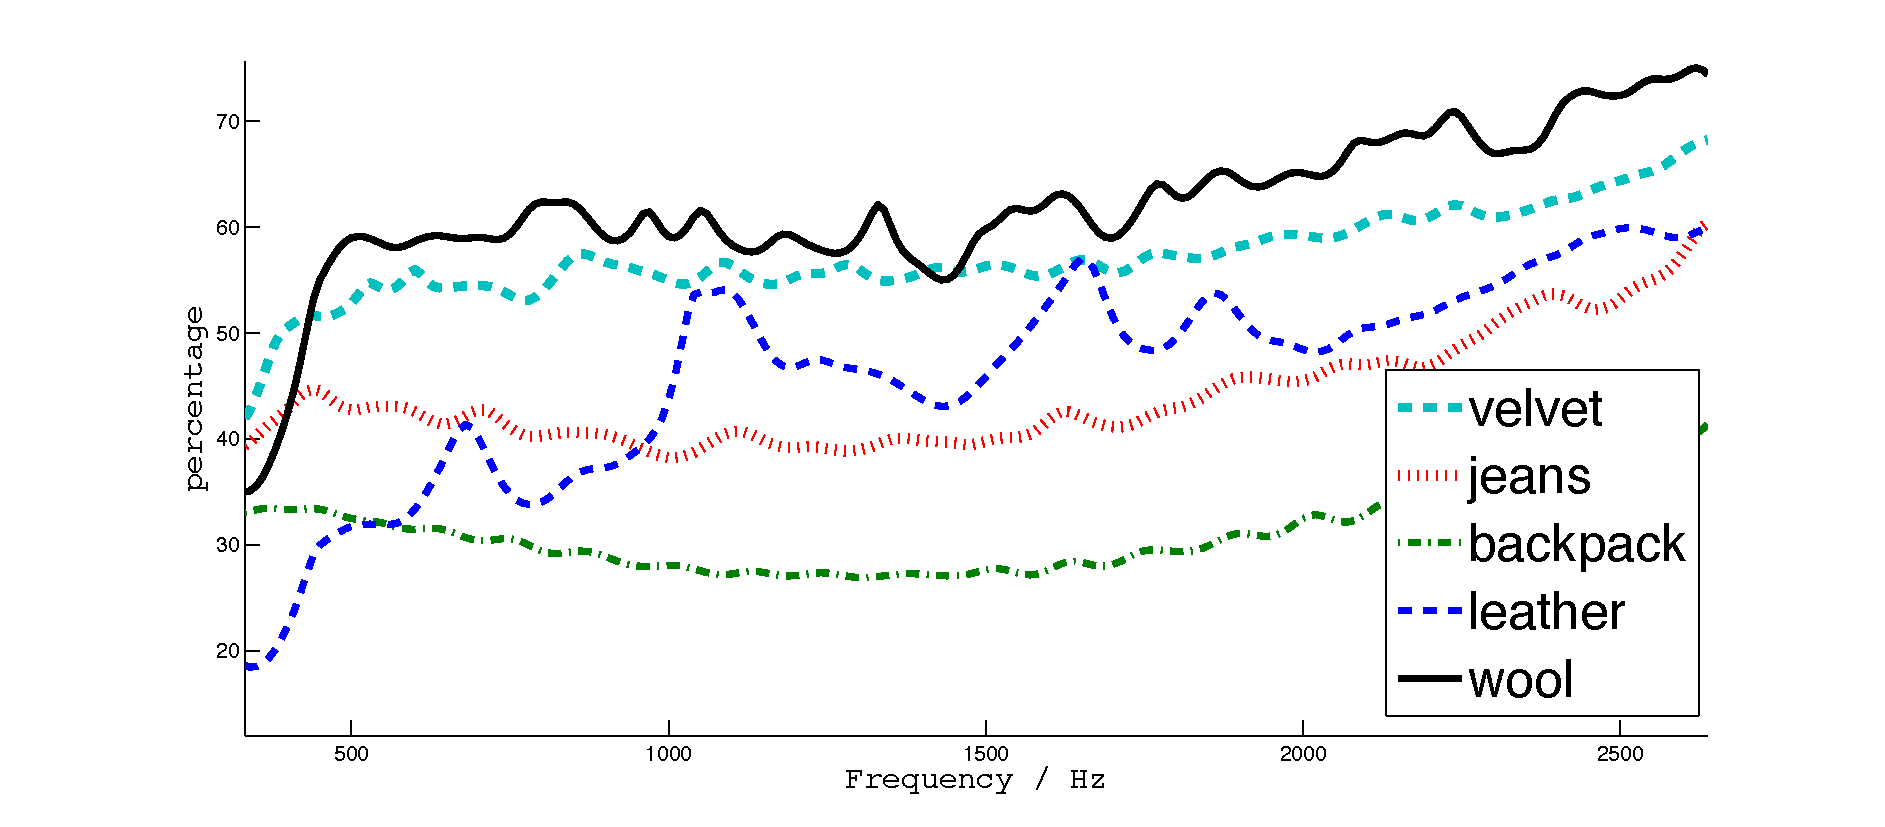
\includegraphics[height=2.5in]{soundplacement.pdf}
	\end{center}
\caption[Fabric dependent sound dampening]{Sound dampening depending on different fabric types. "White
 noise" in the frequency range from 500 to 2500 Hz is played on a
 regular pc speaker and recorded by an iphone 3gs. The iphone speaker
 is covered with the given fabric types. The plot shows the
 percentage difference between the clean recorded signal and the
 recordings obstructed by fabric. Each fabric has a distinct absorption spectrum.}
\label{fig:soundplacement}
\end{figure}

Changes in device placement affect sound to a much higher degree.
Different environments have their distinct sounds. As shown in
Figure~\ref{fig:soundplacement}, when the microphone of a device is
obstructed by specific material, frequency dampening is to be
expected. This is bad, if we try to classify sounds in the
environment. On the other hand, this dampening is distinct for the
given placement, therefore it can be used to determine the
location. This fact is explained in closer detail when we look at the
technical background of our method in section~\ref{onoff:background}.

\begin{figure}[t]
  \begin{center}
  \includegraphics[height=2.5in]{sigstrengthRoom.pdf}
	\end{center}
\caption[Wifi signal strength for different rooms]{Wifi signal strength recorded by a mobile phone in
 different rooms of the same building. The phone is put on a desk
 for 5 minutes stationary in several rooms. The experiment is
 repeated 15 times. We show the mean average signal strength in dBm
  for three rooms: office, lab and commons. The difference in strength between rooms is statistically
 significant.}
\label{fig:sigstrength1}
\end{figure}

The environmental impact on radio waves is well known and
applied. There are several commercial efforts and an extensive
research body using these impacts, for example, for indoor location
technologies~\cite{hightower2001lsu, 1067190}. Radio waves, however,
are not only influenced by the environmental placement, but also by
their immediate surroundings; radio waves in the 2 GHz range, for
example, are obstructed by large amounts of water (e.g. the human body). As seen in
Figure~\ref{fig:sigstrength1}, the signal strength from several wifi
access points is distinct in different locations. However, the signal
strength also highly depends on the on-body placement of the device
recording it. 

As these examples illustrate, environmental placement affects sensor
signals in a complex way. There are specific locations that can be
distinguished using just passive sensor data, yet this method is very
limited regarding general placement inference. Thus, the approach to
actively sample the environment (i.e. the device itself emits a given stimulus and analyses the
response of the environment) seems to be far more promising.


\section{Theoretical Background}
\label{onoff:background}
Our method is derived from the observation that a ringing mobile phone
sounds differently depending on where it is located. Whereas a phone
in a jacket pocket sounds 'dampened', a phone on a metal cabinet can
make the entire cabinet resonate. This is true for a ringing phone as
well as for a merely vibrating phone. We, thus, propose to use sound from
a built-in speaker and vibration from a built-in vibro-motor to create
a mechanical "excitation" of the environment and analyze the response
with an accelerometer and a microphone.

%a microphone. In an extensive experimental 
%study (47 locations with total of 1200 data points) 
%we demonstrate that two types of information can be derived from this analysis. 
%First, the system can be trained to recognize
%specific locations such as the 'kitchen table', or the 'dining room
%table'. Second, it can recognize more abstract locations based on
%materials such as a 'wood table', 'a closed metal cabinet', or a 
%'jacket pocket'. While this leads to less specific positioning, it has
%the advantage that the system does not need to be trained for each
%single location. Instead, after being trained on, for example, 
%several wood tables, it will recognize others it has not seen before.

%Clearly understanding how object location can be used in different
%applications is a complex topic that needs further research. 
%Nonetheless, the type of considerations sketched
%above indicates that object location is 
%a useful piece of information.
%% and finding ways to obtain it with 
%%simple, easily deployable setup a relevant research topic. 
%From this motivation we
%present and systematically evaluate a novel method for 
%object localization. The method provides so called symbolic (sometimes
%also called semantic) location (e.g. \cite{1045120})
%rather then absolute coordinates. Thus the output of the system is of
%the type 'on the couch' or 'in the drawer'. 
%The key contribution of our work is to present a
%method that requires no infrastructure, relies on simple, cheap
%sensors and still produces useful results.

In abstract terms, the above method is about analyzing the response
of the environment to a mechanical "excitation" with different frequencies. 
By vibrating the device we provide a low frequency (a few Hz) and relatively high intensity (as
compared to sound) source of excitation. By emitting fixed frequency
"beeps" we generate different, low intensity high frequency stimuli.  
The accelerometer detects the low frequency response (in our case up
to 15Hz due to a device sampling frequency limit of 30Hz),
the microphone the high frequency part. 

The response to the above stimuli falls into several categories. 
First, we receive a low frequency response. 
It is directly mechanically coupled to the vibrating object and can be detected
by the accelerometer. This response can range from a more or less
complete absorption of the vibration energy (e.g. when the object is
lying on pillow) to a resonant response where the 
surface on which the device is lying, joins in the vibration.
This fact contains information on two placement properties. For one, it can reveal if, and how
the device is fixed (in the hand, in a tight pocket, lying freely). In
addition, it reveals the hardness and elasticity of the surface on which the
device is placed. This information can be expected to reliably distinguish
between soft surfaces (e.g. a sofa) and hard ones like a
table. Distinction between several similarly hard surfaces (e.g. metal
and stone) is difficult.

Second, we get a high frequency response from the vibration, 
which is essentially sound from the device hitting the
surface. Assuming the placement of the device does lead to this kind
of response (it will not, if the device is in a soft pocket or say hanging),
it is quite location specific. The sound depends not only on the
surface material but also on the overall structure. 
Thus a small, solid cube will produce a different sound
than a large thin surface, even if both are made of the same
material. Finally, objects light and close enough to the device to
be influenced by the vibration (e.g. a key chain) might also
contribute to the sound. In general, this is a source of noise rather
then usable information. 


 Third, we get a high frequency response from the beeps which
is given by the absorption spectrum of the environment.~\footnote{Note that the absorption also influences the sound caused by the device vibration.}
Clearly this response is only useful if it comes from the immediate
vicinity of the device. This can either be the surface on which the
device is lying or, if the symbolic location is a closed compartment, the
walls of this compartment (see sections 2.4 and 2.7 for a discussion of
microphone placement issues). 

\begin{table}[ht]
\caption[Frequencies and material absorption spectrum]{Frequencies and their absorption by the selected material, given as a fraction of perfect absorption\cite{olson1967mpa}.}
\centering
\scalebox{0.95}{
\begin{tabularx}{40pt+\textwidth}{l c c c c c c }
\toprule
frequency & 128 Hz &	256 Hz &	512 Hz &	1,024 Hz &
2,048 Hz & 	4,096 Hz \\
\midrule
concrete unpainted & 0.010&	0.012&	0.016&	0.019&	0.023&0.035 \\
brick wall painted & 0.012&	0.013&	0.017&	0.020&	0.023&0.025 \\
carpet on concrete & 0.09 &	0.08 &	0.21 &	0.26 &	0.27 &0.37 \\
\bottomrule 
\end{tabularx}}
\label{table:freq} 
\end{table}
 
It is well known that the acoustic absorption spectrum is a distinct
material property. The topic has been extensively studied in the
context of musical instruments and sound isolation in
construction~\cite{olson1967mpa}. Typically, the absorption is given at discrete
frequencies as a fraction of the perfect absorption of an open window
(lack of any reflecting surface) of equal area.
As an example, we consider the coefficients in Table~\ref{table:freq}.
This clearly demonstrates that, in principle, even seemingly similar materials
can be separated with a small number of discrete frequencies. 

\section{Approach}
\label{sec:approach}
\paragraph{Procedure Description}
The proposed method consists of two parts. Each part can be used
individually or in combination with the other.

The first part is based on vibrating the device using a 
vibration-motor of the type commonly found in mobile phones. During
the vibration, which last a couple of seconds, motion data is recorded with
an accelerometer and sound with a microphone. The motion and sound
signals are used separately for an initial location
classification using standard feature extraction and pattern 
recognition methods. The final classification is obtained
through fusion of the two classification results. 

The second part is based on sound sampling. The device emits a series
of beeps, each in a different, narrow frequency spectrum. The
microphone is usually positioned is such a way that it receives only little energy
directly from the speaker. Instead a significant part of the energy
comes from reflections from the immediate environment (see bellow 
for a more detailed discussion). For location
recognition the sound received from the different beeps is compared. 

When the two parts are used together, the corresponding results are
fused using an classifier fusion method. 

\paragraph{Applying the Procedure: Specific Locations vs. Location Classes}
 Our method provides information on
abstract properties such as surface material as well as information
on properties characteristic of a single specific location (e.g. a
solid cube vs. large surface with several legs). As a consequence this
chapter investigates two different usage modes of our method:
\begin{enumerate}
\item "Specific Location Mode". In this mode, we train the system on
 concrete locations such as a specific table or a specific chair. The advantage of this approach is that the user
 is provided with exact location information. The main disadvantage is the
 effort involved in training each individual location. In addition,
 there is the question of being able to distinguish a large enough number of
 locations to satisfy relevant applications. 
\item "Abstract Location Class". In this mode, we group locations into
 abstract classes. The two main criteria are the surface material and
 being open (e.g. tabletop) or closed (e.g. inside a cupboard). In
 this mode the system is trained on several instances of each
 class. It is then able to recognize other arbitrary instances of
 this class. Thus the training problem is avoided, as the system can
 pre-trained at 'production time' and given to users without the need
 for further training. The disadvantage lies in the less exact
 location information, which has to be further interpreted and/or
 combined with additional information to find out where the object is
 actually located.
\end{enumerate} 

\subsection{Issues to Consider}
\label{sec:issues}
\paragraph{Microphone and Speaker Placement}
As described above, for the analysis of the absorption spectrum we must
ensure that the sound emitted by the loudspeaker is reflected from the
surface on which the device is lying and/or, in case of the symbolic
location being a closed compartment, from the compartment walls. The
second part is trivial. The first implies an appropriate placement of
the microphone and the speaker. 
Optimally the speaker and the
microphone should be located close to each other
on the side of the device, preferably (but not necessarily) 
facing downwards with a sound proof
barrier blocking the direct sound path between them. The main problem
in implementing this type of setup is the definition of "on the side"
and "downwards". In the worst case, we could be dealing with a cubic
or round object with no preferred "down" or "side". For such an object,
two speakers located at a 90 degree angle 
need to be used to ensure that there is always a sidewards
facing one. Our experiments (see section \ref{sec:experimental})
indicate that the position of the microphone is less critical and we
achieved good results despite the microphone facing upwards, so that
one microphone might suffice. 

%It is interesting to note, that the results of our experiments indicate
%that optimal placement is not critical. The NOKIA mobile phone
%used in the experiments indeed has a loudspeaker on the side (upper
%side see figure \ref{fig:nokia}) facing towards the back side. If
%placed in the usual position (back side down) this means that the
%loudspeaker is facing downwards towards the surface. 
%However the microphone is on the
%front side (which is then the upper side) on the lower end of the
%phone. This is a quite typical layout for modern mobile phones which
%ensures that the 'hands-free' speaker will not be accidentally put to
%the ear when on.
 
\paragraph{Variations within Symbolic Locations}
Many symbolic locations such as "table" or "desk" 
have considerable physical dimensions. This means that the response to
the mechanical stimuli may be subject to spatial
variations. For example, the low frequency 
response to vibration (acceleration data) may be different over the
leg of a table than in its middle. Similarly, on a table adjacent to the
wall, the response to the "beep" will vary depending on how close to
the wall the device has been placed.
As a consequence, for both, training and testing, a sufficient number
of random physical locations must be sampled for each symbolic
location (as has been done in experiments described in section \ref{sec:experimental}).

\paragraph{Number of Relevant Locations}
Clearly there are limits to how many locations can be reliably
recognized. In common environments
such as home or office, there are many 
places where objects can be put. The question is, whether the
number of locations that can be distinguished is sufficient to be
useful in relevant applications. An authoritative answer to this
question can only be found through an analysis of specific 
applications. Subsequently, we make no claim for such an answer,
we focus on the technology merits instead, demonstrating the
following:
\begin{enumerate} 
\item Our system shows reasonable recognition performance even using
 the combined data set of 35 locations. In our experiments these are
 collected from 3 rooms. It seems unlikely that this would not
 be sufficient covering all relevant symbolic locations in a 
 single room. At the same time, room level location of RF enabled sensor nodes is a manageable problem. 
\item Provided that an adequate number of sufficiently abstract
 classes is chosen, the issue of the number of locations is avoided by the
 "abstract location classes" usage mode. In the experiments, we
 demonstrate near perfect recognition for 7 and reasonable results
 for 12 classes. The type of classes used in the experiments ("open
 wood surface", "closed wood cabinet" etc.) is clearly abstract
 enough to describe a large number of locations. 
\end{enumerate} 

\paragraph{Sensor Requirements}
In the introduction we have stated our aim of developing a method
suitable for smart objects. Accelerometers and a microphones are
among the most widely used components in small sensor nodes. Small
loudspeakers capable of emitting beeps are also commonly integrated in those
nodes. As will be described in section \ref{sec:recognition} 
we work with frequencies between 500 and 4000 Hz, which can be handled
by small, cheap speakers and microphones. Finally, although 
vibration motors have so far not been used in sensor nodes, they are
available in sizes around 1cm and smaller (see figure \ref{fig:vibmot})
at reasonable costs. 

In summary it can be said that the proposed sensor configuration is 
compatible with the target domain of small, cheap smart objects. 

\paragraph{Complexity}
Any method that is to be deployed on low end sensor nodes and smart
objects needs to be resource conscious.
However, when considering the method proposed in this paper it is important to
remember that it is not meant for continuous tracking of a
moving device. Instead we assume that the method runs once
after the acceleration sensor has detected that the device has been
moved and is left to rest. Therefore, speed and power efficiency of the algorithm
are not so essential. We just need to
show that with typical resources available in such nodes
it is feasible to either perform the required computation or transmit
the data to a remote server for processing.
For the sake of simplicity, we restrict ourselves to the
communication requirements of the raw data.
With 16 bit resolution and the sampling rates
given in section \ref{sec:recognition} we require a data rate of about
130 Kbps for the sound and a about 5 Kbps for the acceleration. These rates
have to be sustained for a total of 13 seconds.

With respect to online execution, we merely point to related work by
our group in which we have studied implementations of sound and
acceleration based activity recognition\cite{1033880}. With sampling rates, features
and classifiers similar to the ones proposed in this paper we were able
to demonstrate power efficient execution on nodes using the TI MSP 430
microcontroller with less then 100K of RAM. 
Therefore, a sensor node should be able to execute the proposed method
--or at least computing most of the features (in particular the FFT)--
to avoid transmitting the raw sound data.

%\subsection{Usage Modes and Limitations}
%As stated in the introduction 
\section{Recognition Method}
\label{sec:recognition}
As described in section~\ref{sec:approach}, our approach can be divided into two distinct methods, mechanical vibration and sound sampling. 

\begin{table}[ht]
\caption{Features used for frame-by-frame classifications}
\begin{center}
\begin{tabularx}{\textwidth}{XX}
%{p{1.95in}p{2.95in}}
\toprule
Feature Name& Description\\
\midrule 
Standard features& Zero Crossing Rate, median, variance, 75\% percentile, inter quartile range\\
\midrule 
Frequency Range Power& computes the power of the discrete FFT components for a given frequency band. \\
\midrule 
Sums Power Wavelet Determinant Coefficient 
& describes the power of the detail signals at given levels that are derived from the discrete wavelet transformation of the windowed time-domain signal. This feature has successfully been used by \cite{sekine2000}. \\
\midrule 
Root Mean Square (RMS)&$\sqrt{\frac{1}{N}*\sum_i{x_i^2}}$, with $N$
the number of samples in a sliding window, and $x_i$ the i'th sample of the window.\\
\midrule 
Number of Peaks& The number of peaks in the window with different thresholds, low medium and high.\\
\midrule 
Median Peak Hight& The median of the peak hight. \\
\bottomrule
\end{tabularx}
 \label{table:features}
\end{center}
\end{table}

\subsection{Vibration}
During the vibration phase, the device itself records the sound and the
acceleration. Figure~\ref{fig:soundVib} and Figure~\ref{fig:accelVib} show some signal examples for
sound and acceleration recorded in different symbolic locations. Classification is performed separately on
each signal and the information of the two
modalities is combined on classifier level (see Section~\ref{sec:fusion}).


\begin{figure}[t]
  \begin{center}
  \subfloat[]{\includegraphics[trim=10 0 10 0,clip,height=1.7in]{carpetfloor-vib.pdf}
  	\label{fig:carpetVib}}
  \subfloat[]{\includegraphics[height=1.35in,height=1.7in]{desk-vib.pdf}
  	\label{fig:deskVib}}
   \end{center}
\vspace{-10pt}
\caption[Sample vibration sound spectrum]{
The vibration sound spectrum recorded for a carpet, on the left, and a desk, on the right.}
\label{fig:soundVib}
\vspace{-10pt}
\end{figure} 

\paragraph{Vibration Sound Processing}
About 30 individual features are calculated
over a 500 msec. sliding window (250 msec. overlap). We
pick 5 based on initial tests: the zero
crossing rate, the frequency range power, 75\%Percentile, sums power
wavelet determinant coefficient and the median (see Table~\ref{table:features}). We
trained common machine learning algorithms using these features, e.g. K-NN, Naive Bayes, C
4.5. As all machine learning algorithms provid comparable results and we need a ranking mechanism for the different
classes, we use the Naive Bayes classifier in the following. 
The frame-by-frame output provided by the Naive Bayes classifier is
smoothed using a majority decision over the entire length of a single
vibration phase. We also perform experiments using Hidden
Markov Models either on the features calculated in the 500ms windows
or on the classifier output of the frame by frame classifier. Since
none of the above produced significant improvement, we use
the less computationally intensive majority decision.


\begin{figure}[t]
  \begin{center}
  \subfloat[]{\includegraphics[height=1.7in]{bed.pdf}
  	\label{fig:bed}}
  \subfloat[]{\includegraphics[height=1.7in]{stereo.pdf}
  	\label{fig:stereo}}
   \end{center}
\vspace{-10pt}
\caption[Acceleration norm examples]{
The acceleration norm from 
bed~\subref{fig:bed} and the stereo~\subref{fig:stereo}. On the x-axis are the samples (30 per second) and on the y-axis the magnitude. The accelerometer on the Nokia 5500 Sport discretizes the values between +/- 600, 250 being 1 g.}
\label{fig:accelVib}
\vspace{-10pt}
\end{figure} 


\paragraph{Vibration Acceleration}
The process described above for the vibration sound is essentially
repeated for the acceleration. The only differences are the length of
the window  (1 sec with 0.5 sec. overlapping) and the final feature
set (variance, the RMS, number of peaks, median peak height, the
75\%Percentile, inter quartile range). 

\subsection{Sound Sampling}

\begin{figure}[t]
\centering  
\includegraphics[scale=0.36]{beeps.pdf}
\caption[Audio fingerprint sample]{The played fingerprint audio, with the distinct frequencies, on the left in the time domain, on 
the right in the frequency domain.}
\label{fig:beeps}
\end{figure}

\begin{figure}[t]
  \begin{center}
  \subfloat[]{\includegraphics[height=1.7in]{drawer.pdf}
  	\label{fig:drawer}}
  \subfloat[]{\includegraphics[height=1.7in]{backpack.pdf}
  	\label{fig:back}}
   \end{center}
\vspace{-10pt}
\caption[Time domain audio fingerprint examples]{
The audio fingerprints for drawer and backpack in the time domain}
\label{fig:soundfing}
\vspace{-10pt}
\end{figure} 


\begin{figure}[t]
  \begin{center}
  \subfloat[]{\includegraphics[height=1.7in]{shelffingerprint.pdf}
  	\label{fig:backf}}
  \subfloat[]{\includegraphics[height=1.7in]{backpackfingerprint.pdf}
  	\label{fig:drawerf}}
     \end{center}
\vspace{-10pt}
\caption[Frequency domain audio fingerprint examples]{
The audio fingerprints for drawer and backpack in the frequency domain}
\label{fig:soundfingt}
\vspace{-10pt}
\end{figure} 

The active sound sampling procedure differs from 
the vibration method in several 
ways. We know from literature (see section \ref{sec:approach}) that
few discrete frequencies between a few hundred and a few thousand Hz are enough to separate a large range of
materials in terms of their absorption coefficients. Therefore, we 
select 8 discrete, equidistant frequencies 
between 500 and 4000. Figure~\ref{fig:beeps} shows the signal emitted by the speaker in time and frequency domains. 
The frequency range choice is dictated
by the specification of small, cheap speakers (not capable of very low
frequency tones) and available sampling rates -the used mobile phone is just capable of sampling
with 8000 Hz. Some sample recordings for different symbolic placements can be seen in
Figure~\ref{fig:soundfing} (in the time domain) and in Figure~\ref{fig:soundfingt} (in the frequency domain). 
From the recorded beeps we first isolate 8 frequency fingerprints
using a variable intensity threshold. As features we empirically select
RMS, frequency range power and the sums power wavelet determinant
coefficient using the mutual information metric. These features 
are determined out of 30 features calculated using a 200
msec. sliding window with 150 msec. overlap.

The features of all 8 frequency prints are combined into one feature set.
This means that a feature instance contains the calculated RMS etc. of each 
frequency band. The rest of the procedure is identical with the 
vibration recognition (frame by frame classification using C 4.5 and
majority decision). 

%Machine learning algorithms are trained on the feature set, here again we picke
%d the C.4.5 as final classifier. On top of the frame-by-frame classification a 
%majority
%voting is employed for the complete duration of the recorded sound sample.

\subsection{Fusion}
\label{sec:fusion}

\begin{figure}[t]
\centering  
\includegraphics[scale=0.66]{recognition2.pdf}
\caption{The fusion recognition method as overview.}
\label{fig:recognition}
\end{figure}
The two main approaches to fusion are signal/feature level and
classifier level fusion. Feature level fusion works best for features
that are computed at the same sampling rate (sliding window size).
This is not the case for the three recognition modalities described
above. As the different window sizes are determined heuristically to
produce best results for each modality, dropping them for the sake of
fusion makes little sense. As a consequence, no direct feature level
fusion is investigated. We, however, investigate a fusion
approach based on the results of the 
frame by frame classification (see Figure~\ref{fig:recognition}). This can be viewed as a kind 
of feature level fusion, since its result is
input to the majority decision. Thus, we compute
the majority decision for an event over the frame by frame results
from all three modalities put together, instead of computing it for
each modality separately.

In terms of classifier fusion we opt for a Bayesian Belief
Integration method (see \cite{ruta-overview} for an overview of
classifier fusion methods). This method uses the confusion matrix
obtained from testing the classifiers on the training data set to
determine class probabilities for different combinations of
classifier outputs. This allows the system to take into
account the peculiarities of each classifier. 
With just 3 classifiers and a constrained number of classes 
it is also computationally tractable. If the number of classes 
is increased the method could be replaced by e.g. logistic regression.

\begin{figure}[t]
  \begin{center}
  \subfloat[]{\includegraphics[trim=10 0 10 0,clip,height=1.7in]{appartment.pdf}
  	}
  \subfloat[]{\includegraphics[height=1.35in,height=1.7in]{livingroom.pdf}
  	}
 \subfloat[]{\includegraphics[height=1.35in,height=1.7in]{office.pdf}
  	}
	\\
\subfloat[]{\includegraphics[height=1.35in,height=1.7in]{room.jpg}
  	\label{fig:room}}
\subfloat[]{\includegraphics[height=1.35in,height=1.7in]{home.jpg}
  	\label{fig:home}}
\subfloat[]{\includegraphics[height=1.35in,height=1.7in]{office.jpg}
  	\label{fig:office}}
   \end{center}
\vspace{-10pt}
\caption[Experiment environment]{The top figures show schematics of the rooms used for the experiments. 
The symbolic locations we try to detect are marked in red for the apartment living room and office. 
Below the schematics there are actual photos from the locations.}
\label{fig:experiment}
\end{figure} 


\section{Experimental Validation}
\label{sec:experimental}
During the evaluation, we design and conduct experiments for both modes of our method,
specific and abstract location. We always introduce the details to the specific location mode first,
going into details about the scenario and procedure.

%An important concern in the design of the experiments was to work with
%realisti scenarios and not only demonstrate where our method works,
%but also show where are the limits.

\subsection{Validation Scenarios}
\subsubsection{Specific Location Mode}
As basis for our study, we pick three scenarios: 
an office, a living room, and a
one room student apartment. In each scenario a set of obvious locations
for placing objects are selected. These include the
furniture present in the room (both open such as table or sofa and
closed such as cupboards), the floor, the window ledges and additional
objects such as the stereo. In the
office scenario we also include three pockets (two different
pockets of a jacket and a jeans pocket), the inside of a backpack
and a suitcase as well as a trashcan. 
A full listing of the investigated location is given in
Table~\ref{table:location} and illustrated in
Figure~\ref{fig:experiment}. There are 16 locations in the
office, 9 in the living room and 10 in the apartment (total of 35).


We record 30 experimental runs on each specific location (a total of
over 1000 events), each time randomly varying the exact position of the recording. 
The object is placed according to positions drawn randomly from a uniform distribution.
Of the 30 runs, 10 are randomly picked to train the classifiers, the remaining 20 are
used as test set. Evaluation is performed
first on each individual scenario (assuming that room level
location could be obtained by other means). We also perform an evaluation on a data set containing all
locations from the three scenarios, to see how our method
behaves when the number of locations increases.

\begin{table}[ht]
 \caption[Symbolic locations picked for the experiments]{Chosen symbolic locations and abstract location classes. 
The letter in front is the identification
 for the individual confusion matrix plots presented later in the paper. The letter in brackets behind the class description, is the
 identifier for the confusion matrix plot over all 35 locations. In j. , o. j. and tr. pocket stand for inside jacket, outside jacket and trousers pocket. }
\scalebox{0.82}{
\begin{tabularx}{75pt+\textwidth}{lllll}
\toprule
Office& &Living room&Apartment&Surfaces\\
\midrule
a. backpack(a)&k. in j. pocket(C) & a. desk(h)& a. bath carpet(f)& a. polster open\\
b. cupboard(z)&l. tr. pocket (e)& b. floor(u)  & b. bed(p)&b. glass open\\
c. suitcase(w)&m. cartbox (F) & c. sofa(n)& c. chair(b)& c. iron open\\
d. drawer(t)& n. ledge (H) &d. table(A)& d. desk (wood) (l)& d. stone closed\\
e. desk(D)& o. chair (v) & e. chair(c)&e. radiator(d)& e. wood closed\\
f. top drawer(E)&f. drawer (m)& f. ledge(k)& f. glass closed\\
g. cabinet (x)& p. shelf (i) &g. ledge (G)& g. carpet floor(B)& g. iron closed\\
h. o j. pocket(j) & & h. stereo (s)& h. cupboard(g)& h. metal open\\
i. trashcan(I)& & i. tv (j)& i. drawer(q)& i. polster closed\\
j. carpetfloor(r)& & & j. wardrobe (o)& j. stone open\\
\bottomrule 
\end{tabularx}}
\label{table:location}
\end{table}

\subsubsection{Abstract Location Type Mode}
The abstract location types are defined according to the surface
material and the location being open (e.g. a table) or closed (e.g a
cabinet or a drawer). As shown in Table \ref{table:location} this
lead us to 9 classes including most typical surfaces (wood, glass
metal, stone, cushion). To get a sufficient number of different instances
for each class we record the data in a furniture store. For
every abstract class we pick 6 different pieces of furniture. Two
recordings are conducted on each specific piece of furniture leading to 9
data points per abstract class and a total of 144 events. For the
evaluation two pieces from each class (four events per
class) are picked for training and 4 (8 events per class) are
retained for testing. This is consistent with the envisioned
application use case in which the user would be given a device "factory 
pre-trained" for each class and use it to recognize instances of the
class not seen by the system before. 

\subsection{Experimental Procedure}

\subsubsection{Setup}


\begin{figure}[t]
\centering  
 \subfloat[]{\includegraphics[trim=10 0 10 0,clip,height=1.9in]{vibmot.jpg}
  	\label{fig:vibmot}}
  \subfloat[]{\includegraphics[height=1.35in,height=1.9in]{speaker.jpg}
  	\label{fig:speaker}}
\caption[Vibration motor and phone loudspeaker]{A picture of a common vibration motor and the extra loudspeaker on the Nokia 5500 Sport.}
\label{fig:hardware}
\end{figure}
For the experiments, we use the Nokia 5500 Sport, see Figure~\ref{fig:hardware}. It is a mobile phone of Nokia's third S60 series, equipped with an accelerometer and an extra loudspeaker. The mobile is able to run C++, Java and python code. We record data using python.
The evaluation is done in batch processing using a mixture of Python, Matlab scripts and Java code, mainly consisting of the Weka machine learning package.

\begin{figure}[t]
  \begin{center}
  \subfloat[]{\includegraphics[trim=10 0 10 0,clip,height=2in]{appartmenttraining.pdf}
  	\label{fig:apptraining}}
\subfloat[]{\includegraphics[trim=10 0 10 0,clip,height=2in]{livingroomtraining.pdf}
  	\label{fig:livingtraining}}
	
	
  \subfloat[]{\includegraphics[height=1.35in,height=2in]{officetraining.pdf}
  	\label{fig:officetraining}}
   \end{center}
\caption[Accuracy versus training samples]{ The classification accuracy depending on the number of training events and different sensing modalities for the appartment \subref{fig:apptraining}, 
living room \subref{fig:livingtraining}, and office scenario \subref{fig:officetraining}.}
\label{fig:training}
\end{figure} 


\subsubsection{Data Acquisition}
An experimental run consists of the following steps. First the phone
is placed on a random spot on a particular location. Using a uniform
distribution, the actual spot is determined randomly. Then the
measurement is started. While the mobile vibrates for 5 sec. lying
face up on the surface, the sound from the phone
vibrating is sampled by the on-board microphone with 8
kHz and the acceleration with 30 Hz. After the vibration measurement
is done the mobile plays the sound sample consisting of 8 beeps in
distinct frequencies from 500 to 4000 Hz in 500 Hz steps (as seen in Figure~\ref{fig:soundfing}). Each tune is
1 sec. long. While the mobile plays this using the extra loudspeaker,
the python script records the sound with 8000 Hz over the built-in
mobile microphone. The loudspeaker faces the surface, as depicted in
Figure~\ref{fig:hardware}. We get around a problem of accessing
full-duplex mode in python on the Nokia phone by using the music
player and the extra speaker.


\begin{figure}[t]
  \begin{center}
  \subfloat[]{\includegraphics[trim=10 0 10 0,clip,height=1.8in]{barchart1st.pdf}
  	\label{fig:barchart1}}
  \subfloat[]{\includegraphics[height=1.35in,height=1.8in]{barchart2nd.pdf}
  	\label{fig:barchart2}}
   \end{center}
\caption[Classification performance per scenario]{ Barcharts for living room, office, apartment, and abstract
 classes using just the first result of the
 classification~\subref{fig:barchart1} and allowing the 2nd best
 vote~\subref{fig:barchart2}}

\label{fig:barcharts}
\end{figure} 



\begin{figure}[t]
\centering  
\includegraphics[scale=0.36]{barchartall.pdf}
\caption[Classification performance over all]{Barchart for office living room, apartment and all combined
 including 1st 2nd 3rd best} \label{fig:barchart3} \end{figure} 



\subsection{Experimental Results} \label{sec:results}

The recognition performance for different scenarios, experiments and 
recognition modalities are summarized in
Figure \ref{fig:barchart1} for the three individual scenarios of
the specific location mode and the abstract location class and
in Figure \ref{fig:barchart2}, combining all 3 locations and second/third best voting.
Additionally, examples of confusion matrices are visualized for the
office scenario, the combination of all three specific location mode
scenarios and the abstract location type mode in Figures
\ref{fig:conf1}, \ref{fig:all} and \ref{fig:confmasurf} respectively.
The dependency of the classification accuracy on the number of training events can be seen 
in Figure~\ref{fig:training} for the different scenarios.

In the more detailed discussion of the results given below and the
some of the figures we at times discuss "2nd best evaluation" or "3rd
best evaluation". This refers to cases where the correct class
is among the 2 or 3 first picks of the classification system. 



\paragraph{Office}
In the office scenario, 14 of the 16 locations can be classified with
near perfect accuracy. The single biggest confusion is between the
pocket on the inside of the jacket and the one on the outside. This
is plausible and to be expected. An unexpected result is the poor
recognition of the metal window ledge. It is confused with the
cart-box, the top shelf and the chair. 

The classification accuracy is 54\% using the event-based acceleration
classifier, 77\% for vibration sound, 91\% for the sound sampling,
77\% and 79\% for the vibration fusion cases. We reach up to 93-94\%
for the majority decision and lookup-table fusion using all
modalities. The sound sampling is the best non-fusion method with
91\%. The "2nd best evaluation" pushes the correct classified up to
96\%.

\begin{figure}[t]
  \begin{center}
  \subfloat[]{\includegraphics[trim=10 0 10 0,clip,height=1.9in]{93perOffice.pdf}
  	\label{fig:conf1}}
  \subfloat[]{\includegraphics[height=1.35in,height=1.9in]{96perOffice.pdf}
  	\label{fig:office2nd}}
	\\
  \subfloat[]{\includegraphics[trim=10 0 10 0,clip,height=1.9in]{80perAll.pdf}
  	\label{fig:all}}
  \subfloat[]{\includegraphics[height=1.35in,height=1.9in]{94perAll.pdf}
  	\label{fig:all3rd}}
  \end{center}
\caption[Confusion matrices for the distinct classes]{ The confusion matrix~\subref{fig:conf1} of the office
 using the lookup-table fusion compared with the confusion matrix
 in~\subref{fig:office2nd} using the second best locations in
 addition to the lookup-table. The same is depicted, below only for
 all the 35 different semantic locations. Figure~\subref{fig:all}
 shows the classification of the lookup-table fusion, whereas
 Figure~\subref{fig:all3rd} shows the lookup-table fusion considering
 up to the 3rd best.}
\label{fig:confma}

\end{figure}

\paragraph{Living room}
In the living room scenario, most of the samples from 7 of the 9
locations can be classified correctly. A lot of the sofa instances are
confused with the chair, as the chair is also padded. This is the
worst confusion occurring. Again the classifiers perform poorly for
window ledge category. The living room classification accuracy starts
with 60\% for acceleration alone, and goes up to 87\% for the
vibration sound. In this scenario, the sound sampling is worse than
the vibration methods at 85\%. This explains also why the fusion
methods on top of the vibration work so well and are nearly as good as
the fusion over all methods, at 88 and 89\% respectively. The fusion
over all methods is just 0.5\% better, namely 89.5\%. Only a very
small number of events (one to two) are corrected by this fusion. In
the "2nd best evaluation" the accuracy ranges from 66\% for
acceleration alone, up to 97\% for the lookup-table fusion over all
methods. Here also, the acceleration and sound vibration fusion do
extremely well with 93\% and 96\%.

\paragraph{Apartment}
In the apartment case, the worst miss-classification happens in the
cupboard class, which is confused with the desk. Both are made out
of the same wood. The radiator class is also confused with several
other classes. Here the acceleration accuracy is at 65\%, the
vibration sound at 81\%, sound sampling at 90\%. The fusion using just
the vibration method is at 82\% and 84\% respectively. As with all the
fusion examples the lookup-table performs slightly better. Finally, the
fusion techniques on all 3 modalities are all over 90\%. Taking a
look at the "2nd best evaluation", there the accuracy ranges from 80
\% for acceleration to up to 99\% for the look-up table over all three
classifiers.

\paragraph{Combined over all rooms (35 classes)}
As expected, more classes signify a worse classification rate. The ledge classes perform
poorly, even in the 2nd and 3rd best evaluation. Also, one of the
table classes does badly and is confused with several other classes.
The classification accuracy over all 35 semantic locations is
expectably lower than those of the single scenarios, ranging from 26\%
for acceleration, 51\% for vibration sound, 74\% for sound sampling,
over 52\% for the vibration fusion, up to 78\% for the fusion of all
methods. The 2nd and 3rd best evaluations look considerably
better. Second best is up to 90\%. Third best reaches 94\%. 

\paragraph{Abstract Location Classes}
For the abstract classes, the iron and wood classes are easily
confused, as are the stone and glass. Acceleration classification
alone performs reasonably well, at 63\% compared to the other
scenarios. Sound vibration is better at 69\%. As nearly always, sound
sampling performs better than the vibration method, at 81\% accuracy.
Regarding the fusion techniques, there is also nothing surprising. The
vibration fusion majority decision is at 70\%, the vibration
lookup-table around 71\% accuracy. The two fusions based on all
methods are at 83\% for the simple majority decision case and 86\% for
the lookup-table. Allowing the second best classification method, one
can stem up the performance to 92\% for the lookup-table fusion
method.

\begin{figure}[t]
  \begin{center}
  \subfloat[]{\includegraphics[trim=10 0 10 0,clip,height=2.0in]{surf.pdf}
  	\label{fig:surf}}
  \subfloat[]{\includegraphics[height=1.35in,height=2.0in]{surf2nd.pdf}
  	\label{fig:surf2nd}}
  \end{center}
\caption[Confusion matrices for the abstract classes]{ Confusion matrix~\subref{fig:surf} of the abstract classes
 compared with the corresponding 2nd best confusion matrix
 in~\subref{fig:surf2nd}} \label{fig:confmasurf} \end{figure}



\subsection{Lessons Learned and Implications} 


\paragraph{Overall Performance}
The performance of the system is extremely inhomogeneous with respect
to the classes. There is a large proportion of classes for which the
classification is perfect or near perfect, and a small one with very
poor performance (see confusion matrices in figures \ref{fig:conf1},
\ref{fig:office2nd}, \ref{fig:all} and \ref{fig:all3rd}. As a
consequence the overall recognition accuracy figures are strongly
influenced by a few classes. This
is best exemplified by the abstract location type confusion matrix and
3rd best evaluation of the combined specific location classes. As can
be seen in the plots \ref{fig:conf1}, \ref{fig:office2nd},
\ref{fig:all} and \ref{fig:all3rd} the former has 8 perfect or near
perfect classes, 1 reasonably good class and 3 very poor ones. The
latter has 31 perfect to very good (27 perfect) classes, 1 mediocre
one and 3 very poor classes.
 

\paragraph{Class by Class Performance}
For some of the classes such as the inside and outside pocket, poor
performance is expected, as they are included to test the limits of
the system. In fact the recognition for these locations is better than
expected. Better than expected recognition has also been achieved in a
number of locations that were included as 'hard cases' such as the
backpack and the trousers pocket. Surprising is the poor performance
of the window ledge and the radiator. At this stage we have no
verified explanation. One possibility is a spatial inhomogeneity of
those symbolic locations. On the ledge, sound sampling is certainly
different depending on whether the speaker faces the window or faces
away from it. 
 
\paragraph{Value of the 2nd and 3rd Best Evaluation}
The performance of the system is particularly appealing for
applications that can accept a choice of two or three most probable
locations as system output. This has already been mentioned for the
case of 3rd best evaluation of the 35 combined symbolic locations. For
the other data sets even allowing just the 2nd best pick produces
close to perfect recognition for the vast majority of classes.

\paragraph{Value of Different Classification Modalities}
While it is to be expected from the discussion in \ref{sec:approach}
that sound sampling produces the best results and acceleration
the poorest, the difference between the two is larger than we
expected. In particular, the fact that in most cases little is gained
by adding acceleration and vibration sound to the sound fingerprint is
surprising. On the other hand, combining vibration sound and
acceleration often produces significant gains.


\paragraph{Significance of Training Set Size}
For the specific location mode the user needs to train the system for
every single relevant location. Thus the training effort is a
significant issue. As shown on the example of the office scenario in
figure \ref{fig:speaker} the system starts to display significant
recognition performance at around 5 training examples and stagnates at
about 10. We have found this behavior to be typical for all the
specific location mode scenarios. 


%
%\subsection{Paper Contributions and Organization}
%From the above discussion it can be seen that
%symbolic localization of objects with no external infrastructure
%and simple sensors suitable for small, cheap nodes is an open
%problem. This paper proposes a solution for this problem. 
%In terms of hardware the solution requires only a microphone, an
%accelerometer, a small speaker capable of emitting 'beeps' and a
%miniature vibration motor. 
%An important feature of our method is the fact that it can be used on
%both specific locations (e.g. my 'kitchen table'), and abstract location
% types. 
%
%We discuss the physical principle, key issues,
% and limitations
% behind our approach (section \ref{sec:approach}). 
%We then provide a detailed description of the recognition algorithm,
% including, feature computation,classification, and classifier fusion
% (section \ref{sec:recognition}). Finally, 
%we validate our method on an extensive, realistic data set (section
%\ref{sec:experimental}). The data set contains a total of over
%1200 measurements from 35 specific locations (taken from 3 different rooms)
%and 12 abstract location classes. The location were chosen to include
%examples that demonstrate the limits of the method such as an attempt
%to distinguish between the inner and the out pocket of the same jacket
%and between table and a book shelve both made of identical material.
%The data points at each symbolic location area taken at a number of randomized
%spots to ensure representativity.
%
%Despite such challenging evaluation our method produces promising
%results. On room bases (16, 9 and 10 locations) we
%arrive at an accuracy of between 89 \% and 93 \% with the correct answer
%being in the to 2 first picks of the classifier between 97 \% and 99 \% of the
%time. 
%With all 35 locations from the 3 rooms in one data set 
%the recognition goes down to 81 \%. However we still get the correct
%answer in the top 2 picks of the classifier 91 \% and in the top 3 94 \% times. 
%
%
%\section{Approach Overview}
%\label{sec:approach}
%\subsection{The Method}
%
%\paragraph{General Principles Behind the Recognition}
%In abstract terms the above method is about analyzing the response
%of the environment to a mechanical 'excitation' with different frequencies. 
%By vibrating the device we
%provide a low frequency (a few Hz) relatively high intensity (as
%compared to sound) source of excitation. By emitting fixed frequency
%'beeps' we generate different, low intensity high frequency stimuli.  
%The accelerometer detects the low frequency response (in our case up
%to 15Hz due to sampling frequency of the used device limited at 30Hz),
%the microphone the high frequency part. 
%
%The response to the above stimuli falls into several categories. 
%First we get a low frequency response that
%directly mechanically couples to the vibrating object and is detected
%by the accelerometer. This response can range from a more or less
%complete absorption of the vibration energy (e.g. when the object is
%lying on pillow) to a resonant response where the 
%surface, on which or device is lying, joins in the vibration.
%This fact contains information on two things. For one, it can reveal if, and how
%the device is fixed (in the hand, in a tight pocket, lying freely). In
%addition it reveals how hard and elastic is the surface on which the
%device is placed. This information can be expected to reliably distinguish
%between soft surfaces such as a sofa and hard ones like a
%table. Distinction between several similarly hard surfaces (e.g. metal
%and stone) is difficult.
%
%Second, we get a high frequency response to the vibration, 
%which is essentially a sound from the device hitting the
%surface. Assuming that placement of the device does lead to this kind
%of response (it will not, if the device is in a soft pocket or say hanging),
%it is quite location specific. The sound depends not only on the
%surface material but also on the overall structure. 
%Thus a small, solid cube will produce a different sound
%then a large thin surface, even if both are made of the same
%material. Finally, objects light and close enough to the device to
%be influenced by the vibration (e.g. a key chain) might also
%contribute to the sound. In general, this is a source of noise rather
%then usable information. Figures~\ref{fig:soundVib} show two different vibration spectra.
%
%
% Third, we get a high frequency response from the beeps which
%is given by the absorption spectrum of the environment. 
%\footnote{Note that the absorption also influences
%the sound caused by the device vibration.}
%Clearly this response is only useful if it comes from the immediate
%vicinity of the device. This can either be the surfaces on which the
%device is lying or, if the semantic location is a closed compartment, the
%walls of this compartment (see next section for a discussion of
%microphone placement issues). 
%It is well known that the acoustic absorption spectrum is a distinct
%material property. The topic has been extensively studied in the
%context of musical instruments and sound isolation in
%construction (\cite{olson1967mpa}). Typically the absorption is given at discrete
%frequencies as a fraction of the perfect absorption at an open window
%(lack of any reflecting surface) of equal area.
%As an example we consider the following coefficients from \cite{olson1967mpa}
%\\
%\noindent
%\begin{tabular}{|l|c|c|c|c|c|c|}
%\hline
%frequency & 128 Hz &	256 Hz &	512 Hz &	1,024 Hz &
%2,048 Hz & 	4,096 Hz \\
%\hline 
%concrete unpainted & 0.010&	0.012&	0.016&	0.019&	0.023&	0.035 \\
%brick wall painted & 0.012&	0.013&	0.017&	0.020&	0.023&	0.025 \\
%carpet on concrete (0.4inch) & 0.09 &	0.08 &	0.21 &	0.26 &	0.27 &
%0.37 \\
%\hline 
%\end{tabular}
% 
%The above clearly demonstrates that, in principle, even seemingly similar materials
%can be separated with a small number of discrete frequencies. 
%

\section{Excursion: Sensor Dependencies}

The successful application of our method is
highly dependent on the microphone/ speaker placement and the type of
vibration motor. A quick experimental setup illustrates this
dependence.


\begin{figure}[t]
\centering  
\includegraphics[scale=0.15]{mobiles.jpg}
\caption[Smartphones]{The three different mobile phones used for sensor
 comparisons: the iphone 3gs, nokia n95 and the htc
 desire.} \label{fig:mobiles}

\end{figure}

We use 3 regular smartphones, depicted in Figure~\ref{fig:mobiles} and
pick 4 locations from the living room scenario: desk, floor, sofa and
stereo. Each mobile performs the experimental procedure outlined in
the section above 5 times.


\begin{table}[ht]
\caption[Smartphone classification comparison]{Classification comparison for 4 locations from the living
 room scenario using frame-by-frame classification.}
\label{table:depend}
\begin{tabularx}{\textwidth+10pt }{lcccccc}
\toprule
mobile & htc desire &n95 &iphone 3gs& N 5500 Sport\\
\midrule
fingerprint & 45 \% & 60 \% & 47 \% & 100 \%\\
fingerprint (upside down) & 92 \% & 87 \% & 90 \% & 100 \% \\
vibration & 45 \% & 79 \% & 23 \% & 84 \% \\
vibration (upside down) & 43 \% & 83 \% & 25 \% & 87 \% \\
\bottomrule
\end{tabularx}
\end{table}

The classification results in Table~\ref{table:depend} show a high
dependency between the speaker /microphone placement and the
accuracy. Each phone shows respectable results with microphone and
speaker placed towards the surface using the sound fingerprint.
However, if the phones are placed with the microphone on the top (as a
phone is regularly put on a desk), the rates vary strongly, with the
N5500 being by far the best, as it has a separate speaker still facing
the surface.

Another important lesson to learn: the vibration classification seems
not that affected from the rotation of the devices. Yet, the vibration
motor and intensity seem crucial here. The HTC and iphone are
equipped with motors operating at a far lower intensity compared to
the ones built into the Nokia models. This is also the reason for the
lower classification performance.


\section{Discussion}
 
Summarizing the issues from section~\ref{sec:issues} and the
experimental results from section~\ref{sec:results} we conclude the
following:

\begin{enumerate}
\item The proposed method is well suited for low end, simple sensor
 nodes and smart objects and requires no additional positioning infrastructure. 
\item The key source of information is sound sampling. Thus if
size is critical the vibration motor can be dropped.
\item The system can reliably (90\% and more accuracy) resolve a 
sufficient number of specific locations to cover one room or a small flat. It is advisable to combine our system with room level positioning.
\item The performance of the system is extremely inhomogeneous with respect to
the classes, with most classes being recognized with high accuracy and a
few "rogue" classes showing very poor performance.
\item Settling for the two or three best picks instead of a crisp single
 classification greatly increases the number of locations that are
 reliably recognized and the tolerance towards the "rogue" classes. 
\item If training by the user is an issue, the abstract location class
 mode offers a possibility to provide "pre-trained" systems at the
 cost of more "fuzzy" location information. \end{enumerate}

Key points to investigate in the future are improved vibration
sampling (using different amplitudes and frequencies to improve
acceleration based performance), an investigation of the sources of
errors on the problematic classes, more elaborate fusion methods, and
a combination with radio signal strength based location methods. 

Summarizing, this chapter treats detecting wether a device is carried on
the body or placed in the environment as a special case of recognizing
its symbolic placement. The active sampling method presented gives a
specific solution to this recognition problem with merits and
limitations discussed above. Moving away from the detecting
environmental placements the focus is now on on-body sensing for the
remainder of this thesis, centering on how to perform activity
recognition independent of device placement and orientation,
compensating for displacements. Thus after dealing with symbolic
object placement containing locations on and off body, we focus on
determine the on-body placement of a device.


%\cleardoublepage
%\addcontentsline{toc}{section}{Bibliography}
\bibliographystyle{abbrv}
\bibliography{onoff}

 
\chapter{On-Body Placement}
\label{chapter:onbody}
    %\vspace*{\beforechapskip}%
    %\smash{\rule{2.6pt}{25mm}}
 %\chapterprecis{
\begin{flushright} 
\textit{"All models are wrong, but some are useful."
-George E. P. Box}
\end{flushright} 
%}
\begingroup %\vspace*{\beforechapskip}% %\smash{\rule{2.6pt}{25mm}}
\textit{Coarse variations related to the on-body placement of a device
  have a high impact on the reliability and effectiveness of context
  recognition systems. This chapter explores how changes in on-body
  placement impact sensing modalities commonly used in pervasive
  computing. We discuss general considerations and give some advice on
  how to make activity sensing more robust to placement changes.  We
  then present several methods to derive the coarse device
  placement solely based on rotation and acceleration signals. 
  The methods work regardless of device orientation.  We
  present an elaborate evaluation of these methods on already
  published, large scale data sets with diverse activities from
  bicycle repair to house work.  We reach a recognition rate of 80\%
  over 4 min. of unconstrained motion data for the worst scenario and
  up to 90\% over a 2 min. interval for the best scenario.}\\\\ 
K.~Kunze and P.~Lukowicz.  \newblock Using acceleration signatures
from everyday activities for on-body device location.  \newblock {\em
  11th IEEE International Symposium on Wearable Computers}, Sep 2007.
\\K.~Kunze, P.~Lukowicz, H.~Junker, and G.~Troester.  \newblock Where
am i: Recognizing on-body positions of wearable sensors.  \newblock
{\em LOCA'04: International Workshop on Location and Context Awareness
}, Jan 2005.

\vskip\onelineskip
\begin{adjustwidth}{}{-\chapindent}%
\hrulefill   
\end{adjustwidth}\endgroup
\vskip\onelineskip
\vskip\onelineskip 
After discussing general environmental placement issues, we focus on
lifting another constraint for the users: Having to place sensing devices on
well-defined positions on the body. 
\begin{figure}[t]
    \begin{center}
    \includegraphics[height=2in]{OnbodyOverview}
	\end{center}
\caption[Focus of the On-body Placement Chapter]{Thesis overview with the central question for this chapter
  highlighted.} \label{fig:onbodyoverview} \end{figure} 
Specifically, this chapter deals with coarse variations related to the body part, on 
which the device is carried (see in Figure~\ref{fig:onbodyoverview}).

A well-established approach to context and activity
recognition is the use of motion sensors (predominantly
accelerometers) attached to different parts of the user's body.
Various types of activities ranging from simple modes of locomotion
analysis to complex assembly tasks have been successfully recognized
using such sensors~\cite{seon2001recognition,bao2004activity,lukowicz2004recognizing} .  
Most research in this area, however, relies on sensors being placed at specific
locations on the body. Typically, these include the wrists, the arms,
legs, hips, the chest and even the head. Once a subset of placements
is chosen, the system is trained on this specific subset and
will not function properly if the sensors are placed at different
locations.  This implies that the user either has to explicitly "put
on" the sensors each time he dresses up or the sensors have to be
permanently integrated into the individual pieces of clothing or
devices he usually carries, e.g. a mobile phone. If devices are used,
the user is required to carry them always at the same body location, e.g. the key chain needs to be
always placed in the right trouser pocket. 

We consider this to be a very critical issue. Experience shows that
people usually have several accessories with them and vary their
on-body placement depending on the circumstance~\cite{Ichikawa:2005p6295}. In a
typical scenario the user might carry a key-chain in his trousers
pocket giving us the leg information, a watch on the wrist, a mobile
phone in a holster on the hip and a smart card in the wallet in a jacket
pocket. A flexible context recognition system could then 
determine the on-body location of the devices to use them for an inference task.

Location information in itself is an interesting part of
context. As an example, knowing if glasses are worn or if they are in
a pocket can be an important clue to the user's activity.

The work described in this chapter is a major step in our effort to
facilitate the adaption of context recognition
with one focus: learning the device placement on the body. We
illustrate on-body placement issues on sensor modalities common in
activity sensing. Then, we explore how to classify different body
placements. To assess the feasibility, we start with a very
narrowly defined activity, namely "walking". We demonstrate how to
detect "walking" in a device placement independent way and then
leverage this to detect the device placement. In the following, we can abstract a
more general model, no longer constraint to 'walking'. The model works for a broad range of common human
activities tested in a large scale experimental evaluation.

% We then demonstrate how the
%information that the user is walking can be leveraged to determine
%device location.



\section{Impacts of the Body Part Placement}
\begin{figure}[!t]
\centering
\includegraphics[width=2.9in]{acceleration}
\caption[Body placement impacts on an accelerometer]{Body placement impact on an accelerometer signal; shown here is the 
horizontal axis of a sensor attached to the wrist (top), 
versus a sensor placed in the right trouser pocket (bottom). 
One can clearly see the sitting sections and the shifts in the gravity vector 
due to orientation changes of the sensor. The plot is from the House Work dataset.}
\label{fig:obacceleration}
\end{figure}
\begin{figure}[!t]
\centering
\includegraphics[width=5in]{3onbodyWalking}
\caption[Acceleration: Walking versus not walking]{Accelerometer Signal, vertical axis for walking and not walking.}
\label{fig:walking}
\end{figure}
\begin{figure}[t]
    \begin{center}
    \includegraphics[height=2.9in]{sigstrength.pdf}
	\end{center}
\caption[WIFI signal strength dependent on body placement]{WIFI signal strength depending on on-body location of the
  mobile phone. The phone is put on a specific body location for 5
  minutes stationary in several rooms: in one office, laboratory, and on
  the corridor between the two as reference. The experiment is
  repeated 15 times. We show the mean average signal strength in the
  plot.}  \label{fig:sigstrength}
\end{figure}
Obviously, signals from motion related sensors such as accelerometers,
gyroscopes and magnetic field sensors are significantly
influenced by the body part, on which the device is placed.  

Compared
to sound or radio signals, motion signals are more closely linked to the on-body
placement and not dependent on the absorption spectra of clothing or similar. The
influence of the body placement on motion signals is twofold. First,
some activities are associated with specific body parts. Sensors in
other locations contain no or little related information. For example,
activities related to subtle arm motions (e.g. screw driving, or
washing hands) produce nearly no motion related signals in torso- or
leg-mounted sensors, unless the motion is strong enough that the torso
vibrates in sync with the hand motions. "Sitting down" and "standing
up" also have a characteristic signature for an accelerometer on the
upper leg (e.g. in the trouser pocket see Figure~\ref{fig:obacceleration}). Yet, they are nearly
impossible to distinguish from a belt mounted accelerometer. Second,
even for activities which are not strictly body part specific the
motion sensor signals vary significantly between different body
locations (see placement dependent signals in Figure~\ref{fig:walking} while the user is walking).
The same holds for gyroscopes. Figure~\ref{fig:drinking} shows gyroscope signals recorded form the lower arm and the head. 
In contrast to the gyroscope however,  an accelerometer signal contains always static and dynamic acceleration.
The static part is due to gravity, the dynamic part due to the user's motion. Both of them are not easily separable (see Figure~\ref{fig:obacceleration}).

\begin{figure}[t]
    \begin{center}
    \includegraphics[height=2.9in]{city2.pdf}
	\end{center}
\caption[Body placement impact on GPS]{GPS traces using the same route
recorded with the device at different on body placements.
Three different mobile phones were placed in
each of the following locations: hand, front pocket of trousers, inner
pocket of the jacket, inside a backpack. The experimental study
contains over 50 km of traces in different environments. The error for the mobile phone placed in the
trouser pocket are by far the highest.  The analysis shows that
depending on the location on which the device is being carried, the
average error can increase by as much as 50\%. }  
\label{fig:gps} 
\end{figure}

Motion sensors and microphones, however, are not the only sensing modalities
influenced by the on-body placement. As shown in
Figure~\ref{fig:sigstrength}, WIFI signal strength, often used for
indoor positioning, is also dependent on the on-body placement of the sensor. This is
due to the large damping effect of the human body.  A similar effect
can be observed for GPS signals. This is illustrated in
Figure~\ref{fig:gps}. Interestingly, the GPS location fix is worst when the device is placed in the pocket,
a very common on-body placement for smart phones.

As already discussed in Chapter~\ref{chapter:OnOff}, an obvious
example of another sensing modality influenced by the on-body location is
sound. Regarding sound, the signal impacts are related less
to body damping and more to the absorption spectra of their surrounding, e.g. clothing.
The absorption spectra for some often used types of clothing
are shown in Figure~\ref{fig:soundplacement}. We already discussed how this fact can be used
to recognize symbolic locations, including some body part placements, 
see Chapter~\ref{chapter:OnOff} for details.


As shown above, common sensors used in context
recognition are influenced by their placement on the body. We
summarize our findings in the following:
\begin{itemize}
	\item Radio communication from devices carried on the body is
          influenced by body dampening.  It depends on the frequencies
          used and body part placement. Our examples, WIFI and
          gps, show that the influences can be statistically
          significant.
        \item Sound might also be influenced by body
          dampening. However, the most dominant impact on sound is the
          absorption spectrum of the clothing and compartment in which
          the device is carried.
        \item The signals from motion sensors are highly specific to
          the on-body placement, even if they originate from movements
          of the user's whole body.
\end{itemize}


\section{Related Work}

Most research work focuses on aggregating sensor data to become device
placement independent. Van Laerhoven et. al. present simple switch
sensors and show that they are less body placement dependent with
similar recognition rates for some activity recognition
tasks compared to accelerometers~\cite{vanLaerhoven:2004p1442}.  
Lester and Krause describe how to use sensor fusion methods 
to achieve device placement independent
recognition~\cite{Lester:2006p856,Krause:2003p1536}. The activity
recognition classes they can detect, however, are still rudimentary,
e.g. modes of locomotion. Kern et. al.  follow a similar approach
using a multitude of different sensors ~\cite{kern2003multi}.  Lester
et. al. present how to detect if two devices are carried by the same
person or different people~\cite{Lester:2004p738} in a device
placement independent way.  Other interesting complimentary work comes
from Blanke et. al. They fix the body placement (in the pocket) and
infer the symbolic location of the
wearer~\cite{Blanke:2008p6128}. Laerhoven et. al. train recognition
models adaptive to placement issues, yet they need direct user
feedback for training~\cite{laerhoven2000what}.

The work closest to the one presented in this chapter is by
Thiemjarus. She describes how to detect device orientation before
applying activity recognition~\cite{Thiemjarus:2010p10602}.  This is
complementary to the work we present here. Work related to device
orientation will be discussed in greater detail in
Chapter~\ref{Chapter:Orientation}.

\section{General Considerations}
There are two basic strategies to deal with different on-body
placements for activity recognition. The first is quite simple: one
can aggregate the sensor signals into features that are placement
independent, for example using the norm vector from a three axis
accelerometer. However, aggregation can only help 
little regarding such coarse variations as on-body placement, e.g. an
aggregated accelerometer signal from the arm will still differ to a large degree
from a signal recorded from the foot. The second strategy is to detect
the actual device placement or present heuristics to deal with changes
in placement.

\begin{figure}[!t]
\centering
\includegraphics[width=2.9in]{drinking}
\caption[Body placement impact on a gyroscope]{gyroscope signal example, horizontal axis for drinking gestures,
  on the top a sensor attached to the lower arm, on the bottom a
  sensor attached to the left side of the head.  Although the movement
  is closely related, as drinking involves also tilting the head, the
  signals are clearly distinguishable.}
\label{fig:drinking}
\end{figure}

Our approach is based on the obvious observation that different parts
of the body tend to move in different ways. As an example, hand
motions contain many more high frequency components and larger
amplitudes than hip or head motions.  To illustrate this,
Figure~\ref{fig:drinking} depicts the gyroscope signal for the drinking
gesture for two distinct body parts, the lower arm in the top graph
and the head in the bottom graph. Clearly, the lower arm shows higher angular 
velocities in average.  Taking into account physiological
constraints, certain types of motions are not permissible at
all for some parts of the body e.g. you can not turn your leg around
the vertical axis over the knee or tilt your head more than 90 degrees.
Additionally, some parts tend to be motionless for longer periods of time than
the others. Thus, in theory, a statistical analysis of the motion
patterns over a sufficient period of time should be able to provide
information about the location of a sensor on the body.

When implementing this idea in practice, however, one has to deal with
a number of issues. For one, the value of such a statistical analysis
depends on the user activity during the analysis window. Little
information will be gained, for example, if the user is sleeping the
whole time. Furthermore, the signal of a motion sensor placed on a
given body part is a superposition of the motion of this body part and
the motion of the body as a whole. Thus, while it is not possible to
tilt the head more than 90 degrees, such a tilt will be registered
when the user lies down. Finally, many of the motion characteristics
that can be used to distinguish between body parts involve absolute
orientation, which is hard to detect, in particular if the orientation
of the sensor is unknown.


\section{On-Body Placement Recognition} 

\begin{figure}[!t]
\centering
\includegraphics[width=3.5in]{onbody-overview}
\caption[On-body placement detection method]{Method overview, on the left the walking recognition only
  approach, on the right the HMMs with particle
  filtering.}  \label{fig:onbody-overview} \end{figure}

Although there are significant motion differences between body parts, human movement patterns are often 
irregular and sporadic. Therefore, limiting the recognition first to specific moments could be helpful.
We leverage the findings discussed in the considerations section and introduce in
this section two methods to detect the on-body placement of a motion
sensor shown in Figure~\ref{fig:onbody-overview}.  First, we explore
the "Walking Segment Method", the left part of
Figure~\ref{fig:onbody-overview}, based on accelerometer data alone.
It constrains the body part placement recognition to the time the user
is walking.  Afterwards we deal with a
basic time-series approach using Hidden Markov Models on both
accelerometer and gyroscope data. The latter approach works on unconstrained movement data
with the cost of increased complexity.

\subsection{Walking Segments Method}

A major issue to on-body detection are the the
wide range of irregular, sporadic movements a user might do. The
walking segments method tackles this problem in two ways:
\begin{enumerate}
\item The analysis is constrained to the time during which the user is
  walking.  This is motivated by two considerations.  First, walking
  is a common activity that occurs fairly often in most
  settings. Thus, being able to detect the position of devices during
  walking phases should provide us with a sufficiently accurate
  overall picture of where the devices are located. Moreover, once
  the location has been determined during a walking phase, this
  knowledge can be used to detect possible changes in placement.
  Walking has also a very distinct motion signature, that 
  can be recognized in an on-body placement indifferent way~\cite{sekine2000,seon2001recognition}.
\item We base our analysis on the norm of the acceleration vector
  which is independent of the sensor orientation.  
\end{enumerate} 

As you can see from Figure~\ref{fig:walking}, walking provides us with
a repetitive pattern, still maintaining distinct properties even for
different body locations. Thus, a simple sliding window, frame-by-frame
recognition approach with majority decision smoothing window should work for
this problem.


\begin{table}
\caption{Features used for the Walking Segments Method}
\begin{tabular}{p{5cm} p{8cm}}
\toprule 
RMS& $\sqrt{\frac{1}{N}*\sum_i{x_i^2}}$, where $N$ is the number of
samples a sliding window contains, and $x_i$ the i'th sample of the
window.\\ \midrule

75\%Percentile& Given a signal s(t) the 75\%percentile,
also known as the third quartile, is the value that is greater than
75\% percent of the values of s(t) .\\
\midrule

InterQuartileRange& The inter-quartile range is defined as the
difference between the 75th percentile and the 25th
percentile.\\ \midrule

Frequency Range Power& Computes the power of the
discrete FFT components for a given frequency band. \\ 
\midrule

Frequency Entropy& The frequency entropy is calculated according to
the following formula: $H_{freq}=-\sum{p(X_i)*log_2(p(X_i))}$, where
$X_i$ are the frequency components of the windowed time-domain signal
for a given frequency band and $p(X_i)$ the probability of $X$.  Thus,
the frequency entropy is the normalized information entropy of the
discrete FFT component magnitudes of the windowed time-domain- signal
and is a measure of the distribution of the frequency components in
the frequency band (see~\cite{bao2003physical}).\\\midrule
Sums Power Wave Det. Coefficient&  describes the power of the detail signals
at given levels that are   derived from the discrete wavelet transformation of the windowed
time-domain signal.  This feature has
  successfully been used to classify walking
  patterns with  acceleration sensors(\cite{sekine2000}). \\

\bottomrule
\end{tabular}     
\label{table:featuresWalking}
\end{table}

\subsubsection{Walking Recognition}
Basic physical considerations confirmed by initial tests, using over
40 features and information gain as selection criteria, lead us
to use the features given in Table~\ref{table:featuresWalking}
which we compute in one second sliding window (overlapping 0.5 sec.) over the acceleration signal from the device.
The "walking" recognition is trained in a location independent manner
by combining the data from multiple on-body locations into a single training set.  
Several standard machine learning algorithms are tested (e.g. C4.5, KNN). In the next phase, data
collected during walking is used to train the placement recognition.

\subsubsection{Placement Recognition}
\label{rec}

\begin{figure}[!t]
\centering
\includegraphics[width=3.5in]{walking-segment}
\caption{Overview of the walking segmentation method}  
\label{fig:walking-segment} 
\end{figure}
The recognition of the sensor placement is performed separately for each sensor using the
system trained according to the method described above. It consists of
the following steps, as also depicted in
Fig.~\ref{fig:walking-segment}:
\begin{enumerate}
\item{\em Frame by Frame Walking Recognition}
In this phase the features are computed in a sliding  window of length
1s as described above and each window is classified as walking or non
walking. The window length has been selected such that in a typical case
it contains at least one step.
\item{\em Walking Recognition Smoothing} Using another sliding window
  of length 10 sec moving by 5 sec the results of the frame by frame
  walking classification are then smoothed. The smoothing retains only
  those windows, where more then 70\% of the frames are classified as
  walking. This ensures that the subsequent location classification is
  based only on 'clean' walking segments.
\item{\em Walking Segment Localization} The smoothed frame-by-frame
  recognition results are then used to localize walking segments that
  are long enough to allow reliable recognition. We define appropriate
  length to be at least 20-30 seconds and not longer than a 2 or 3
  min. If a walking segment is longer than this boundary, it is
  automatically divided into several segments. The rationale behind
  this approach is that most devices are likely to remain in the same
  place for a few minutes. Changes on a smaller timescale must be
  considered as isolated events (e.g taking out a phone and rejecting
  an incoming call) and have to be detected separately by each device
  for each event.
\item{\em Frame By Frame Placement Recognition} A sliding window of the
  length of 1 sec., overlap 0.5 sec., is then applied to each segment
  that has been identified as a relevant walking event. For each
  window, the features for location recognition are computed and
  classification is performed.
\item{\em Event Based Location Recognition}
For each segment a majority decision is performed on the frame by
frame location classification.
\end{enumerate}

\subsection{Hidden Markov Models and Particle Filter}
\begin{figure}[!t]
\centering
\includegraphics[width=3.5in]{hmm-overview}
\caption{Overview of the body placement recognition using HMMs}  
\label{fig:hmm-overview} 
\end{figure}

So far we just focused on placement detection while walking.
To overcome this activity limitation, we take the problem to the time
domain. For unconstrained motion data a naive sliding window approach won't work.
To do an unconstrained location recognition, it's
not enough to just look at a small snapshot in time. We need to shift our
attention to a statistical analysis over longer time intervals. 
We pick Hidden Markov Models (HMMs) as recognition algorithm, as they enable to 
encode the distinct motion patterns over time. They are  well explored in context
recognition research.  We train one HMM for each possible on-body
location. 

As the relative orientation of the accelerometer and gyroscope to the
body part are generally not known, we perform a constant orientation
calibration for one axis, described later in detail.

From a usage perspective, however, the HMMs have one major flaw. The HMM
classification for a specific body part will perform badly if it
receives uncharacteristic movement patterns from a specific body part.
Assuming that a change in body location is not too likely, the HMM is
limited by the time interval it takes into consideration.

A simple, naive procedure is to apply another majority decision
window~\cite{Kunze:2007p86}. This only helps to smooth over the
additional time interval. Therefore, we used a
particle filter for smoothing. It is able to remove small
disturbances and uncharacteristic patterns even over longer time periods.

In the following, we describe first the HMMs alone and second the
smoothing using a particle filter. Before discussing those
approaches, we will dive a little bit into the features used, as they
are essential for a successful recognition.


\subsubsection{Feature Calculation}
Feature extraction is fairly straight forward, we  use a one second sliding window
(0.5 sec overlapping) for the calculation.  We only perform feature extraction on segments
with enough activity.  If the variance of a segment on each axis tends
towards zero and the magnitude towards 9.81 m/s2, we assume this is
the gravity vector (see section~\ref{sec:orientationdetection} for
references and more details).  To account for sensor shifts and
displacements within a body part, we perform a constant orientation
calibration for one axis, as described by
Mizell~\cite{Mizell:2005p3885}. We perform feature extraction on this
vertical axis and the norm vector of the two vectors orthogonal to
gravity, if not indicated otherwise with the feature.  As an
additional feature we also use the length of the last calibration/rest period.

Our initial approach was to use a mixture of features that performed
well in the frame-by-frame case, presented
in Table~\ref{table:featuresWalking}.  Yet, those proofed to be suboptimal.
Table~\ref{hmmfeatures} lists the features we calculate on the
accelerometer and gyroscope data.


\begin{table}[ht]
\caption{Features used for the Hidden Markov Models}
\centering

\begin{tabular}{l l}
\toprule
Accelerometer & Gyroscope\\
\toprule
standard deviation and mean & PCA angle (Blanke et.al.~\cite{Blanke:2008p6128})\\
fft center of mass & frequency range power \\
duration of the last rest period & (below and above 2 Hz)\\\midrule
\multicolumn{2}{l}{\parbox[t]{\textwidth -2cm}{The sum of the norm of the differences in variance for the normalized axes $a_{1},a_{2},a_{3}$ divided by the variance of the vector norm: 
$\frac{1/2 \displaystyle\sum\limits_{i=1}^n \sum\limits_{j=1,j<i}^n\mid var(a_{i}) - var(a_{j})\mid}{var(norm)}$
}}\\
\bottomrule
\end{tabular}
\label{hmmfeatures}
\end{table}

\subsubsection{HMM Configuration}
The features are calculated as described above and a sequence of 5
min. feature segments are fed into continuous HMMs.  We use mixture
of 3-5 Gaussian distributions to estimate the HMM output
probabilities.  We train a separate HMM for each body placement.  Each
HMM in itself is fully connected. Depending on the placement
different numbers of hidden states are used: for the hand 5-6, torso 4, leg 5,
and for the head 4 hidden states. Training of each HMM is done by expectation maximization
using the Baum-Welch algorithm.  For evaluation, we feed the test
sequence in each placement specific HMM. There exists one HMM for each placement class. 
The HMM with the highest probability determines
the class assignment during the classification.  On top of the HMM only
classification, we use a majority decision window of size 10.

\subsubsection{HMMs with Particle Filter Smoothing}
The basic method for the HMM part stays the same. As we apply the
particle filtering we can reduce the sequence feed into the
individual HMMs to 45 sec. We input the 45 sec. sliding window HMM
classifications as observations into a particle filter. 
To our knowledge, particle filtering has not been applied
to this type of activity sensing problems.
Therefore, we will in the following go into more detail about
the method used.

\paragraph{Particle Filtering}

In case the majority window is too crude to filter out uncharacteristic
movements, we apply to this smoothing problem a  
partially observable dynamic model, a sequential monte carlo method, 
also called particle filter. The
theoretical part of this section is a summary from Andrieu, Doucet,
Thrun et. al. and Simon~(\cite{Andrieu:2003wb,Doucet:2001vx,Thrun:2001wc,Simon:2006p11115}). 
For a more detailed overview about filtering, especially more traditional
apporaches (Kalman etc.) please refer to Simon (\cite{Simon:2006p11115}).


Given we have the noisy classifications from the HMMs seen as
state observations  $y_{t_1},\ldots,y_{t_k}$ 
at times $t_1,\ldots,t_k$,  We want to estimate the hidden process states $x_{k}$.
We assume that the observations $y_k$ given $x_k$ is, if it is conditionally independent, distributed
according to the density function $g$, (see Equation~\ref{eq1}). 
We want to estimate the true body location state $x_{k}$ given the current and previous
"observations" $y_{k}$ (classifications of the HMMs).

\begin{equation}
    y_k|x_k \sim g(y_k|x_k)
    \label{eq1}
\end{equation}

To estimate the distribution $p(x_k|y_{1:k})$ the particle filter samples a reference density  $\pi(x_{t_k}|\{y_{t_i}\}^{k}_{i=1})$, sequentially with time $i$ from $1, \ldots, k$.
Particle filtering uses Bayesian estimation as the underlying principle
to make predictions about the current/future state given the past observations.
We use these predictions to smooth the results of HMM classifications.
Particle filtering adheres to the Markov assumption, every state depends only on the previous
state (Equation \ref{eq3}). 
Additionally, the measurements depend only on the current state (Equation \ref{eq4}).

\begin{equation}
p(x_k|x_{1:k-1}) = p(x_k | x_{k-1}) 
\label{eq3}
\end{equation}

\begin{equation}
    p(y_k|x_{1:k}) =p(y_k | x_{k}) 
\label{eq4}
\end{equation}

The relationship between measurements and system state is given in the Equations~\ref{pf:eq1}.
$u_k$ and $v_k$ are random noise with known distributions and 
$f$ and $h$ are known, arbitrary functions.
  
\begin{equation}
    x_k = f(x_{k-1}) + u_k \nonumber\\
\end{equation}
\begin{equation}
    y_k = h(x_k) + v_k 
    \label{pf:eq1}
\end{equation}

The prediction for the next state and update given a new measurement follows
the Bayes' Rule (see Equations~\ref{b:eq1} and \ref{b:eq2}).
The particle filter represents the posterior density, given in Formula~\ref{b:eq3},
as a set of $N$ random state vectors, called particles, denoted by $s_{1} ... s_{i}$ and
their associated weights $w_{1} ... w_{i}$.  We use a double index for the weights 
$(i,t)$, $i$ identifying the particle from $1 \ldots N$ and $t$ representing the time from $1 \ldots k$.
The posterior density is estimated over the weights.
The representation given in Equation ~\ref{pf:eq4} approaches the posterior density for very large numbers $N$.

\begin{equation}
p(x_k|y_{1:k-1}) = \int f(x_k | x_{k-1}) p(x_{k-1} | y_{1:k-1} ) \, dx_{k-1} 
\label{b:eq1}
\end{equation}

\begin{equation}
    p(x_k|y_{1:k}) = \frac{g(y_k|x_k) p(x_k|y_{1:k-1})}{ p(y_k|y_{1:k-1})}
\label{b:eq2}
\end{equation}

\begin{equation}
    where: p(y_k|y_{1:k-1}) = \int g(y_k|x_k) p(x_k|y_{1:k-1}) f(x_k|x_{k-1}) dx_k
\label{b:eq3}
\end{equation}


\begin{equation}
    \int f(x_k)p(x_k|y_{1:k})dx_k\approx\frac1N\sum_{i=1}^Nw_{i}f(x_{k,i}) 
    \label{pf:eq4}
\end{equation}


%\begin{equation}
%\int f(x_{t_k})| \{s_{t_j}\}^{k}_{j=1})dx_k\approx \frac{1}{N} \sum_{n=1}^N
%f(x^n_{t_k})\frac{p(x^n_{t_k}|\{s_{t_j}\}^{k}_{j=1})}{ \pi(x^n_{t_k}|\{s_{t_j}\}^{k}_{j=1})}
%\end{equation}

To reach a good estimate the particle filter performs iterative importance resampling steps given subsequently.
\begin{algorithmic}
\STATE 1. Draw $N$ particles from the proposed sampling distribution:\\$ s_t \sim \pi(x_{t}|s_{t-1},y_{t}) $
\FOR{$t=1$ to $k$}
\STATE 2. Compute and normalize the importance weight updates using the measurement $y_t$ according to: \\
${w}_{i,t} = w_{i,t-1} \frac{p(y_t|s_t) p(s_t|s_{t-1})} {\pi(s_t|s_{t-1},y_t)}$ 
\STATE 3. Re-sample, discarding any particle $s_i$ where the weight is smaller than a given threshold $w_{i,t} \leq w_{threshold}$.
\STATE 4. Predict $\hat{x}$ from $p_{x_t|x_{t-1}}(x|s_{1:t-1})$. 
\ENDFOR
\end{algorithmic}

The setup for the placement detection is as follows.
Each particle holds an estimate for the on-body placement class $c$ denoted by $c_1 ... c_j$ (e.g., leg, wrist).
The particles are initialized distributed equally with the placements of the data
set to evaluate.  The prediction model has a bias on not changing the
placement classification; the probability for keeping the location
class is set to steady 95 \%. 

To obtain a classification we use the
sum up over the weights of all particles $cs_{1,t} ...cs_{h,t}$ for a particular class.  As
seen in the evaluation section, reasonable results can be achieved
with around 60 particles.  


\section{Evaluation}
\label{onbodyeval}
Subsequently, we will look at the performance of the presented approaches
using some activity recognition data sets. We introduce first the different data sets and then go over the results.

\subsection{Data Sets}

All of the experimental setups for data sets use the XSens
XBus Master System\footnote{http://www.xsens.com} for recording motion
data. The XSens sensors combine a accelerometer, gyroscope and
magnetic field sensor. The opportunity data set contains in addition
bluetooth accelerometers. As indicated above, we use the acceleration and
rotation for our evaluation.
\begin{figure}[!t]
\centering
\begin{center}
    \subfloat[]{\includegraphics[height=1.3in]{exp1.jpg}
    	\label{fig:opp}}
     \subfloat[]{\includegraphics[height=1.3in]{exp5.jpg}
    	\label{fig:house}} \\   \end{center} 
     \subfloat[]{\includegraphics[height=1.12in]{exp4.png}
    	\label{fig:bicycle}}
     \subfloat[]{\includegraphics[height=1.12in]{exp3.pdf}
    	\label{fig:drink}}
     \caption[Pictures from the data collection]{Photos from the data collection of the data sets used. The Opportunity recordings in~\ref{fig:opp}, house work~\ref{fig:house}, 
     bicycle repair~\ref{fig:bicycle} and the Drink and work data set~\ref{fig:drink}.
       }
\label{fig:citytrace}
\end{figure}
Figure~\ref{fig:citytrace} shows pictures from the experimental setups
of the 4 different data sets used.

\emph{Office work} This data set contains 6 subjects. For each
subject, 3 experimental runs were recorded. Each run lasts between 12
and 15 minutes and consists of the following set of activities:
Working at a desk (writing emails, surfing, browsing through a book),
making coffee, giving a presentation, walking between the activities
(also including stairs). 4 Mtx Sensors are used. Sensor placements are
the wrist, right side of the head, left trouser pocket and left torso
pocket.

\emph{Opportunity} This data set was recorded as part of the
Opportunity EU Project. We use for our evaluation  7 users from  the data set with 5
runs per person. A usual run takes 15 to 25 minutes.
Thus, our evaluation set contains over 11 hours of
data. Activities are from everyday living and include "making a
sandwich", "pouring coffee", "eating" etc.  For the evaluation, we use the xbus jacket data (gyro
and acceleration) and the bluetooth accelerometer board sensor logs.
The xbus jacket locations are lower arm, upper arm, and back with a
sampling frequency of 30Hz.  The bluetooth accelerometer sensors are
attached to the back of the hand, wrist, upper arm, knee and hip with
a sampling frequency of 32Hz. The sensors were already used in
previous research \cite{Bachlin:2009p10850}. 

\emph{Drink and Work} This data set contains mostly sitting
activities, working on a computer and taking in food and drinks.  In
total 6 subjects are used in our evaluation; one experimental run is
around 30-40 min.  The Xsens motion sensors are attached at 5
locations, the upper back, right upper arm, right lower arm, head and
the upper leg, again with a 30 Hz sampling frequency.
Cheng et. al. describe more background information about the experimental setup~(\cite{Cheng:2010p10269}).

\emph{Bicycle Repair} This experimental setup contains repair
activities on a bike (attaching a tire, opening screws etc.) with 6
test subjects. The average recording is around 25 min., 2 experimental
runs for each subject. Again the xBus Master was used with sampling
rate at 50 Hz.  Only three placements are used: hand, lower and upper arm
(for details see~\cite{Stiefmeier:2006p10710}).

\emph{House Work} We conducted 3 experimental trials with 3 different
test subjects, each trial lasting over 1 hour.  We recorded real life
activities in four different scenarios: Kitchen work, washing and
ironing clothes, packing and office work. The data includes a wide
range of activities from drying dishes over folding shirts to making
coffee.  For the experiments, we used the xBus Master system.  These 
experiments are specifically recorded for the on-body placement
detection. Thus the placements are picked according to a study by
Ichikawa et. al.~\cite{Ichikawa:2005p6295} and are as follows: right
wrist, head, torso, front and back trousers pocket with 50 Hz sampling
frequency~\cite{Kunze:2007p86}.



\subsection{Walking Segments Method Results}
This method is applied to the Office Work and Opportunity data sets
only, as it requires long patches of walking by the users. 
Both data sets contain such long enough walking patches.

\paragraph{Placement Recognition on Segmented Data}
As already mentioned earlier, the location recognition is only done
during walking. Thus we begin our analysis by looking at the
performance of the placement recognition on  hand picked walking
segments. The results of the frame-by-frame recognition an all 90 segments
contained in the experimental data is shown in figure \ref{fig:comp}.
Using a majority decision on each segment leads to a 100\% correct
recognition (124 out of 124). The smallest segment is 1 minute long.

\begin{figure}[t]
\centering   
\includegraphics[scale=0.80]{comp.pdf}
\caption[Classification overview]{Overview over the different classification algorithms
and the varying approaches. The abbreviations have the following
meaning:   rl fbf =frame by frame using reference labeling
 fbf = for frame by frame location recognition using
frame by frame walking,  fbf ws = frame by frame location
recognition using smoothing over walking,  
bs = smoothing approach for
both location and walking.}
\label{fig:comp}
\end{figure}

\paragraph{Continuous Placement Recognition}
%\paragraph{Walking Recognition}
\label{walkingrec}
The first step towards placement recognition from a real life,
continuous  data stream is the detection of walking segments. 
As shown in Table \ref{table:walk} a frame-by-frame walking recognition
(walking vs. not walking) showed an accuracy 
between 69\% and 95\% (mean 82\%).
However, for our purpose the mere accuracy is not the main concern. 
Instead we are interested in minimizing the  number of false
positives, as the subsequent location recognition works correctly only
if applied to walking data. Here a mean of 18\%(over all experiments)
it is definitely too high.
\begin{figure}[t]
\centering   
\includegraphics[scale=0.75]{fp.pdf}
\caption[Relation regarding false positives]{Relation between correctly classified and false positives for walking}
\label{fig:frame}
\end{figure}

\begin{figure}{h}
\centering   
\includegraphics[scale=0.8]{wclass.pdf}
\caption[Sample for recognizing walking]{Sample set containing different approaches for recognizing the walking segments}
\label{fig:walk}
\end{figure}

As a consequence a false positive penalty has been added to the
classification algorithms. Tests (see Figure \ref{fig:frame}) have lead to
a minimal false positive 
rate considering a misclassification of 'Not Walking'  four times 
worse than a misclassification of 'Walking'. 
While 
the overall correct rates goes down to  between 61\% 
and 85\% (mean 76\%), the percentage of false positives for 'Walking'
is reduced to an average of 4\% (between 0.5\% and 7\%).\\
The best results for the walking recognition are provided by the C4.5 tree algorithm with a mean
of 82\%, the worst by the Naive Bayes Simple with 
a mean of 65\%.

\begin{table}[ht]
\caption[Frame by frame Overview]{Overview Classification for frame-by-frame walking recognition in percent,
user-dependent, per test subject(P1 to P6).}
\begin{tabularx}{\textwidth}{ l c c c c c c c}
\toprule                               
  & P1   & P2   &P3   & P4 & P5 & P6 & Mean\\ \hline
Plain  & & & & & & &\\
Correctly Classified &95 &69 &87 &78 &82 &85 &82.67\\
False Positives for Walking  &14 &8 &26 &10 &34 &18 &18.33\\\hline
With penalty  & & & & & & &\\
Correctly Classified            &83     &61     &78     &75     &79     &81     &76.17\\        
False Positives for Walking             &3      &5      &0.5    &8      &6      &6      &4.75\\\midrule
With penalty + jumping window  & & & & & & &\\
Correctly Classified             &93    &72     &89     &85     &78     &92     &84.83\\        
False Positives for Walking             &2      &3      &1      &2      &2      &3      &2.17\\ \bottomrule
\end{tabularx}
\label{table:walk}
\end{table}
In the next step, the effect of the jumping window smoothing we
described in previous research~(\cite{Kunze:2007p86}) was investigated. It showed an average
false positive rate of 2.17\%, with 84\% of the windows being correctly
recognized.

\paragraph{Walking Segments Location}
In the last walking recognition step the walking segment location was
applied to the smoothed frame by frame results. This has lead to 124
segments being located, none of which was located in a non-walking
section. As shown for an example data set in Figure \ref{fig:walk} the
only deviations from the ground truth was the splitting of single
segments and the fact that the detected segments were in general
shorter than the ground truth segments. In terms of suitability for
location recognition, however, this is not relevant.


\paragraph{Frame By Frame Placement Recognition}
\label{fbf}
With the walking segments detected the frame-by-frame placement recognition is
applied. The results are shown in Figure~\ref{fig:comp}. They are later improved using
the jumping window smoothing method which  leads to the results
shown in Figure~\ref{fig:comp} and Table~\ref{table:conf3}. 

\begin{table}[h]
\caption[Mean confusion matrix, frame by frame]{Mean of C4.5 over all data sets for pre-labeled frame-by-frame ( 89,81 \% correctly classified)}
\begin{center}
\begin{tabular}{|r c c c l|}\midrule
a	&b	&c	&d	&$\gets$ classified as\\\midrule
856	&2	&87	&5	&a = head\\
21	&804	&0	&12	&b = trousers\\
101	&32	&765	&4	&c = torso\\
0	&103	&5	&819	&d = wrist\\
\bottomrule
\end{tabular}
\label{table:conf}
\end{center}
\end{table}

\begin{table}[h]
\caption[Mean confusion matrix, frame by frame with segmentation]{Mean of C4.5 over all data sets for frame-by-frame using frame-by-frame walking recognition ( 80 \% correctly classified)}
\begin{center}
\begin{tabular}{|r c c c l|}\midrule
a	&b	&c	&d	& $\gets$ classified as\\\midrule
567	&4	&94	&4	&a = head\\
3	&431	&3	&178	&b = trousers\\
83	&32	&678	&10	&c = torso\\
12	&155	&24	&754	&d =wrist\\
\bottomrule
\end{tabular}
\label{table:conf2}
\end{center}
\end{table}

\begin{table}[h]
\caption[Mean confusion matrix with smoothing]{Mean of C4.5 over all data sets for both smoothed walking and location ( 94 \% correctly classified)}
\begin{center}
\begin{tabular}{|r r r r l|}\midrule
a       &b       &c      &d     & $\gets$ classified as\\\midrule
965     &2       &31     &2     &a = head\\
0       &847     &4      &49    &b = trousers\\
42      &0       &883    &1     &c= torso\\
17      &68      &10     &921   &d = wrist\\
\bottomrule
\end{tabular}
\label{table:conf3}
\end{center}
\end{table}

The confusion matrices depicted in Tables
~\ref{table:conf}~,\ref{table:conf2},~\ref{table:conf3} indicate that
the sensors attached to head and torso, as well as, trousers and
wrist are most often confused.  Especially, the confusion between Hand
and trousers is significant in size.  One possible reason is that the
movement pattern of Hand and Leg is similar while walking,
particularly if the test subjects swing with the arm.

\paragraph{Event Based Placement Recognition}
In a final step majority decision was performed in each segment leading
to an event based recognition. Just like in the manually segmented case
{\em the recognition rate was 100 \%}. 

We introduced a method that allows us to recognize where on the
user's body an acceleration sensor is located. The experimental
results presented above indicate that the method produces surprisingly
reliable results. The method has found all walking segments in each
experiment and has produced perfect event based recognition. Note that
for practical use such event based recognition and not the less
accurate frame by frame results are relevant.


\subsection{Hidden Markov Models Results}

\begin{table}[!t]
\centering
\caption{HMM Overview for several segment sizes}
\begin{tabular}{r r r r r r r}\toprule
Set / time & 30 sec. & 45 sec. & 1 min. & 3 min. & 4 min. & 5 min.\\
\midrule
Bicycle & 43 \% & 67 \% & -   & 83 \% & 83 \% & 84 \%\\
House & 32 \% & 65 \% & 68 \%  & 73 \% & 82 \% & 79 \%\\
Opp. (accel) & 20 \% & 59 \% & -  & 69 \% & 80 \% & 82 \%\\
Drink and Work & 15 \% & 61 \% & -  & - & 72 \% & 78 \%\\
\bottomrule
\end{tabular}
\label{overview}
\end{table}

Note that the walking segments methods has one severe limitation (despite just working on one particular activity).
It needs long walking segments to work. To overcome this issue,
we use Hidden Markov Models on unconstrained motion recordings.
As the walking segments are not crucial anymore, we can conduct
the following evaluation on all presented data sets.


\paragraph{Overall users}-- Table~\ref{overview} gives an overview about the HMM based classifications
on the different data sets for different segment duration. A segment
duration contains a vector of features shown in Table~\ref{hmmfeatures}
calculated over the 1 sec. sliding window. We use 33\% of the respective data set 
as training and 66 \% for evaluation. 

We get the best performance on the bicycle data set. However, as
there are only three on-body placements (lower arm, upper arm and hand),
the test subjects were all from a similar age group and since the whole
experimental setup was scripted, good results can be expected. 
The Opportunity accelerometer-only data performs surprisingly well,
even though the additional gyroscope information is missing. The Opportunity data set is
by far the largest, therefore the most representative data set. 
  The Drink and Work dataset performs worst of the data sets taking
5 min. before we reach an accuracy close to 80\%.  One possible reason
for this is that the test subjects are mostly stationary, sitting at a desk. 
Therefore, the movements can be quite uncharacteristic for the given body part.
The 45 sec. HMMs have an interesting threshold
of around 60\%, this is important as it proofs to be a decent start segment size 
for the particle filter later on. 


\begin{table}[!t]
\caption{Bicycle Repair with gyroscope and accelerometer 3 min. 83 \%}
\centering
\begin{tabular}{|r r r l|}\midrule
a &b &c &$\gets$ classified as\\\midrule
96.9 &1.2 &2.0 &a = hand\\
10.1 &69.7 &20.2 &b = lower arm\\
3.4 &11.4 &85.2 &c = upper arm\\
\bottomrule
\end{tabular}
\label{bicycle1}
\end{table}

\begin{table}[!t]
\caption[Bicycle Repair with accelerometer only]{Bicycle Repair with accelerometer only, 3 min. segment size, 76 \% accuracy}
\centering
\begin{tabular}{|r r r l|}\midrule
a &b &c &$\gets$ classified as\\\midrule
85.1 &12.9 &2.0 &a = hand\\
14.0 &66.7 &19.3 &b = lower arm\\
5.4 &13.0 &81.5 &c = upper arm\\
\bottomrule
\end{tabular}
\label{bicycle2}
\end{table}


\begin{table}[!t]
\caption{House Work  4 min. 82 \%}
\centering
\begin{tabular}{|r r r r r l|}\midrule
a &b &c &d &e &$\gets$ classified as\\\midrule
93.5 &4.9 &0.0 &1.6 &0.0 &a = head\\
0.0 &100.0 &0.0 &0.0 &0.0 &b = wrist\\
0.7 &0.0 &83.5 &15.8 &0.0 &c = torso\\
10.4 &1.4 &2.1 &81.9 &4.2 &d = back pocket\\
1.4 &0.3 &6.1 &24.2 &68.0 &e = front pocket\\
\bottomrule
\end{tabular}
\end{table}


\begin{table}[!t]
\caption{Opportunity XBus Jacket 2 min 90 \%.}
\centering
\begin{tabular}{|r r r l|}\midrule
a &b &c &$\gets$ classified as\\\midrule
90.5 &8.6 &0.9 &a = lower arm\\
10.0 &85.3 &4.7 &b = upper arm\\
0.0 &6.2 &93.8 &c = back\\
\bottomrule
\end{tabular}
\label{tab:opp}
\end{table}

\begin{table}[!t]
\centering
\caption[Opportunity accelerometer bluetooth nodes]{Opportunity accelerometer bluetooth nodes only 4 min 80 \%.}
\begin{tabular}{|r r r r r ||l|}\midrule
a &b &c &d &e &$\gets$ classified as\\\midrule
66.1 &9.3 &12.0 &10.1 &2.6 &a = hand\\
17.4 &76.2 &0.2 &0.5 &5.8 &b = wrist\\
8.4 &5.2 &81.6 &3.3 &1.5 &c = upper arm\\
9.5 &2.3 &0.8 &85.5 &1.9 &d = knee\\
1.1 &10.2 &0.1 &0.3 &88.3 &e = hip\\
\bottomrule
\end{tabular}
\end{table}


\begin{table}[!t]
\centering
\caption{Drink and Work 5 min. 78 \%.}
\begin{tabular}{|r r r r r l|}\midrule
a &b &c &d &e &$\gets$ classified as\\\midrule
73.1 &9.6 &15.2 &0.7 &1.4 &a = back\\
15.2 &70.2 &7.0 &5.8 &1.8 &b = head\\
7.2 &9.6 &76.0 &3.2 &4.0 &c = upper leg\\
0.0 &3.3 &0.8 &87.8 &8.1 &d = lower arm\\
3.9 &1.6 &0.8 &8.5 &85.3 &e = upper arm\\
\bottomrule
\end{tabular}
\label{drink}
\end{table}


The HMM results are summarized in the Tables~\ref{bicycle1}
to~\ref{drink} showing confusion matrices and overall accuracies.  


Comparing the Bicycle with the Opportunity xBus dataset (Tables~\ref{tab:opp} and~\ref{bicycle1}), 
it seems strange that the Bicycle scenario performs worse, as it also has only
3 classes. Even though the number of locations is equal, the locations
themselves are not. The xBus jacket locations (lower arm, upper arm,
back) are more diverse than the Bicycle repair ones (hand, lower and
upper arm). As the movements from the back can be easier distinguished
from the arm movements, the Opportunity dataset performs better.
Overall, the results in the confusion matrices are to be expected.
Body placements with similar movement patterns tend to be confused.

\begin{table}[!t]
\centering
\caption[HMM recognition rate]{HMM recognition rate (mean rate over several runs with different training sets) for user independent training, using 4 min segments.}
\begin{tabular}{r r r r r r}\toprule
Set / users for training & 1 & 2 & 3 & 4 & 5\\
\midrule
bicycle (6 users) & 27 \% & 42 \% & 45\%  & 50\% & 69 \%\\
house (3 users)  & 15 \% & 18 \% & - & - & -\\
opp. (accel, 7 users ) & 28 \% &36 \% & 40 \% & 48\% & 72 \%\\
drink and work (6 users) & 23 \% & 23 \% & 32 \% & 35\% & 52 \%\\
\bottomrule
\end{tabular}
\label{overview_ui}
\end{table}

\paragraph{User-independent} -- True user independence is only achieved
if we train on one (or multiple) users and evaluate on the rest, excluding
the users taken for training. Unfortunately, the HMM results in this 
case are not holding up to the good recognition rates seen before.
The results are summarized in Table~\ref{overview_ui}. 
The house work data set performs worst (less than mere chance).
It seems the user dependent characteristics dominate the classification,
therefore the recognition model is not generalizable over several users.
The data set contains also the most variability in user demographic.
For the opportunity and bicycle sets we see a clear increase for
the classification rates and the 5 user case is getting closer to 
the recognition performance over all users. 
This indicates that the approach introduced might work also
for the user-independent case. Yet, larger data sets are needed to
evaluate true user independence. It is out of scope for this thesis,
yet a promising research opportunity.

\subsection{HMMs and Particle Filter Results}

To show the usefulness of the particle filter on top of a HMM classification with a
smaller segment size (45 sec.), we perform 3 evaluations.
\begin{figure}[!t]
\centering
\includegraphics[width=2.5in]{scatter}
\caption[HMM Scatter Plot]{Scatter plot depicting the performance of the HMMs with and without particle filter smoothing. Here 20 min segments are taken
from the Opportunity Accelerometer only data, with 45 sec. HMM classification (around 59 \% correct). Achieving a 78 \% particle filter with 40 particles. }
\label{fig_scatter}
\end{figure}
The scatter plot in Figure~\ref{fig_scatter} clearly shows the smoothing effect
of the particle filter prediction.

\begin{figure}[!t]
\centering
\begin{center}
    \subfloat[]{\includegraphics[height=1.7in]{opp3}
    	\label{fig_switchO}}
     \subfloat[]{\includegraphics[height=1.7in]{bicycle3}
    	\label{fig_switchB}} \\   \end{center} 
     \subfloat[]{\includegraphics[height=1.7in]{drink3}
    	\label{fig_switchD}}
     \subfloat[]{\includegraphics[height=1.7in]{house3}
    	\label{fig_switchH}}
     \caption[Particle filter mean and Standard deviation]{Mean and standard deviation of the switch time using 100 segments 
between 10 -20 min uniformly randomized for the opportunity (\ref{fig_switchO})
the bicycle repair(\ref{fig_switchB}), the drink and work (\ref{fig_switchD}) and
the house work data set(\ref{fig_switchH}).}
\label{fig:switch}
\end{figure}

\begin{figure}[!t]
\centering
\includegraphics[width=2.5in]{allN}
\caption[Particle filter results, all datasets]{Mean and standard deviation of the switch time using 100 segments 
between 10 -20 min uniformly randomized for all data sets.}
\label{fig_allN}
\end{figure}


\begin{figure}[!t]
\centering
\includegraphics[width=2.5in]{all-opp}
\caption[Improvement using different particle numbers]{Classification improvement using different particle numbers for 100 x  10 min segments.}
\label{fig_particle}
\end{figure}


First of all, we determine the optimal amount of particles to use for
the filter.  We train our 45 sec. HMMs as
described in the Methods section.  We generate uniformly random 100
segments with 10 min. continuous accelerometer data from the test set
( there can be overlapping 10 min. pieces). On these 10 min pieces we
perform an evaluation for each time step and plot the average accuracy
and standard deviation for each data set, as seen in Figure~\ref{fig:switch}.
It is easier to compare the performance of the particle filter regarding
the different data sets in the summary Figure~\ref{fig_allN}.  
We can infer that a particle number of 60 seems a good pick for the data sets, as there is
no significant accuracy increase with 70 or 80 particles.

Another plot showing the performance of different particle sizes
is given in Figure~\ref{fig_particle} for the Opportunity data set.
The 60 particle case is more stable and smooth than the predictions with lower
particle numbers. It is important to note that the 1st sec. in the plot is the 45th sec. of the data, 
as this time is needed for the first HMM observation to appear.  

Second, we want to get the average timing for when the particle filter
supplies us with a stable reading and again a more general evaluation
on the particle size to use.  We use 100 time slices, uniformly random
between 10 and 20 minutes in size for this evaluation. House and
Opportunity accelerometer only data set require a long switch
time, around 6 min with 60 particles. Switch time is the time it takes before the majority of the particles show the
correct state. Whereas
the Bicycle repair and Drink and Work experiments are quicker with 3
and 4 min.  respectively. The drink and work data set also shows
significant improvements on higher particle numbers (towards 70 and 80
particles).  This holds true a bit for the opportunity accelerometer
only data set, however in this case only the standard deviation goes
down.

\begin{figure}[!t]
\centering
\includegraphics[width=2.5in]{summary}
\caption{100 x 10 min segments, 60 particles different data sets.}
\label{fig_summary}
\end{figure}

Third, to test our filter design, we uniformly randomly pick 100 x 10
min from the data sets (there can be duplicate parts), do feature
extraction and HMM classification and feed them into the particle
filter. Afterwards we evaluate how many percent of the 100 filtered
placements are detected correctly.  Figure~\ref{fig_summary} shows the
results for the different data sets.  As can be seen, the Office work
scenario performs best (using gyroscope and accelerometer), the Opportunity
data set is second (gyroscope and accelerometer).  The House Work starts off
quick (accel + gyro), yet does not achieve the average 90\% accuracy
and has the most variance from one filtered classification to the
other.



%\begin{figure}[!t]
%\centering
%\includegraphics[width=2.5in]{opportunity}
%\caption{Mean and standard deviation of the switch time using 100 segments between 10 -20 min uniformly randomized from the opportunity data.}
%\label{fig_switchO}
%\end{figure}

%\begin{figure}[!t]
%\centering
%\includegraphics[width=2.5in]{house}
%\caption{Mean and standard deviation of the switch time using 100 segments between 10 -20 min uniformly randomized from the house data.}
%\label{fig_switchH}
%\end{figure}

%\begin{figure}[!t]
%\centering
%\includegraphics[width=2.5in]{bicycle}
%\caption{Mean and standard deviation of the switch time using 100 segments between 10 -20 min uniformly randomized from the bicycle repair data.}
%\label{fig_switchB}
%\end{figure}

%\begin{figure}[!t]
%\centering
%\includegraphics[width=2.5in]{drink}
%\caption{Mean and standard deviation of the switch time using 100 segments 
%between 10 -20 min uniformly randomized from the drink and work data.}
%\label{fig_switchD}
%\end{figure}


We were a bit startled by the bad performance of the particle
filtering in the first 1-2 min. This is likely due to the particle
initialization; conceivably, it is possible to improve the start up
time by incorporating the first few HMM classifications with a
stronger bias or incorporate other knowledge. 
A logical continuation of this work is to design and conduct experiments
with realistic switch situations between device on-body placements, 
to get better priors and maybe to model the switch itself.


\section{Discussion}

We present several methods allowing us to derive the coarse device
placement solely based on rotation and acceleration signals from the
device. The methods work regardless of device orientation.  We
show an elaborate evaluation of these methods on already
published, large scale data sets with diverse activities from
bicycle repair to house work.  The recognition rate reaches up to 80\%
over 4 min. of unconstrained motion data for the worst scenario and
up to 90\% over a 2 min. interval for the best scenario.
\begin{figure}[!t]
\centering
\includegraphics[width=2.5in]{placementComp}
\caption[Mean acceleration per location]{Mean and standard deviation of the acceleration (in $m/s^2$.
for different body locations over 2 users of the Drink and Work data set.}
\label{fig_loccomp}
\end{figure}
It seems the gyroscope features are very well
suited for distinguishing wrist and hand placements from the rest, as
one can also see from the confusion matrices in Tables~\ref{bicycle1}
and~\ref{bicycle2}.  Other than that, most missclassifications can be
easily explained, as they are from closely related placements (back
pocket and front pocket, hand and wrist etc.).  The Drink and Work
data set is worst in classification, this is due to the fact that the
person was stationary and sitting most of the time. The body parts
with less movement perform not that well (head and torso), as can
be seen from the confusion matrix in Table~\ref{drink}
and Figure~\ref{fig_loccomp}. Interesting here is that although it is worse in the HMM case, the
classification problems can be smoothed out with the particle filter.

The data set with the worst particle filter results, by far, is the
House work. Due to its variability of activities and the unscripted
nature of the recording, the accuracy highly depends on the used
training and test set. Also the diversity in test subject is highest with this experimental setup.  
The Opportunity
Bluetooth accelerometer data performs extremely well using the filter
smoothing, despite the fact that the data quality is considerably lower than that for the
Mtx Sensors and the additional gyroscope is missing. 
The impact isn't all that high, requiring roughly two minutes more run-time
for a stable particle filter performance compared to the Mtx sensor 
based inferences. This indicates that larger, more representative
data sets are essential.
 
There are several promising algorithmic alternatives and potential future work
regarding the on-body placement problem:

\begin{description}
\item{Conditional random fields} -- Recent activity recognition research 
applied an established inference framework from machine learning, conditional random fields (CRFs)
(\cite{Lafferty:2001:CRF:645530.655813,Vail:2007:CRF:1329125.1329409}).
They are more general than HMMs, in fact HMMs can also be expressed 
by CRFs. The major conceptional advantage of CRFs over HMMs is that they get rid of the 
independence assumption for the observations. As the observations
in the on-body placement method are all derived from acceleration and rotational 
velocity, this assumption is definitely violated, as with most HMM inferences in 
activity recognition research (\cite{790429,10.1109/ISWC.2005.22}). The CRF also don't need to rely on 
the Markov property. CRFs do not try to model the underlying process, conceptionally
they just predict the state according to the observations. There long  
observation interactions are feasible. Of course, one can imagine to also extend HMMs 
to overcome the Markov assumption, yet this is none-trivial and 
CRFs provide already a usable mathematical framework for it. Both, HMMs and CRFs are
similar in terms of complexity regarding the training and evaluation. 
Related work shows an improvement of the classification rate between 5-10 \%
using CRFs versus HMMs for similar activity recognition problems (\cite{Vail:2007:CRF:1329125.1329409}). 
Yet, if CRFs perform better than the HMM inference in the on-body placement case remains to be seen.
\item{Conformal Prediction} -- Conformal Prediction seems 
a good addition to the particle filter smoothing (\cite{Shafer:2008:TCP:1390681.1390693}). 
Its design targets online classification problems. 
Conformal Prediction gives solid confidence estimates for the next prediction of a system, even if the underlying
model of the system is not correct. In the on-body placement classification it can be used
to predict the confidence interval for the HMM classifications, the confidence in the prediction
can then in turn be used for the weights adjustment in the particle filter.
The method is quite novel in machine learning and not an established technique in the pervasive field.
Thus, it is also not tested on large scale activity sensing data sets.
Of course, Conformal Prediction can also be used to estimate the confidence of
the particle filter classifications. 
\item{Filtering adjustments} -- We use the particle filter to show the
best performance for the most general case, meaning we don't have any information
how often the user switches the device placement and where the user wears the
device regularly. Given a particular application domain and device type,
we can make certain assumptions (e.g. a mobile phone is often carried
 in the front pocket~\cite{Ichikawa:2005p6295}). 
Given these assumptions, depending on the application
scenario, the particle filter options can be adjusted 
accordingly (e.g. the prior distributions for a given location). 
This will lead to shorter switch times.
\end{description}

One other issue that future work can address is the
detection of location changes. The work described in this chapter
constitutes a first step towards the use of sensors integrated in
standard appliances and accessories carried by the user for complex
context recognition. It is also motivated by the relevance of device
location to infer the user's context.

%that happen when the user is not walking and short duration location
%changes occurring during walking (e.g. taking out a mobile phone
%events during walking).  Here, we see communication and cooperation
%between different devices as the key. Thus, for example, if all
%devices but the one located in a torso pocket detect walking then it
%must be assumed that something is happening to this device. Similar
%conclusions can be drawn if devices known to be in the trousers side
%pockets detect the user sitting and all but one devices report no or
%little motion while a single devices detects intensive movement. How
%such device cooperation can be used in real life situations and how
%reliable results it can produce is the subject of the next stage of
%our investigation.


 
\bibliographystyle{abbrv} \bibliography{onbody} % LocalWords: absorption

\chapter{Displacement}
\label{Chapter:Displacement}
\begin{flushright} 
\textit{"The eye altering, alters all."\\ -William Blake, The Mental Traveller}
\end{flushright} 
\begingroup
    %\vspace*{\beforechapskip}% 
    %\smash{\rule{2.6pt}{25mm}}
\textit{Dislocated sensors, changing their position during use, are very problematic for realistic activity recognition.
This chapter motivates why dealing with sensor displacement within a body part is crucial. We discuss the theoretical background, point out alternative approaches, and present a set of heuristics that significantly increase the robustness of motion sensor-based activity recognition with respect to sensor displacement. We show how, within certain limits and with modest quality degradation, motion sensor-based activity recognition can be implemented in a displacement tolerant way. We describe the physical principles that lead to our heuristic and evaluate them on a set of synthetic lower arm motions. These motions are well suited to illustrate the strengths and limits of our approach. We extend the evaluation on a realistic modes of locomotion problem (sensors on the upper leg) and finally on a set of exercises performed on various gym machines (sensors placed on the lower arm). Our heuristic raises the displaced recognition rate from 24\% for a displaced accelerometer (96\% accuracy when not displaced) to 82\%.
}
\\\\
Kunze, K. and Lukowicz, P. Dealing with sensor displacement in motion-based on-body activity 
recognition systems. \textit{In Proceedings of the 10th Conference on Ubiquitous computing.} Seoul, Korea, September, 2008. (Acceptance rate: 18\%). 
\vskip\onelineskip
\begin{adjustwidth}{}{-\chapindent}%
\hrulefill   
\end{adjustwidth}\endgroup
\vskip\onelineskip
Even if we know the coarse grain on-body placement of a device, it's often not possible to perform activity recognition. On-body motion sensors can just provide crude contextual information in realistic scenarios without considering orientation changes and displacement~\cite{Lester:2006p856,Maurer:2006p1533}. 

We define displacement as dislocation within a body part, excluding orientation issues. Take the example of an mp3 player attached to the upper arm. If it shifts in position up or downwards, the methods and heuristics in this chapter apply. If however the device rotates around the arm and shifts, the heuristics in this chapter need to be accompanied by some methods to deal with orientation change described later.

Today, most device attachment methods leave a lot of room for placement within a body part. Thus, a user can place arm holders for mp3 players, often used for jogging, almost anywhere on the upper or lower arm. 
Integration of sensors in clothing can ensure that sensors end up on a certain body part. However, one cannot ensure a specific placement on that body part. Even a tight fitting sleeve can be rolled up or twisted, completely changing the placement of any integrated sensor.

Unfortunately, the within body part placement issue cannot be solved with simple calibration gestures for motion sensors. As explained in section~\ref{sec:pyhsical}, the gravity component of an accelerometer does not depend on the position within a body part. Thus, a static calibration gesture is not sufficient. Instead, motions must be performed with {\em different, exactly defined speeds and trajectories}. In general, we cannot expect the user to perform such exactly defined motions with sufficient reliability. 

\section{Sensor Displacement Impacts}
\label{dis:impacts}
Displacement within a body part is crucial for motion-sensor-based
activity recognition. Yet, displacement effects other sensing modalities to a much lesser degree. For those, on-body placement and orientation changes are more critical (see Sections 3.2 and 5.2). Therefore, non-motion-based modalities are not discussed in this chapter.

Motion sensors, in particular accelerometers, are a common type of
body worn sensors for activity recognition. Following the original
work by Randell, Van Laerhofen and
Mantyjarvi~\cite{randell2000caa,vanlaerhoven2000swt,mantyjarvi2001rhm},
there have been numerous publications dealing with applications
ranging from dancing sign language recognition, tracking of every day
activities to industrial maintenance and mental health related
applications
~\cite{aylward2006swc,brashear2003ums,vanLaerhoven:2007p1441,
Krause:2006p1527,prevasiveskoda,westeyn2005rma}.


\begin{figure*}[t]
\centering   
\includegraphics[scale=0.30]{sleeves.pdf}
\caption[Displacement accelerometer signal example]{Signal example for displacement within a body part. You see one axis of
two acceleration signals from the same device mounted on the upper arm, the
only difference being that the device is displaced by 10 cm.}
\label{fig:Dexample}
\end{figure*}

The vast majority of research in this area 
assumes well defined, fixed sensor locations. This is particularly
important for activity recognition related to arm and hand motions.
As depicted in Figure~\ref{fig:Dexample}, displacement within a
body part highly affects the characteristics of an accelerometer signal.
%Gyroscopes are a bit more robust to displacement changes, we will present
%details later. 

Being able to drop the requirement for a 'well defined fixed position' and
building systems that can deal with sensor displacement has two major
advantages:

\begin{itemize}
\item Robustness. During long-term deployment, sensor
  shifts will eventually happen.  Enabling the system to continue
  working correctly despite sensor shifts is a significant
  improvement to robustness.
\item Better usability and user acceptance. Today, many mobile
  appliance are already equipped with sensors. Sensor encapsulation into
  clothing or unobtrusive attachment e.g., as "buttons"
   has been demonstrated~\cite{roggen2006smn}. It is thus often taken
  for granted that users  can be easily equipped with sensors in every day
  situations.  This does not imply, however, that the user can be 
 expected to reliably and firmly fix the sensors to narrowly defined on-body locations.
\end{itemize}

In summary, regarding the three sub-categories described in the introduction ('on-body part' placement, displacement and sensor orientation changes), displacement is the most difficult to handle. It is so far an unsolved problem. This chapter addresses possible solutions. 


\section{Related Work}

To our knowledge there is no other work directly targeting the problem of 'within body part' displacement for motion sensors. The standard practice to deal with displacement is to take robust, aggregate features, which can either only be used for very simple recognition tasks or lead to a significant degradation in recognition performance~\cite{Lester:2006p856,Krause:2003p1536,Borriello:2006p1201}. Yet, there is some complimentary work, trying to tackle the problem more directly.

Van Laerhoven presented a study to explore the trade-offs between 
single on-body sensors with predefined, well-known placement 
and an increasing quantity of sensors with decreasing information quality 
(placement accuracy)\cite{vanLaerhoven:2008p1442}.  
Zinnen showed an innovative way to use rest periods in accelerometer signals 
for detection of non-repetitive tasks,
which is based on some of the principles presented below in section~\ref{sec:pyhsical}~\cite{Zinnen:2008p631}. 
Lester uses acceleration signatures to 
determine that a set of devices is being
carried by the same person~\cite{Lester:2004p738}. 
There is also some work on evaluating
the suitability of different on body locations
for activity recognition~\cite{Maurer:2006p1533}. A platform with 
multiple sensors (in addition to mere motion sensors) has been investigated 
with respect to on-body location invariance of activity
recognition~\cite{Lester:2006p856}.
Forster et. al. utilize dedicated hardware with multiple accelerometers to track displacement changes online~\cite{Forster1,Forster2}.


\section{Idea and Contributions}
Although we did not discover an exact solution, 
we present a set of heuristics that significantly increase the robustness of motion
  sensor-based activity recognition with respect to sensor
  displacement within a single body part. We show how, within
  certain limits and with modest quality degradation, our heuristics  
  allow motion sensor based activity recognition to be implemented 
  in a displacement tolerant way. Thus,
  within a single body part, we demonstrate reliable recognition at
  locations different from those on which the sensor was trained. 
Our approach is based on three observations:
\begin{enumerate}
\item The signal of a body-worn accelerometer is the sum of three
  components: acceleration due to rotation,
  acceleration due to translation and acceleration due to orientation
  with respect to gravity. Of those three only the first one,
  acceleration due to rotation, is sensitive to sensor displacement
  within a single body part. We explain the underlying physical considerations 
in detail in Section~\ref{sec:pyhsical}.
\item The accelerometer signal segments dominated by rotation can be identified. 
  These segments are possibly 'contaminated' with displacement related noise.
\item Gyroscopes are more insensitive to displacement within a
  single body part. However, they provide only information on
  rotation, ignoring translations and vertical orientation.   
\end{enumerate}

From the above observations, it follows that combining a gyroscope with an
accelerometer removes some placement sensitivity, as the accelerometer can 
ignore all signal frames dominated by rotation , while retaining 
 most of the relevant information. In fact, sometimes just an accelerometer
ignoring the 'rotation-contaminated' frames is enough for
more displacement tolerant recognition. 
Additional measures we propose are the use of heavily low pass 
filtered acceleration signals and training the system on 
two sensors corresponding to the 'worst
possible displacement'.

The main validity limits of our heuristics are (1) a rigid
body approximation of human body parts and (2)
the assumption that the  bulk of the discriminative information is 
not in signal segments that contain simultaneously
performed fast rotations, significant translations or changes in
vertical orientation. 

In the rest of the chapter, we describe how our heuristics can
be  derived from  basic physical considerations. Next we apply these heuristics
to a set of "synthetic" gestures that are well suited to demonstrate
the strengths and limits of our approach. 
Finally, we present an evaluation on two real life
recognition tasks. The first task is an extended modes of locomotion
problem using upper leg mounted sensors. The second is a set of gym
exercises classified using sensors mounted on the lower arm.
On this set our heuristics improve recognition rates for displaced
sensors from 24\% using a displaced accelerometer( 96\% recognition
when not displaced) to 82\%. On other examples the displaced
recognition rates raise from around 60\% to over 90\%.

\section{Physical Considerations}
\label{sec:pyhsical}

To better understand our approach, 
we discuss the physics background, introducing 
a rigid body approximation and deducing consequences from this
assumption regarding motion sensors.

\subsection{The Rigid Body Approximation}
\label{sec:rigid}

\begin{figure}[t]
    \begin{center}
    \subfloat[]{\includegraphics[height=1.8in]{translation1.pdf}
    	\label{fig:translation}}
    \subfloat[]{\includegraphics[height=2.1in]{rotation1.pdf}
    	\label{fig:rotation}}
      \end{center}
\caption[Rigid body translation and rotation]{Rigid body translation~\ref{fig:translation} and rotation~\ref{fig:rotation}}
\label{fig:physics}
\vspace{-10pt}
\end{figure}

A common approximation used in modeling human body motion is
that of rigid segments connected by joints which allow rotation
around  one (e.g. elbow) or more axes (e.g. wrist). 
In simple terms, such an approximation is equivalent to a 'stick figure' 
representation used in many animations. In exact terms, a rigid body is 
an ideal solid body of finite size for which the relative position of any 
two given points remains constant in time regardless of external forces exerted
on it. Any motion of a rigid body can be described as a combination
of a translation and a rotation.

\begin{figure*}[t]
\centering   
\includegraphics[scale=0.4]{translation-example.pdf}
\caption[Rigid body translation example]{Signal sample from a rigid body translation. The gyro signal
is on the top right and shows little to no activation. The accelerometer
signal is below and is fairly the same for both sensors.}
\label{fig:trans-example}
\end{figure*}

\begin{figure*}[t]
\centering   
\includegraphics[scale=0.4]{rotation-example.pdf}
\caption[Rigid body rotation example]{Signal sample from a rigid body rotation. As seen, the gyros, on the
top right show some activation and are more or less identical.
The accelerometer reading for the two sensors differ.}
\label{fig:rot-example}
\end{figure*}

Although human joints posess only rotational degrees of freedom, 
a motion combining simultaneous rotation at two different joints can 
have the effect of a translation (e.g. shifting your lower arm through 
a combined elbow and shoulder motion). Additionally, motions involving more than
one joint can lead to rotations around axes that are not identical
to any of the involved joints. Regarding arm motions, such axes are 
often close to the torso.

\paragraph{Rigid Body Translation}
During a translation every point in a 
rigid body is moved by exactly the same {\em vector} with exactly the
same speed and acceleration. 
This is illustrated in figure \ref{fig:translation}. The figure shows a rigid body
with three arbitrary points $p_1,p_2,p_3$. The relative
positions of those points are given by the difference vectors
$\vec{d}_{1,2},\vec{d}_{1,3},\vec{d}_{2,3}$. We assume that the body is
translated (=moved in a straight line) randomly which
results in  $p_1,p_2,p_3$  being moved by a corresponding
vectors $\vec{x_1}, \vec{x_2},\vec{x_3}$.  Per definition of a rigid body 
the relative positions given 
by $\vec{d}_{1,2},\vec{d}_{1,3},\vec{d}_{2,3}$ must
remain unchanged. This is only possible if all the points are moved
by exactly the same vector:
\begin{equation}
\vec{x_1}=\vec{x_2}=\vec{x_3}
\end{equation}
 This is valid
independently of the translation distance and the time it
took. Thus, given a translatory motion, at any point in time during
this motion, all points of a rigid body will have moved by
exactly the same vector. A signal example is given in figure~\ref{fig:trans-example}
to visualize this fact.

This is also valid for infinitesimally small
time intervals which implies that at any given point in time the speed
and with it the acceleration vectors will also be the same for all points.
The velocity and acceleration equation are given bellow.

\begin{equation}
v(t) = {\lim_{\Delta t \to 0}{{x(t+\Delta t)-x(t)} \over \Delta t}={{d}x \over dt}}
\end{equation}


\begin{alignat}{3}
a = \frac{d v}{dt} 
 \end{alignat}


\paragraph{Rigid Body Rotation} In an analogous way it can be shown that 
{\em  angular velocity  vector} (and  angular acceleration)
are the same for all points of a rigid body during a rotation around an
arbitrary point in space. To illustrate this, figure~\ref{fig:rotation} 
shows a rigid body in which three arbitrary
points $p_1,p_2,p_3$ and an arbitrary
center of rotation $r$ are marked. The vectors connecting each point to 
the center of rotation are labeled as $\vec{r_1}, \vec{r_2},\vec{r_3}$, 
their relative angles as $\alpha_{1,2},\alpha_{1,3},\alpha_{2,3}$. 
We consider a rotation around $r$ which results in 
 $p_1,p_2,p_3$ being rotated by $\theta_1,\theta_2,\theta_3$. 
Since per definition of a rigid body
after the rotation the relative positions of the three points  given
by $\vec{d}_{1,2},\vec{d}_{1,3},\vec{d}_{2,3}$ must be unchanged, the
relative angles between vectors connecting them to the center of
rotation $\alpha_{1,2},\alpha_{1,3},\alpha_{2,3}$  must also be
unchanged. This is only possible if all three points are
rotated by the same angle: 
\begin{equation}
\theta_1=\theta_2=\theta_3
\end{equation}
As for translation considering infinitesimal time
periods, the angular speed $\omega$ and acceleration must
also be the same for all three points. 

In summary, during a rotation of a
rigid body around an arbitrary point in space a gyroscope will 
produce the same signal no matter where in the rigid body it is placed.
As will be explained later, this does not apply to accelerometers
since  different points in a rigid body in general
experience a  {\em different, non zero acceleration vector} during a rotation.
Again we show a small signal example for illustration in Figure~\ref{fig:rot-example}.

%Clearly a rotation and a translation can be overlaid in a single
%motion and executed simultaneously. In this case, the velocities and
%accelerations in each point are the sum of the values that are caused
%by the translation and the rotation. 

\paragraph{Limits of the Rigid Body Approximation}
Obviously, the individual segments of the human body are not
rigid bodies. Deformation of soft tissue, skin motion and
muscle activity associated with most motions all lead to
deviations. However, as will be underscored by subsequent experiments
(see Section \ref{sec:experiments}), for many sensor positions and motions
it is a valid approximation. The main deviations from the rigid body
approximation can be observed in the following situations.

\begin{enumerate}
\item During short, intensive acceleration and  follow up vibrations
  soft 'wobbly' parts (fat, soft muscles) are deformed in a non rigid
  way. To deal with such deviations the system can simply discard such vibrations or
  apply the previously mentioned low-pass filtering.
\item  When active muscles change shape. In particular large muscles
  will cause motion signals incompatible with the rigid body
  approximation. Thus, one should avoid placing sensors
  directly on top of a well developed biceps. Fortunately, such
  placement is often not very convenient and users will most probably avoid it.
\item The lower arm rotation parallel to the axis of the arm will
  affect sensors fixed to the wrist in a significantly different way
  than sensors near the elbow. The wrist sensor rotates perfectly with the
  wrist, whereas the elbow sensor will do so to a much lesser
  degree. Gestures, relying on such rotations as an important
  discriminative information present a problem for our location invariant recognition,
  as illustrated by our 'synthetic gestures' evaluation in Section~\ref{sec:experiments}. 
\end{enumerate}

\subsection{Acceleration during Rigid Body Rotation}
During a pure translation, gyroscopes will provide no signal at all
(there is per definition no rotational component) while accelerometers will all give the same readings no matter where they are placed (see figure~\ref{fig:trans-example} for an example). 

As already pointed out, in a rigid body
all points are rotated with the same angular velocity ($\omega$) and experience the same angular
acceleration $\alpha$.   Thus, the gyroscope signal is invariant with
respect to sensor displacement. 

To understand the effect of sensor displacement during rotation on the
accelerometer signal we
need to revisit some basic physics.
During a rotation with the  angular velocity $\omega$, 
the linear velocity $v$ of each point of the rigid
body depends on the distance to the center of
rotation $r$. The further the point is located from the center, the larger the
circle it needs to travel and, consequently, the faster it moves. The speed is defined as: 
\begin{equation}
\label{eq:speed}
v=\omega r
\end{equation}
The important thing to remember when looking at the above equation is
that $v$ designates the speed traveled along a circle. This means
that, although the scalar value of the speed is constant (if $\omega$
remains constant), to follow the circle each point of a rotating
rigid body constantly has to change its direction\footnote{The
  vector $\vec{v}$ is parallel to the tangent of the circle in each point
of the rotation}.  Such a change of
direction requires acceleration. The direction of the acceleration
is parallel to the radius of the circle. The magnitude of this
acceleration depends on the
speed (the faster a point travels the more force is required to change
direction) and with it on the distance for the center.  The magnitude
of 
linear acceleration $a_{\omega}$ due to constant angular velocity  $\omega$  in a point at the distance $r$ from the center of
rotation is given by: 
\begin{equation}
\label{eq:centrifugalx}
a_{\omega}=\omega^2r
\end{equation}
This gives
us the first source of acceleration  during a rotation of a
rigid body. It is often referred to as centripetal acceleration.
The second potential source stems from changes in the
rotation speed. Since the linear speed is proportional to the angular
velocity and the distance to the center (equation \ref{eq:speed}),
it follows that the linear acceleration $a_{\alpha}$ associated with a change of
angular velocity is proportional to the angular acceleration
($\alpha$) and the distance from the center $r$: 
\begin{equation}
\label{eq:tangential}
a_{\alpha}=\alpha r
\end{equation} 
This component is called tangential acceleration. 

Since the centripetal acceleration and the tangential
acceleration are perpendicular, not parallel, the scalar 
values given above cannot simply be added to get 
the total magnitude of acceleration (the Euclidian norm of
the acceleration vector).  For the sake of simplicity we will just
deal with each of them separately \footnote{Since the two are
  perpendicular their contribution to the norm of the acceleration
  $a_{combined}$ is given by $\sqrt{\omega^4r^2+\alpha^2 r^2}$}
Another simplification is to ignore the Coriolis 
force which acts on objects  moving along the rotation axis. 
By moving more than one joint at a time, it is certainly possible to construct 
motions of human body parts for which the coriolis acceleration plays a 
significant role. Yet, motions where this is a relevant component are
rare and will not be discussed it in this chapter.

\subsection{Consequences for Displaced Sensors}
What does the above mean for the noise introduced by displacing a
sensor within a single, rigid body segment?
As already stated a gyroscope signal is displacement-invariant, thus, there is no
need to considered it further. 
For an acceleration signal we need to differentiate between three
contributions: (1) the contribution caused by orientation with respect
to gravity, (2) the contribution caused by translations and  (3)
contribution caused by rotation. As explained above, the first two are
location invariant. Only the rotation component is location-sensitive. 

\paragraph{Displacement Noise in Rotation Related Acceleration}
Given two points of a rigid body: one with a distance $r_1$
from the center of rotation and the second one with a distance of
$r_2$, we can compute the  acceleration components
resulting from constant rotation $a_{\omega,1},a_{\omega,2}$ and from
angular acceleration $a_{\alpha,1},a_{\alpha,2}$ using equations
\ref{eq:centrifugalx} and \ref{eq:tangential}. 
Thus, the signal difference attributed to sensor displacement can be
computed as
\begin{eqnarray}
\label{eq:diff_centrifugal}
a_{\omega,1}-a_{\omega,2}=\omega^2r_1-\omega^2 r_2=\omega^2(r_1-r_2)
\\
\label{eq:diff_tangential}
a_{\alpha,1}-a_{\alpha,2}=\alpha r_1-\alpha  r_2=\alpha(r_1-r_2)
\end{eqnarray} 
How relevant this difference is to the recognition not only depends on its
absolute  magnitude, but also on the signal to noise ratio. This is
the ratio of the original signal ($a_{\omega,1}$ or
$a_{\alpha,1}$) to the difference caused by displacement
($a_{\omega,1}-a_{\omega,2}$ or $a_{\alpha,1}-a_{\alpha,2}$).  It can
be computed from equations \ref{eq:diff_centrifugal} and
\ref{eq:diff_tangential}:
\begin{eqnarray}
\label{eq:diff_centrifugal1}
\frac{a_{\omega,1}-a_{\omega,2}}{a_{\omega,1}}=\frac{\omega^2(r_1-r_2)}{\omega^2
  r_1}=\frac{r_1-r_2}{r_1}
\\
\label{eq:diff_tangential1}
\frac{a_{\alpha,1}-a_{\alpha,2}}{a_{\alpha,1}}=\frac{\alpha(r_1-r_2)}{\alpha
  r_1}=\frac{r_1-r_2}{r_1}
\end{eqnarray}
The above is a very compelling result. It shows that sensor
displacement noise during rotational movement depends only on the amount of
displacement {\em with respect to the center of rotation}. It is
independent of the actual angular velocity or angular acceleration.  

\paragraph{Consequences for the Recognition} The previous paragraph dealt with the distortion of the acceleration signal
related to rotation, as the other components are not affected by
displacement. A naive idea for the design of an displacement
invariant recognition system is to try to ignore the rotation
related component of the acceleration signal and use only the 
translation and vertical orientation related components.

Unfortunately, in general\footnote{The general case assumes that there
  is no additional information such as 
further sensors in different locations on the same body part or appropriate high level knowledge about the
form and constraints of the motion}, it is theoretically not possible  
to decompose an acceleration signal into the three components above. 
Note that this remains true
even if we combine an acceleration sensor with a gyroscope.  The
gyroscope will indicate the presence and speed of rotation.
As shown in equation~\ref{eq:diff_centrifugal}, to compute the
acceleration we need the distance from the center of rotation, which we, however,
do not know.

Fortunately, although we do not know the exact radius of the
rotation, we know that it is bounded by the dimensions of the human
body. While rotational motions with very high radius can be
constructed, for most human limb motions the center of rotation is
somewhere close to the torso.  This means, that for a given rotation
speed, the acceleration is unlikely to exceed a certain value. Therefore, 
we can use the ratio of rotation velocity measured by
a gyroscope to the norm of the acceleration vector computed from the
acceleration sensor signal, to determine if the acceleration signal is
rotation dominated or not. A high acceleration with a relatively low
measured angular velocity is a good indication of the signal not being
dominated by rotation. On the other hand, high angular velocity with
low or moderate acceleration is an indication of a rotation dominated
motion.

The ratios of angular velocity to acceleration norm
signifying the transition between rotation and translation dominated signal
depend on the typical rotation radius and with it on the 
motions relevant to the specific recognition task. They have to be learned 
during training. We will show an example in the next paragraph. 

 Thus, while we can not separate the individual
 components of a given acceleration signal, it is possible to estimate
 with reasonable probability which signal frames are dominated by
 rotation and which are not. We can then discard the rotation
 dominated frames, which are sensitive to displacement and use
 only the ones dominated by translation and/or
 vertical orientation.  In a sensor setup with a gyroscope we can
 try to substitute the rotation for the discarded acceleration
 frames to retain rotation related information. 

Another interesting consideration relates to the vertical orientation
component of the acceleration signal. Any (non free falling) object on Earth is
subject to a constant 9.81 $m/s^2$ acceleration. This means that if the norm
of the acceleration signal is close to 9.81, then the signal is likely
to be dominated by the vertical orientation component. Clearly, this heuristic 
is not always valid. We can imagine a
situation when an object is free falling while experiencing a 9.81 $m/s^2$
side acceleration. However this is a rare occurrence, and the above
assertion is mostly valid (as will be
underscored by the experiments in the next section).   

\subsection{In Summary}
To conclude the theoretical analysis, we outline our findings
regarding the signal level and give useful tips for building recognition
system more robust to displacement.

\paragraph{Signal Level Summary}
The results of the discussion presented in this section are summarized in the following: 

\begin{enumerate}
\item Gyroscopes are insensitive to sensor displacement within a
  single rigid body segment. However they capture only information
  about the rotational motion component. They fail to capture
  information about translational motions and the vertical orientation
  (orientation with respect to gravity).
\item The accelerometer signal is a sum of acceleration due to rotation,
  acceleration due to translation and acceleration due to orientation
  with respect to gravity.  
\item Acceleration
  due to translation and  orientation with respect
  to gravity  are independent of sensor placement within a rigid
  segment of the body. 
\item  Acceleration caused by rotational motion is placement-sensitive. 
  The ratio of the corresponding acceleration signal to  the 'noise' introduced by sensor
  displacement   is proportional to the ratio  of  to the amount of  displacement
 {\em with respect to the center of rotation}. 
\item Using an acceleration (and  possibly gyroscope)  sensor at one location only, it is not
  possible to separate the three above mentioned acceleration components
  (rotation caused, translation caused and gravity caused).  Thus,
  given an acceleration signal we are not able to remove the rotation
  related component (which is sensitive to displacement noise) and
  use the two other components (which are not
  displacement sensitive) for classification.
\item However, given an acceleration and a gyroscope measurement
  (from the same location taken at the same time), we can estimate
  the  contribution of each of the three components in the following way:
\begin{itemize}
  \item If the norm of the acceleration vector is close to 9.81 (Earth
    gravity) then the signal is most probably
    dominated by the gravity component (vertical orientation).
  \item  If the norm of the acceleration vector is not close to 9.81
    then  we look at the ratio of the norm  of acceleration minus 9.81 
    to the angular velocity and the angular acceleration. 
    If the angular velocity or angular acceleration dominate the ratio, 
    we know that the acceleration signal is dominated by the rotation related 
    components. Thus, the acceleration signal is strongly location-dependent. 
    If the acceleration norm (minus 9.81) dominates, we know that the
    acceleration signal is determined by translation related
    acceleration. In this case, the acceleration signal is reasonably location-independent.
\end{itemize}
If none of the above applies then the acceleration signal is a
mixture of the three contributions with none clearly dominating.
\item Low pass (pass frequency below 2 Hz) filtered acceleration signals
  are likely to be dominated by the gravity component (see \cite{kern2003wsa}). 
\end{enumerate}

\paragraph{Recommendation for Recognition}
For designing
on-body activity recognition systems based on motion sensors that are as insensitive as possible to sensor displacement, the following recommendations can be made:
\begin{enumerate}
\item If the relevant activities are mostly determined by
  rotational motions then placement invariance (within a rigid segment
  of the body) can be achieved by using gyroscopes instead of
  accelerometers.
\item  For general activities the best location insensitive sensor setup consists of an
  accelerometer and a gyroscope. The procedure can be summarized as follows:
\begin{enumerate}
\item  If there is a significant gyroscope signal, we use it as
  primary source of information
\item  To decide what to do with the accelerometer signal, we look at
  the ratio of the total acceleration (norm of the acceleration
  vector) to the total rotation (norm of the angular velocity vector).
  The accelerometer signal is used for classification, if it dominates
  both ratios. Otherwise it is  ignored (e.g. acceleration input to the
  classifier set to zero).
\end{enumerate}
The above procedure 'looses' information in two cases. First, a motion with 
fast rotation or large angular
acceleration is combined with a significant amount of linear acceleration, the
above rule leads to the acceleration signal being ignored.  This is
the price we have to pay for location invariance. Second, in
cases with large rotations we loose information about
vertical orientation. Using strongly low pass filtered acceleration
signal as an additional feature can, in most cases, retain at least
some of the vertical orientation information.
\item If only an accelerometer is available, then the best we can
  do is to identify the segments of the signal that are dominated by
  the gravity component and base the recognition solely on the
  information about vertical orientation. This may sound like loosing
  a lot of information, however, previous work (\cite{kern2003wsa,
    Zinnen:2008p631}) has shown that many activities are to a large degree
  determined by vertical orientation and changes thereof. 
\item Independent of the recognition modality training the system with
  two sensors as far displaced as possible should encourage the
  classifier to focus on location invariant parts of the signal.
\end{enumerate}

\section{Evaluation on Synthetic Motions}
\label{sec:experiments}
As an initial evaluation we look at the following eight 'synthetic motions'' of the forearm:
\begin{description*}
 \item[a] move up, 
 \item[b] move straight out,
 \item[c] move from left to right, 
 \item[d] close elbow joint,
 \item[e] move back (closing elbow joint) and turn wrist in one motion,
 \item[f] turn around shoulder joint (screw-driving),
 \item[g] turn large circles around shoulder,
 \item[h] turn smaller circles around elbow.
\end{description*}

The above motion  set was put together  to contain both  'easy' and
'hard' gestures and illustrate the strengths and weaknesses of our
approach. Thus, for example, gestures $d$ and $e$ differ mostly in the turning
of the wrist. Wrist turning is especially displacement-sensitive  because of deviations
from the rigid body approximation. On the other hand gestures $a$ and $b$
seem to be well suited for our approach.  Note that many typical
arm activities are to contain motions from the above set.
  
The lower arm was chosen for two reasons. First, it is a likely
place to wear accelerometers (watch etc.). Second,
the forearm has the most degrees of freedom and
is the body part that is able to move the fastest.
\paragraph{Sensor Setup}
 We use XBus Master System together with six MTx motion sensors equipped 
with a 3-axis accelerometer, gyroscope and magnetic field sensors. 
We focus on the location within a single
body part and ignore the question of sensor orientation. Thus, for all
sensors, the x-axis orientation is the same (pointing towards
the ground if the arm is in rest). 
The six sensor are placed as follows, (1) wrist outside, (2)  wrist inside,
(3) middle of segment  outside (y axis orientation same as 1), (4) middle of segment on top 
of arm (y axis orientation 90 degrees to 3 and 1), (5) close to elbow inside and finally (6) 
close to elbow outside.

\subsection{Signal Level Evaluation}
Before we proceed to classification experiments we use
the synthetic gestures data to validate the basic assumptions behind
our approach. 
First we check if  leaving  out signal segments with large angular
velocity to acceleration ratio does indeed reduce the displacement
related noise in the acceleration signal. To this end, in figure 
\ref{fig:atg} (left) we have plotted the difference in signals between all sensors
locations  (in
percent of the sensor signal)  against the acceleration norm divided
by  angular velocity norm. In the rest of this chapter, we will refer to
the difference in signals between all sensors
locations in percent as displacement noise.
As long as the ratio is large (above 300) the signal difference is very close to
zero. This means that displacement has nearly no effect on the
signals. As the ratio gets smaller and angular velocity starts to
dominate we begin to get a spread in the displacement noise. For very small
values there is significant noise. This confirms our basic assumption.

It is interesting to see that a similar relation holds true, even if we plot
the noise against just the angular velocity (see figure~\ref{fig:atg}).
This indicates, that motions with a high angular velocity
component are relatively rare in the experimental data.
  
Next, we check the assumption that frames where the norm of the
acceleration is close to 9.81 (gravity) are likely to contain 
orientation information and, thus, no displacement related
noise. This is illustrated in Figure
\ref{fig:atg} (right). For acceleration norm values
within 1g, the noise is negligible.
In summary, our assumptions hold well on the test data set. 

%Finally we investigate the claim that low pass filtered acceleration signal with a
%low cut-off frequency is likely to contain little to no displacement noise. To this
%end we plot the displacement noise against the cut-off frequency of a
%low pass filter.  It can be seen that noise is low for about 1Hz
%cut-off and then dramatically picks up before leveling off by about 7Hz.

\begin{figure*}[t]
\centering   
\includegraphics[scale=0.35]{atg.pdf}
%\includegraphics[scale=0.32]{sn981.pdf}
\includegraphics[scale=0.35]{sn981.pdf}

\caption[Ratio plot confirming our approach]{Left: Difference in Percent plotted against the Norm
  Acceleration divided by,
the Norm Gyro Vector: 
% Middle: Difference in Percent against the angular velocity; 
Right Difference in Percent against acceleration norm - 9.81 }
\label{fig:atg}
\label{fig:sn981}
\label{fig:sngyro}
\end{figure*}
%\begin{figure}[t]
%\includegraphics[scale=0.36]{filtering.pdf}
%\caption{Effect of filtering on the absolute  percentage difference between sensor 1 and 6.}
%\label{fig:fitering}
%\end{figure}

\subsection{Recognition Experiments}
Subsequently, we test if the validity of our assumptions will actually translate
into recognition results.  To this end we first 
train the system on two locations. We use two locations to be able to
support the claim that training different locations helps the system
learn the displacement invariant features.
We then test the system on the locations it was trained on, as
well as, on three additional locations. We do it with and without our
heuristics and compare the results.

\paragraph{Classification Method}
%\begin{table}[ht]
%\begin{center}
%\begin{tabular}{lp{2in}}
%\hline
%Feature Name& Description\\
%\hline   
%\hline   
%Standard features: & mean, variance, 75\% percentile\\
%Number of Peaks&  The number of peaks in the window with different thresholds, low medium and high. Used for all evaluations. \\
%Median peak height& The median of the peak height. Used for all evaluations.\\
%FFT center of mass& computes the x and y coordinates from the center of mass %for  the discrete FFT components for a given frequency band. Used for the two s%cenario evaluations. \\
%Root Mean Square&$\sqrt{\frac{1}{N}*\sum_i{x_i^2}}$, with $N$
%the number of samples in a sliding window, and $x_i$ the i'th sample of the win%dow. Used for
%the two scenario evaluation.\\
%Freq. Range Power& computes the power of the discrete FFT components for  a %given frequency band.  Used over the accelerometer data for the two scenario ev%aluations. \\
%\hline
%\end{tabular}
%\caption{Selected features used for frame-by-frame classifications.}
%\label{table:features}
%\end{center}
%\end{table}

\begin{figure*}[t]
\centering   
\includegraphics[scale=0.45]{overview2.pdf}

\caption[Classification overview]{Overview about the classification method used, showing
the heuristic cut-off.}
\label{fig:Doverview}
\end{figure*}
In the following, we detail the classification method summarized in figure~\ref{fig:Doverview}.
Applying 1 sec. sliding window we extract 45 standard 
pattern recognition features for each accelerometer and gyroscope axis.
Concerning sensor orientation, we use normalized axes. For the evaluation of synthetic motions
this is extremely simple, as most of the sensors have the same
orientation anyway. 
For the later two evaluations two calibration gestures are performed
between recording 
the motions. This allows us to determine two normalized axes from the
accelerometers due to gravity. For all classifications we use the two normalized axes 
(defined as x and y) for feature extraction and only the magnitude of
z, as we cannot determine its direction using the acceleration. 

Using the entropy measure also applied in the C4.5 decision tree, we
reduced our feature set from  40 to 8  (mean, variance, number of
peaks, median peak height, FFT center of mass, RMS, and frequency
range power) depending on the evaluation. Each feature is calculated over the accelerometer and gyro data. 
The gyro data is normalized the same way as the accelerometer.

We classified all  examples using several frame-by-frame classifiers( C4.5,
KNN, BayesNets). As all of them show more or less comparable results, we pick KNN for the analysis for the remainder of the chapter.

\paragraph{Classification Results}

\begin{table}
\centering 
%\resizebox{0.6\columnwidth}{!}{
\caption[Classification comparison]{\label{tab:synthetic1} Classification comparison for the synthetic motions using a
majority decision over the motions based on a Knn classifier. Acceleration cut-off Norm - 9.81 at larger than 0.8. Decision Boundry for combining accelerometer and gyro at 300. }
\begin{tabularx}{\textwidth}{Xrrr}\toprule
Modality& Same & Trained on 1& Trained on 2\\\midrule Acceleration&
100 \%& 33\%& 35\%\\ Gyroscope& 65\% & 43\%& 44\%\\ Cut Off& -& 42\%&
47 \%\\ Combined & -& 78\%& 85\%\\ \bottomrule
\end{tabularx}%}
\end{table}
\begin{table}
\centering
\caption[Confusion matrix, accelerometer and gyro combined]{Combined Accelerometer and Gyro trained on 2 evaluated on 4 Sensors Accuracy 85 \%, Decision Boundary at 300.}
\resizebox{0.8\columnwidth}{!}{\begin{tabular}{|r r r r r r r r |l|}\toprule
a &b &c &d &e &f &g &h &$\gets$ classified as\\\midrule
100 &0 &0 &0 &0 &0 &0 &0 &a = move up\\
0 &100 &0 &0 &0 &0 &0 &0 &b = move straight\\
0 &0 &100 &0 &0 &0 &0 &0 &c = left to right\\
0 &0 &39.1 &60.9 &0 &0 &0 &0 &d = close elbow joint\\
0 &0 &28.6 &0 &71.4 &0 &0 &0 &e = back and turn wrist\\
0 &0 &14.3 &0 &0 &85.7 &0 &0 &f = turn around shoulder joint\\
0 &0 &0 &0 &0 &0 &100 &0 &g = large circles (shoulder)\\
0 &0 &0 &0 &0 &0 &0 &100 &h = small circles (elbow)\\
\bottomrule
\end{tabular}}
\label{tab:conf_synth}
\vspace{-10pt}
\end{table}
The results are summarized in table \ref{tab:synthetic1}.
Training the classifiers on training data and test data from
one distinct sensor we reach a classification rate of 
100 \% using both frame by frame classification and a majority decision window
over complete gestures.  Testing the trained system on locations that
it was not trained on reduces the recognition rate to 33\% (on the
accelerometer only). Having
trained the system not on one, but on two widely displaced sensors
improves the recognition rate to 35\% (only a 2\% increase). Getting rid of frames
with high acceleration improves the recognition by about 10\%, the
performance remains though poor.

The gyroscope performs
significantly worse then the accelerometer (65\% on the same location) confirming our
analysis that it fails to capture all relevant information.   When
tested on a different location it  drops to 43\%. 
This is not a dramatic drop compared to the accelerometer results, yet
still significant. We expected the gyro to be invariant with respect
to displacement. The explanation is the inclusion of gestures with wrist
rotation, which violates the rigid body assumption.

As expected best  location invariant recognition results
from a combined accelerometer/gyro based approach with all rotation
dominated accelerometer frames being ignored. Trained on one sensor we
reach 78\%,  on two we come up to 85\%.

In summary the initial experiment  confirms that our
heuristic works well. Clearly 85\% is far from perfect, but for many
applications it may be acceptable (as opposed to 33\%).  The result is
particularly significant because we were working with large
displacements. Small displacements typical of 'slipping sensor' are
likely to lead to a much less significant reduction in recognition
rate (we have shown, that the noise is proportional to the
displacement with respect to the center of rotation). 

Another important observation is the confusion matrix that
corresponds to the 85\%  recognition rate (Table
\ref{tab:conf_synth}).
It can be seen that out of the eight gestures five achieve 100\% recognition.
The confusions involve gestures with significant wrist rotations. We
have identified such rotations
 as one of the cases where the rigid body assumption
underlying our heuristics is not valid. 
%\begin{table}
%\centering
%\begin{tabular}{|r r r r r r r r ||l|}\hline
%a &b &c &d &e &f &g &h &$\gets$\\\hline
%49.4 &16.1 &3.3 &14.4 &3.3 &1.7 &10 &1.7 &a\\
%34.2 &39.2 &6.7 &9.2 &4.2 &0.8 &3.3 &2.5 &b\\
%9.7 &2.1 &25.7 &4.9 &2.8 &4.9 &16.7 &33.3 &c\\
%25.4 &16.7 &7.2 &31.2 &1.4 &6.5 &9.4 &2.2 &d\\
%5.1 &10.3 &16.7 &19.2 &35.9 &10.3 &2.6 &0 &e\\
%8.7 &7.2 &7.2 &7.2 &26.1 &36.2 &5.8 &1.4 &f\\
%2.8 &1.7 &16.4 &2.3 &1.7 &3.4 &62.7 &9.0 &g\\
%1.4 &0 &13.0 &2.2 &1.4 &0.7 &26.1 &55.1 &h\\
%\hline
%\end{tabular}
%\caption{Gyro Trained on 1 evaluated on the other 5 locations Accuracy 43 \%. The columns signify "classified as".}
%\end{table}

%\begin{table}
%\centering
%\begin{tabular}{|r r r r r r r r ||l|}\hline
%a &b &c &d &e &f &g &h &$\gets$\\\hline
%82.2 &1.7 &0 &0 &0 &0 &16.1 &0 &a\\
%3.3 &75.8 &0 &0 &0 &0 &0 &20.8 &b\\
%0 &66.7 &25.7 &7.6 &0 &0 &0 &0 &\\
%0 &66.7 &4.3 &28.3 &0 &0 &0 &0.7 &d\\
%0 &66.7 &1.3 &1.3 &14.1 &14.1 &0 &2.6 &e\\
%0 &68.1 &0 &0 &0 &26.1 &0 &5.8 &f\\
%39.5 &60.5 &0 &0 &0 &0 &0 &0 &g\\
%4.3 &92.8 &0 &0 &0 &0 &0 &2.9 &h\\
%\hline
%\end{tabular}
%\caption{Aelerometer Trained on 1 evaluated on the other 5 locations Accuracy 33 \%}
%\end{table}

\section{Evaluation on Typical Recognition Tasks}
The rigid body 
approximation approach is promising. Yet, how useful is the method
in realistic situations? We evaluate it on two real life recognition
tasks, the first is a modes of locomotion experiment, a well understood
and often required context type, the second gym exercises.


\subsection{Modes of Locomotion Experiments}
Towards a more realistic evaluation, we first look at an extended
modes of locomotion problem with the sensors placed on the upper leg. 
We differentiate eight activities (table~\ref{tab:classes}). 
Note that this is not the trivial walking/standing/sitting
modes of locomotion problem, but an experiment involving fairly subtle
differences.


%To determine sensor orientation, we use two calibration gestures. The first one is
%holding still, pointing towards the ground.
%The second one is holding still  approximately horizontally.
\begin{table}
\centering 
\caption[Classes assigned in the experiments]{Motions classified in the Locomotion and
  Gym exercise scenarios}
%\resizebox{0.5\columnwidth}{!}{
\begin{tabularx}{0.5\textwidth}{ll}\toprule
Locomotion& Gym Exercises\\\midrule \emph{i} walking&\emph{q} lat
machine\\ \emph{j} running&\emph{r} pectorial\\ \emph{k} running
uphill&\emph{s} shoulder press\\ \emph{l} biking&\emph{t} upper
back\\ \emph{m} rowing&\emph{u} arm extension\\ \emph{n}
stairs&\emph{v} arm curl\\ \emph{o} skiing&\emph{w} pull
down\\ \emph{p} crosstrainer&\emph{i} chestpress\\\bottomrule
\end{tabularx}%}
\label{tab:classes} 
\end{table}

\paragraph{Experiment Setup}
The subject's upper leg is equipped with 5 MTx Sensors three mounted on the
front and two on the back as seen in Figure~\ref{fig:rand}. The placement is
generated using a uniform random distribution.  We use bandages to attach
the sensors. 
%For inference purposes and as indication for sensor displacement the two
%calibration gestures are performed between each of the recorded exercises.
\begin{figure}[t]
\centering   
\includegraphics[scale=0.37]{random1.png}
\caption[Randomly generated placement]{Random generated sensor placement and orientation for the leg(front and back).}
\label{fig:rand}
\end{figure}
Overall eight locomotion classes (Table~\ref{tab:classes}) were recorded
on fitness machines in a  fitness center.
One test subject performed them each for 5 min. 

\paragraph{Results}
The results are summarized in table \ref{tab:results_loco}.
Training and classifying on the same acceleration sensor gives an accuracy between 95  and 100 \% using
10 fold cross validation or 66 \% percentage split using a KNN and a
majority decision window. As expected, a gyroscope performs worse with
80\% accuracy on the same location. Note that the leg motions
are very much rotation determined, so the performance reduction for
the gyro is less pronounced than for the synthetic gestures from the
previous paragraph. 

Testing the same methods on locations they have not been
trained on leads to a recognition rate of 63\% on the accelerometer and
72\% on the gyro. As we have less deviations from the
rigid body assumption the drop in gyro recognition rates is smaller
than for the synthetic arm gestures. The drop is
probably due to muscle motions (these motions are significant in some
locations on the upper leg). Training on two locations brings minimal
improvement. Restricting the acceleration frames to those with a norm
close to 9,81 improves the recognition by 10\% amounting to 76\% when
trained on two sensors.  The relatively good recognition rate (for a
displaced, acceleration only system) is due to the fact that most of the relevant motions are largely
determined by changes in vertical orientation of the upper leg.

The combined accelerometer gyro heuristic (throwing away rotation
related acceleration frames) brings the recognition rate to 90\%
(trained on two sensors).

In summary, the modes of locomotion experiment also confirms the
validity of our methods. For many practical applications the 90\%
recognition rate can suffice. We were working with large displacements 
and the noise is proportional to the displacement.

\begin{table}
\centering
\caption[Confusion matrix trained on two sensors]{Joint Accleerometer and Gyro trained on two sensors, evaluated on three, 90 \% decision boundary at 150. }
\resizebox{0.8\columnwidth}{!}{\begin{tabular}{|r r r r r r r r |l|}\toprule
i &j &k &l &m &n &o &p &$\gets$ classified as\\\midrule
100 &0 &0 &0 &0 &0 &0 &0 &i = walking\\
0 &76.9 &23.1 &0 &0 &0 &0 &0 &j = running\\
0 &20.3 &79.7 &0 &0 &0 &0 &0 &k = uphill\\
0 &0 &0 &90.4 &9.6 &0 &0 &0 &l = biking\\
0 &0 &0 &0 &100 &0 &0 &0 &m = rowing\\
0 &0 &0 &0 &0 &91.1 &8.9 &0 &n = stairs\\
8.7 &0 &0 &0 &0 &0 &91.3 &0 &o = skiing\\
6.1 &0 &0 &0 &0 &0 &0 &93.9 &p = crosstrainer\\
\bottomrule
\end{tabular}}
\end{table}

\begin{table}
\centering
\caption[Classification comparison]{Classification comparison for the locomotion exercises using a
majority decision over the motions based on a Knn
classifier. Acceleration cut-off Norm - 9.81 at larger than
0.6. Decision Boundary for combining accelerometer and gyro at 150.}
%\resizebox{0.4\columnwidth}{!}{
\begin{tabular}%{0.5\textwidth}
{rrrr}\toprule
Modality& Same& Trained on 1& Trained on 2\\\midrule
Acceleration& 100 \%& 63\%&	 65\%\\
Gyroscope&      80\% &72\%& 75\%\\
Cut Off& -& 72\%&  76\%\\
Combined & -& 87\%& 90\%\\
\bottomrule
\end{tabular}%}
\label{tab:results_loco}
\end{table}

\subsection{Gym Experiments with Sensors on Forearm}

The most challenging evaluation focuses on muscle 
strength exercises conducted at fitness center
machines. 
\paragraph{Experiment Setup} 
 The sensor placement
and orientation are generated  random. There are
 four sensors at the forearm placed as follows. The first around 10 cm away from the elbow on the outside of the arm , x axis angle around 90$^{\circ}$ turned from an orientation that is parallel to the arm pointing towards the ground, the second on the wrist, with approximately 50$^{\circ}$, the third placed at the inside of the arm around 8 cm away from the wrist with 0$^{\circ}$, the forth placed also on the inside closer to the elbow at 10$^{\circ}$.
Again we picked 8 gym exercises to record, as shown in Table ~\ref{tab:classes}. 
One test subject performed each exercise 20 -25 times. Two runs were conducted for each of the two test subjects. 
\begin{figure}[t]
    \begin{center}
    \subfloat[]{\includegraphics[scale=0.53]{back.jpg}
    	\label{fig:office12}}
	\subfloat[]{\includegraphics[scale=0.23]{artificial.pdf}
    	\label{fig:art}}
	\\
	\subfloat[]{\includegraphics[scale=0.43]{locomotion.pdf}
    	\label{fig:loco}}
     \subfloat[]{\includegraphics[scale=0.53]{front.jpg}
         	\label{fig:real}}
      \end{center}
\caption[Experimental setup pictures]{
Pictures form the gym experiment data recording, the locomotion exercises 
and the artificial gesture recording.}
\label{fig:experimentalsetup}
\end{figure}

The feature extraction follows the approach laid out for synthetic
motions and leads to the same features. We use a 1 sec.
sliding window.
The recognition task is much harder than the modes of locomotion
problem and the  majority decision using the acceleration trained and
evaluated on the same location gives only  an accuracy of 85\%. We
thus turned to a continuous HMM based approach.
On top of the extracted features, we apply a 
15 sec. sliding window using three Gaussians for each feature and four hidden states.
In case of combining the gyro and accelerometer data, we picked the decision boundary 
300 for the ratio. If the ratio is below the boundary, we use the gyro
features and set the accelerometer
 features all to zero.
 
\paragraph{Results} 
The results are summarized in table \ref{tab:clemens}.  
When training and testing on the same location (again 66 \% percentage
split) we reach 96 \% on the acceleration signal alone. Testing the
acceleration only system on a location that it was not trained with
drops the recognition rate to 24 \%. This was to be expected, as the
classification problem is fairly complex. The rate can be raised to
31\% by training the system on two sensors, which is significant but not
really useful.  
A gyro trained and tested on the same location gives an accuracy of
62\% again confirming that the gyro signal 'looses information'.
\footnote{Since the problem is harder than the previous ones it was not to be
expected that dropping high acceleration frames form the accelerometer
classification  will lead to reasonable performance. Since the HMM
evaluation was more time consuming than the majority decision from
previous examples we did not take the time to evaluate this approach.}
 However, a  significant improvement on displaced sensor is achieved with
 our combined gyro/accelerometer approach. Trained on one sensor  we
 reach 74\% on two we come up to 82\%.  The confusion matrix for this
 case is shown in Table~\ref{table:cmhmm}.
\begin{table}
\centering
\caption[Classification comparison for gym]{Classification comparison for the gym exercises using a continuous
HMM. Decision Boundary for combining accelerometer and gyro at 300. }
%\resizebox{0.95\columnwidth}{!}{
\centering
\begin{tabular}{rrrr}
\toprule
Modality& Same& Trained on 1& Trained on 2\\\midrule
Acceleration& 97\%& 24\%&	 31\%\\
Combined & -& 74\%& 82\%\\
\bottomrule
\end{tabular}%}
\label{tab:clemens}
\end{table}


\begin{table}
\centering
\caption[Confusion matrix 2 Sensors]{ Confusion Matrix Joint Accleerometer and Gyro trained on 2 Sensors eval on 2  82  \% decision boundary  at 300 }
\resizebox{0.8\columnwidth}{!}{
\begin{tabular}{|r r r r r r r r |l|}\toprule
q &r &s &t &u &v &w &x &$\gets$ classified as\\\midrule
75.6 &0 &0 &0 &0 &0 &0 &24.4 &q = lat\\
0 &81.6 &0 &0 &0 &0 &18.4 &0 &r = pectorial\\
0 &0 &88.6 &0 &11.4 &0 &0 &0 &s = shoulder press\\
0 &0 &0 &100 &0 &0 &0 &0 &t = upper back\\
0 &0 &13.3 &0 &76.7 &0 &10.0 &0 &u = arm extension\\
0 &0 &0 &0 &22.2 &77.8 &0 &0 &v = arm curl\\
12.0 &0 &0 &0 &8.0 &0 &80 &0 &w = pull down\\
0 &0 &0 &20.8 &0 &0 &0 &79.2 &x = chestpress\\
\bottomrule
\end{tabular}}
\label{table:cmhmm}
\end{table}
Considering the confusion matrix of the combined accelerometer and gyro case, the really 
significant miss-classifications happen between movements that train
the complementary muscles, for example arm extension and arm curl. 

\section{Conclusion}
We have shown that a combination of an accelerometer that ignores
rotation dominated signal segments  and a gyroscope to compensate for
the lost rotation information is reasonably robust with respect to
sensor displacement within a single body part. We 
have shown that randomly, significantly displaced sensors  can
reach up to 90\% of the recognition rate of a non displaced
sensor. Compared to testing an unmodified classification system on a
different location we can improve the
recognition rate by over 300\%.

Clearly, 90\% accuracy will not suffice for all applications. The need to add a
gyroscope (which is more expensive than an accelerometer) may
 also not always be acceptable. Regarding the experimental evaluation,
the sensors were tightly attached to the limbs. It remains to 
be seen if there are significant changes applying this 
approach to loosely attached sensor devices.
 
We believe that our heuristics are a
significant improvement over the current state of the art
and is acceptable in many cases. However, there are some 
alternatives that might circumvent some of the inherit problems
of the approach introduced. We present them in the following: 

\begin{description}
  \item{Time series inference} -- So far we showed our approach 
working for frame-by-frame inference. It should work also with time series
algorithms, except for one additional problem. The decision to use the accelerometer
or the gyroscope classifier is done frame-by-frame. If during one activity,
several decision switches happen, it is undefined which time-series classifier to use 
(either one for acceleration or the one for gyroscopes). Identifying
segments tainted by rotation is still possible, the classification becomes more difficult
in this case.
  \item{Continuous displacement tracking} -- One way to utilize the rigid body approximation
introduced in this chapter for time-series inference, one can extend the work combining it
with the research of Foster et. al. to enable continuous displacement tracking~\cite{Forster1,Forster2}.
This would enable us to provide a transformation matrix for every data sample
and the usage of "unaltered" activity recognition algorithms.
Unsolved problems are the detection of the initial position of the device and how
to apply this to a single motion sensor, as Foster et. al. use several accelerometers. Another 
possibility is to include multiple motion sensors with known orientation.
  \item{Magnetic compass integration} -- Combining a magnetic compass to the inference 
might gain additional stability and improved displacement robustness. However, in this case,
the physical assumptions need to be revisited to include the new modality.
  \item{Modeling plasticity} -- Although deformable body physics is more complex
and proven unnecessary for the approach presented. It might be worthwhile to revisit
this theory, especially when dealing with very loosely attached sensing devices or sensors
embedded in garment.
\end{description}

This chapter focuses on large displacement that would be typical of
a user being given no instructions on where to place the device.  We
also wanted to explore the limits of our ideas. Next
we will investigate in more detail smaller displacements that may be
more typical of shifted sensors. As described in this chapter displacement noise is
proportional to displacement distance. Thus for smaller displacements
and with some further improvements, we believe that our methods could
work satisfactorily even for accelerometer only systems. Under such
circumstances accelerometer/gyro system might  be able to mask out
displacement noise entirely.

%\cleardoublepage
%\addcontentsline{toc}{section}{Bibliography}
\bibliographystyle{abbrv}
\bibliography{displacement}

\chapter{Device Orientation}
\label{Chapter:Orientation}
\begin{flushright} 
\textit{"If you do not change direction, you may end up where you are heading."\\
- Lao Tzu, Tao Te Ching}\end{flushright} 
\begingroup %\vspace*{\beforechapskip}% %\smash{\rule{2.6pt}{25mm}}
\textit{ On-body device orientation influences a variety of
 sensing modalities common in context recognition systems. 
 We discuss the effects orientation changes have on these modalities 
 and present a method to infer the orientation from the acceleration signal of a mobile device carried in a pocket. 
 Whereas previous work has shown how to determine the orientation in the vertical plane (angle
 towards earth gravity), we demonstrate how to compute the
 orientation within the horizontal plane. To validate our method we
 compare the results with GPS heading information when
 walking in a straight line. On a total of 16 different orientations
 and traces we get a mean difference of 5 degrees with 2.5 degrees
standard deviation.
}\\\\
Kai Kunze, Paul Lukowicz, Kurt Partridge, Bo Begole, Which Way Am I
Facing: Inferring Horizontal Device Orientation from an Accelerometer
Signal, \textit{13th IEEE International Symposium on Wearable
 Computers}. Linz, Austria, 2009.
\vskip\onelineskip
\begin{adjustwidth}{}{-\chapindent}%
\hrulefill
\end{adjustwidth}\endgroup
\vskip\onelineskip
\vskip\onelineskip 
\begin{figure}[t]
  \begin{center}
  \includegraphics[height=2in]{orientation}
	\end{center}
\caption[Focus of the Orientation Chapter]{Thesis overview with the central question for this chapter
 highlighted.} \label{fig:orientationoverview} \end{figure}
The last type of finer grain placement variations we deal with is device orientation changes with respect to the user's body (see Figure~\ref{fig:orientationoverview}). 
When talking about orientation changes we mean changes of the reference system
of the sensor , e.g. turning a sensor 180 degrees around an arbitrary axis. The global position of the sensor stays unchanged.
For example, a mobile phone or other smart device can
be put into the pocket with the front facing towards or away from the
body. In addition, devices may rotate around the axis perpendicular to
the body, especially if they are small and lose in the pocket. Further, consider a mobile phone in a hip holster; usually, 
the device can be put into the holster in at least two ways:
display facing inwards or outwards. Sometimes there may also be the
option of attaching the holster either vertically or
horizontally. Finally, the holster can be placed at various locations
around the hip, which determines the exact horizontal orientation.
Similar considerations are possible with respect to the
placement inside the pocket. Especially in large trouser pockets, significant
variations in the orientation can occur when the device drifts from
one side of the pocket, e.g. on the front side of the leg, to the
other, e.g. on the side. 

For recognition systems using motion sensors, orientation information
can be important in two ways. First, it can improve recognition
performance by providing more detailed features (e.g. using all 3
individual axes of an accelerometer) than the orientation invariant
vector norm. Second, it can in itself be a relevant piece of
information. 
 
The next section shows how orientation changes influence common sensor
modalities. Afterwards, we detail related work to get a grasp on
already published approaches to the problem, followed by an
introduction and evaluation of our method to determine the on-body
device orientation in a trouser pocket based on acceleration signals from the smart device.


\section{Impact of Device Orientation}
\label{orient:impact}


\begin{figure}[t]
  \begin{center}
  \includegraphics[height=2in]{acceleration-orientation}
	\end{center}
\caption[Orientation changes]{Effect of an device orientation change on one axis of an
 accelerometer with the user walking in phase 1, changing the
 orientation in 2, and walking again in
 3.} \label{fig:accelorient} \end{figure}

As to be expected motion sensors are highly affected by device
orientation changes relative to the user's body. 
The user's motion is distributed differently on the axes of the sensor depending on the
device orientation. For example, a user walks a bit, stops, takes out his mobile phone and 
places it back in the pocket turned by 180 degrees before continuing walking. 
The effects of this scenario on an accelerometer axis is illustrated in Figure~\ref{fig:accelorient}.
The user is walking with the device in the pocket during phase 1 indicated in the plot. 
The user takes out the device turns it 180 degrees (marked in phase 2), puts it back and continues walking in phase 3. 
With accelerometers not only the dynamic acceleration component (the user's motion) is distributed differently depending on
the orientation, but also the static gravity component shifts between axes. This is recognizable in Figure~\ref{fig:accelorient},
as the signal offset changes from 0.5 to -0.5 g from phase 1 to phase 3 (see the Displacement Chapter,
Section~\ref{dis:impacts} for more details).


\begin{figure}[t]
  \begin{center}
  \includegraphics[height=2.0in]{iphoneAudio}
  \includegraphics[height=2.0in]{nokiaAudio}
	\end{center}
\caption[Audio dampening due to device orientation]{Audio dampening depending on device orientation in a trousers pocket, in the left plot
 for the iphone and on the right for the nokia
 810i.} \label{fig:orientation_audio} \end{figure}

For sound, specific orientations can lead
to the microphone being directed towards the user rather than towards
the environment. This can significantly increase signal damping. Fix rules for the influence of orientation on signal damping are
difficult to formulate since the effect is strongly dependent on
device and clothing configuration. This is
illustrated in Figure~\ref{fig:orientation_audio} showing the influence of
the orientation on the audio signal absorption spectrum for the Nokia
810i and the iphone 3gs. We play white noise and record it with the respective device 
and changing device orientation in a trousers pocket. Figure~\ref{fig:orientation_audio} depicts the
frequency spectrum of the recorded audio. The Nokia 810i PDA
has its microphone on the front side. When in the trousers pocket
damping across all frequencies is larger if the device is facing
towards the body than when it's pointing away. As a counterexample
the same Figure~\ref{fig:orientation_audio} also shows the results of
this simple experiment done using the iphone, which has the microphones
on the lower side. Here orientation changes have only little effect.
Depending on where the microphone is located on the device, different orientation will
cause it to be more or less obstructed by the body or clothing.

\begin{figure}[t]
  \begin{center}
  \includegraphics[height=2.0in]{orientWifi}
	\end{center}
\caption[Wifi signal strength variations]{The Figure shows the variation of WiFi signal strength
 measured for three different devices in different orientations.}
\label{fig:orientation_damping}
\end{figure}

For WiFi signal strength orientation effects depends highly on the position and properties of the antenna. 
To underline this we conduct a small test with three commodity handheld devices, the nokia 810i, n95 and
the iphone 3gs. We place them in the trousers pocket recording the
wlan signal strength for 10 min screen facing front and rotated by 180
degress (facing up side down). As seen in
Figure~\ref{fig:orientation_damping}, depending on the mobile the
orientation influences the signal strength differently.

Summing up, all given sensing modalities are affected by device
orientation relative to the user body in a non trivial way. Orientation effects
on sound and wifi depend highly on the given hardware and other environmental 
influences (e.g. the dampening of the clothes worn by the user). Therefore, we focus on motion sensors to estimate the
on-body orientation of a device.

\section{Related Work}
\label{sec:orient:related}

There is a significant push from research towards mobile phone sensing. 
Using mobile phones and other smart devices, device orientation becomes a major issue. Thus, there is quite some effort to make mobile phone inference more robust. 
Again, most researchers focus on orientation robust or indifferent features. 

Lester et al. presented a classification algorithm working accurately with data from different locations on the body~\cite{Lester:2006p31}. Pham and Abselzaher use features based on relative energy distribution to become more orientation independent~\cite{Pham:2008p146}. 

Another research effort centers around relative positioning and orientation between devices. For example, Pirkl et al. use magnetic resonance coils to calculate the orientation and distance between devices~\cite{pirkl}. This approach implies the use of two devices and gives only relative orientation and distance between them.

The closest to the work presented later in Section~\ref{sec:orientationdetection} is research from Henpraserttae et al.~\cite{Henpraserttae:2011fa}. They coin the orientation of the device as classification problem and uses the determined orientation to transform the reference coordinate system. As it is a classification problem the training complexity increases with the number of orientations, also the evaluation, so far, only uses four different orientations.

%From the related work above one can make out two distinct approaches
%towards dealing with device orientation. The first disregards
%recognition. The second tries to approximate the device orientation
%relative to the user's body, applies some transformation on the sensor
%signal and uses the transformed signals for inference. 

As seen, there are two approaches to deal with orientation changes in motion based context recognition:
\begin{enumerate}
\item to use aggregate features that are more robust or independent to orientation.
\item to try to infer the sensor orientation relative to the users body.
\end{enumerate}


\section{Loss of Orientation Information}



\begin{figure}[t]
  \begin{center}
  \includegraphics[height=2.5in]{orientAccel}
	\end{center}
\caption[Loss of orientation information]{ Illustrating the information loss for motion sensor based activity recognition, if device orientation information is disregarded. See the text for
 detail.} \label{fig:orientation} \end{figure}

In most cases motion sensors enabled devices are equipped with 3-axis
sensors. As a consequence the norm of the signal can be used as a
simple, orientation invariant signal. Thus, the interesting question
is not as much "what influence rotation has on the motion signals?",
but "how much information is lost when discarding orientation
sensitive features?" . 

The information loss in a very simple context
example is illustrated in Figure~\ref{fig:orientation}.
To show how orientation can provide better features, we consider
a standard mode of locomotion recognition problem: distinguishing
walking upstairs, downstairs, running and level walking. 
In Figure~\ref{fig:orientation} we use euclidean distance as measure of similarity 
to compare how well those classes are separated by (1) the norm and (2) orientation sensitive signals from the 3
individual axis of an accelerometer signal. Even
for such simple classes (which can actually be recognized reasonably
well using the norm), orientation sensitive feature contain
significantly more information.

As dedicated application feature, device orientation is particularly
relevant for systems that contain a magnetic field sensor (as is
increasingly the case with modern smart phones). Knowing the
orientation of the magnetic sensor axis with respect to the user's
body means that the sensor can be used to determine the direction in
which the user is facing. 
\begin{figure}[t]
  \begin{center}
  \includegraphics[height=1.5in]{deadreckoning}
	\end{center}
\caption{Dead-reckoning trace from accelerometer and magnetic field sensor of iphone 3gs, using the accelerometer to count steps
and the magnetic field sensor for direction (the black straight lines are the ground-truth, the other path the estimated trace).}
\label{fig:footsteps} \end{figure}
The direction the user is facing can indicate the focus of attention and 
provide information on social interactions, the use of household
devices, or interest in specific objects (e.g. a specific shelve in a
store indicating interest in certain products). Combined with step
detection, a magnetic field sensor placed on the body in a known
orientation can also be used as a simple yet effective means of indoor
navigation. This is illustrated in Figure Figure~\ref{fig:footsteps}.
It shows a walking path estimation using the accelerometer of an
iphone 3gs for step counting and the built-in magnetic sensor to
obtain the orientation. The only additional processing done to the
graph is to apply a Kalman Filter to the orientation data. This method 
is fundamentally different (and much simpler) from the
standard indoor navigation approach where the information from a 3
axis accelerometer, gyro and magnetic field sensor is integrated over
time and the device orientation is not required.

\section{Detecting Device Orientation}
\label{sec:orientationdetection}
When estimating the orientation of a device with respect to the user's
body, two distinct sub-problems must be distinguished: vertical
orientation (angle with respect to the gravity vector) and the
orientation in the horizontal plane.

\subsection{Orientation in the Vertical Plane}
As has been first proposed by Mizel~\cite{Mizell:2005p3885}, vertical
orientation can be easily estimated when the object experiences no
change in motion speed. In this case the only acceleration registered
by the sensor is the earth gravity (9.81 $m/s^2$) and the direction of
the measured acceleration vector defines the vertical plane. To
identify signal segments with the above characteristics the norm of
the measured acceleration vector is used together with its
variance. When variance of all axis tends towards 0 and the norm
vector approaches 9.81 $m/s^2$, the signal is very likely to be
dominated by the vertical orientation component \footnote{In theory
 this needs not be the case since the object could for example be
free falling (no gravity component) while experiencing a constant 9.81
$m/s^2$ along an arbitrary direction.}.
 
 \subsection{Horizontal Orientation}

We present a method to infer the orientation of a mobile device
carried in a pocket from the acceleration signal acquired when the
user is walking. Whereas previous work has shown how to determine the
orientation in the vertical plane (angle towards earth gravity), we
demonstrate how to compute the orientation within the horizontal
plane.

%A major issue that has to be considered is the fact that users carry
%such devices in a variety of ways. In general neither the location
%(pocket, belt, bag) nor the orientation of the device can be assumed
%to be known. In previous chapters, we demonstrated how to detect where
%on the body the device is located by analyzing the accelerometer
%signal during various activities~\cite{Kunze:2007p86}. We have also
%shown how to deal with sensor displacement~\cite{Kunze:2008p6845}. 
In the following, we show how to infer the orientation of the device with
respect to the user's body. We extend existing work by
~\cite{Mizell:2005p3885} that has shown how the orientation in the
vertical plane (angle towards gravity) can be computed by additionally
inferring the orientation in the horizontal plane. Our method is based
on the observation that while walking, the most variations in the
horizontal plane of the acceleration signal will be parallel to the
direction of motion. To distinguish between front and back we look at
the integral of the signal over time.

We focus on the trouser pocket, as it is by far the most likely
placement for peoples mobile phones (see~\cite{Ichikawa:2005p6295}).
This work is partially inspired by Blanke
et. al.~\cite{Blanke:2008p6128}. We base the approach on three
assumptions:
\begin{itemize}
\item The user walks facing forward.
\item The device is placed in a trousers pocket. Our approach should
 also yield similar results on the person's torso or similar on-body
 placements. However, we did not test them in this thesis.
\item We apply our approach on a walking segment in which 
the user walked fairly straight.
\end{itemize}
As already described by Mizel~\cite{Mizell:2005p3885}, one can
estimate the gravity vector component of a 3-axis accelerometer. We
use a slight variation of this method to get the acceleration axis
parallel to the persons torso: We apply a sliding window over over all
3 axes. If the variance of all axes is close to 0 and the magnitude
approaches 9.81 $m/s^2$, the signal is very likely to be dominated by
the vertical orientation component.
\begin{figure}[!t]
\centering
\includegraphics[width=2in]{pca}
\caption[Accelerometer coordinate system]{Accelerometer coordinate system in relation
to the gravity vector (vertical component) and the walking
direction infered using pca.}
\label{fig_pca}
\end{figure}

Using this heuristic, we infer the vertical component.
Now we project the accelerometer signal in the plane
perpendicular to the vertical gravity vector (=horizontal plane). 
We apply principle component analysis on the projected
data points (see Figure~\ref{fig_pca}) to get the direction where the
acceleration variations is greatest.  This is the axis that is
parallel to the walking direction. Assuming that the user is walking
forward, integration over the component will allows us to determine
which way is front (leads to positive integral) and which is back
(see Figure~\ref{fig_integral}). 


\section{Experimental Evaluation}

We test the approach described above with the following setup.
We use a MTx motion sensor (equipped with 3-axis accelerometer, gyro
and magnetic field) with a custom bluetooth sender placed in a mobile
phone casing as data source for our algorithm. As reference we use a
GPS device. We stream all data to a Nokia N810 running the context
recognition network toolbox\footnote{http://crnt.sf.net} for recording
and labeling.

In the MTx box, the magnetic field sensor axes are
oriented in parallel to the acceleration sensor axes. Therefore,
if our algorithm can infer the orientation of the acceleration axis
with respect to the user's body we automatically have the orientation
of the magnetic field sensor with respect to the body. This is
equivalent to knowing which way (in terms of longitude and latitude)
the user is facing. If the user is walking forward this direction is
also the user's heading. By comparing the heading computed this way
with the heading provided by GPS we can verify the accuracy of our
method for determining the horizontal orientation of the sensor.

Two test subjects walked a straight path outside (around 30 meters)
with the MTx sensor in the right trouser pocket and the GPS in hand.
We repeat this experimental setup 8 times per person changing the
sensor orientation each time. We pick only 8, comparing the device
to a mobile phone, users will most likely not place the device with
the thin side facing towards the body. So we place the phone casing
with the sensor in the right trousers pocket facing front rotating it
90 degrees further for each experimental trial (the same procedure with
the backside facing front), leaving us with 8 distinct orientations.

\begin{figure}[!t]
\centering \includegraphics[height=2in]{trace}
\includegraphics[width=2in]{devices.jpg}
	
\caption[Experimental setup]{Sample trace and equipment used for the experimental setup: a
 mobile phone box, MTx motion sensor with bluetooth adapter, nokia
 810 and a gps device.}
\label{devices}
\end{figure}

\begin{figure}[t]
\centering  
\includegraphics[scale=0.075]{sdown.jpg}
\includegraphics[scale=0.112]{sback.jpg}
\includegraphics[scale=0.0724]{sside.jpg}
\caption[Device orientations]{The Mtx motion sensor in the phone casing placed in the pocket 
depicted with the different axis orientations.}
\label{fig:devices}
\end{figure}

\begin{figure}[!t]
\centering
\includegraphics[width=3in]{integral}

\caption[Integrated velocity]{The accumulated integrated velocity of the first pca component direction
for 2 trials with different sensor orientations, one in which the test subject 
was walking slowly (blue) and fast (green).}
\label{fig_integral}
\end{figure}
Three of the 8 orientations are shown in Figure~\ref{fig:devices}.
Using the approach presented above, we can reliably detect the side of the sensor
facing in walking direction for all of the 16 experimental trials. Figure~\ref{fig_integral}
shows an incremental integration over the principal component acceleration axis for a person
walking slow (blue graph) and walking fast (green graph) with different sensor orientations.

\begin{figure}[!t]
\centering
\includegraphics[width=2.5in]{error}

\caption[Error between accelerometer and gps]{The errors between the accelerometer and gps based approaches, mean at around 5 degrees 
with a standard deviation of 2.5 degrees.}
\label{box_plot}
\end{figure}

To validate our method we compare its output with GPS heading
information when walking in a straight line. On a total of 16
different orientations and traces we have a mean difference of 5
degrees with 2.5 degrees standard deviation, as depicted in
Figure~\ref{box_plot}. .

\section{Conclusion}
During most longterm sensor deployments orientation shifts are to be expected. Especially Context sensing using smart phones benefits
from device orientation inference, as smart phones are often loosely placed in a pocket or bag~\cite{Ichikawa:2005p6295}.
As seen from the impact analysis in Section~\ref{orient:impact}, shifts in orientation do not only affect motion sensors. Large changes in device orientation with respect to the user's body can influence the signal quality of sound and radio signals, if the microphone/antenna has strong directional characteristics. 
Therefore, we believe that the work presented in this chapter constitutes an important contribution to dealing with sensor placement effects in activity recognition.

With respect to motion sensors, the vector norm can be used as an example of an orientation-invariant feature. However, ignoring orientation means losing information. Thus, we showed how to derive both vertical and horizontal orientation using only an
accelerometer signal. Our proposed method to infer orientation is comparable to using the
Euler Angles and GPS. However, it only uses an accelerometer and is not limited to being outside (gps) or susceptible to metal (magnetic compass).
Of course, the method introduced has its limitations. Most importantly, we assume some rest periods in which the vertical plane to gravity can be determined.
Also, our experiment shows the approach only working, if the user walks on a straight line. Though both limitations are not as severe as they might sound.
Rest periods should happen quite often, if the user carries the device during a regular day. Only a fraction of a second is enough to determine the 
gravitational pull. In addition, the proposed method should also work on "not straight walking". If further experiments show that this is not the case, 
it should be feasible to detect straight walking (utilizing a gyroscope or magnetic compass, see~\cite{sekine2000}). Then the method would work again with the cost of an additional sensor. 


Some immediate future work ideas include to try the method on curved walking segments and to extend the approach to continuous device orientation 
tracking. Our method can be used to give an initial orientation estimate and periodic updates, in between one can utilize the relative device orientation libraries of popular smartphones (Android and iPhone) or a method based on a similar approach Foerster et. al. introduced for displacement (see~\cite{Forster1}).

Inferring the device orientation concludes our discussion on placement variations in sensor signals.


\bibliographystyle{abbrv} \bibliography{Orientation}

\chapter{Thesis Conclusion}

\begin{flushright} 
\textit{"Begin at the beginning and go on till you come to the end: then stop."
\\-Lewis Carroll, Alice's Adventures in Wonderland.}\end{flushright} 
\begingroup
  %\vspace*{\beforechapskip}%
  %\smash{\rule{2.6pt}{25mm}} 
\textit{This chapter recapitulates and highlights the main contributions of this thesis and sets them again in relation to each other, relating them to the
 overarching theme of more robust context recognition. Moreover, we discuss
 the limitations of this work giving guidance for improvements. We end with a
 perspective and future research directions implied by the work
 presented.} \\\\\\ Kunze, K., Bahle, G., Lukowicz, P., and Partridge,
 K. Can magnetic field sensors replace gyroscopes in wearable sensing
 applications \textit{In Proceedings of the 2010 11th IEEE ISWC}. Seoul, South Korea,
 2010.\\
 Kunze, K., Lukowicz, P. Combining Crowd-based Sensing, Microblogging and Activity Flow Models: A case study using soccer games
 \textit{Workshop on Hybrid Pervasive/Digital Inference (HPDI 2011) }. San Francisco, USA, 2010.
 \vskip\onelineskip
\vskip\onelineskip
\begin{adjustwidth}{}{-\chapindent}%
\hrulefill  
\end{adjustwidth}\endgroup
\vskip\onelineskip
\vskip\onelineskip 
This thesis investigated on-body placement effects in context recognition.
Although the topic is very relevant in regards to building real-life pervasive applications,
it gains special importance in the light of a recent trend in pervasive research,
the use of commodity appliances (e.g. smart phones) for context recognition.
The most important contributions of this thesis towards more real-life
context-aware applications are, in my opinion, the active sampling
approach using audio to infer symbolic location in Chapter 2, the
on-body placement detection in Chapter 3 and the heuristics presented
to deal with displacement in Chapter 4.
In the following, we discuss the contributions, go over potential limitations and
the relevance of this thesis to the research field.
Finally, in the outlook some future work directions are given.

\section{Contributions Overview}

\begin{figure}[t]
  \begin{center}
  \includegraphics[height=2.3in]{ConclusionOverview.pdf}
	\end{center}
  \caption[Thesis contributions]{Thesis Overview with core contributions highlighted}
\label{fig:ConclusionGraph}
\end{figure} 
Problems related to on-body sensor placement are essential for pervasive computing, especially with the proliferation of smart appliances. This thesis provides some major advances understanding and tackling these problems. Subsequently, we put the thesis in relation with the aims section~\ref{aims} presented in the motivation. 
\begin{enumerate}
\item I present a categorization of different placement factors (as seen in Figure~\ref{fig:ConclusionGraph}). I discuss the effects of the placement factors on common sensing modalities using signal examples, conceptional analysis and quantitative evaluations, where possible. The focus of my work is on motion sensors, especially accelerometers, as they are very common in on-body context sensing. Still, most placement effect discussions also include sound, radio signal strength, gps, gyroscopes and magnetic field sensors.
\item Techniques and approaches are presented that reduce the particular placement effects for a given sensing modality (e.g. low pass filtering, displacement robust features).
\item Finally, I develop methods to infer the environmental symbolic location, the on-body placement and the orientation of a device. In addition, I give heuristics to deal with displacement in motion based inference. The methods are all very general, working for a wide range of scenarios and validated using extensive experimental evaluation. The application scenarios range from house work over sport exercise to machine repair. The users vary significantly in age (from 21 to over 60) and profession. The experimental recordings include in total over 60 hours of multimodal sensor data. A lot of the data sets are either publicly available or shared with a smaller circle of researchers in the field.
\end{enumerate}

There three types of device placement variations were introduced: coarse variations, fine grain
variations and variations directly related to orientation. These
types of variations directly relate to the main research problems
dealt with in this thesis, shown in Figure~\ref{fig:ConclusionGraph}.

\begin{description}
\item{Environmental Placement} -- The questions "Is the device on the body?", "Can we determine its
placement in the environment" are tackled in Chapter 2. The thesis contribution towards solving
these questions is an environmental placement detection using active sampling. 
This active sampling approach requires only simple sensors (acceleration,
sound) and no infrastructure setup. The method works for specific
placements such as 'on the couch', 'in the desk drawer' as well as for
general location classes, such as 'closed wood compartment' or 'open
iron surface'. In the experimental evaluation we could reach a
recognition accuracy of 90 \% and above over a total of over 1200 measurements from 35
 specific locations (taken from 3 different rooms) and 12 abstract
 location classes. 
\item{On-body Placement} -- The on-body placement recognition derives the coarse
device placement solely based on rotation and acceleration signals
from the device. It works regardless of device orientation.
 The on-body placement recognition rate is around 80 \%
 over 4 min. of unconstrained motion data for the worst scenario and
 up to 90 \% over a 2 min. interval for the best scenario.
We use over 20 hours of motion data for the analysis.
\item{Displacement} -- "Is it displaced?" deals with variations related
to displacement and is handled in Chapter 4, where clear displacement
heuristics are presented for inertial motion sensors. 
Our heuristic raises the displaced recognition rate
from 24\% for a displaced accelerometer, which had 96\% recognition
 when not displaced, to 82\%. 
\item{Orientation} -- "Did the orientation change?", in turn, then relates to variations due to
altering the device orientation. Chapter 5 presents a method to infer
the device orientation while the user is walking based solely on
acceleration.
\end{description}

Pervasive computing applications that utilize my findings to cope with device placement issues have major advantages: 
\begin{description}
\item{Resilience} -- The introduced methods enable motion based context recognition systems to function despite
sensor placement changes. The methods work with dedicated wearable systems as well as with novel sensing approaches using smart appliances.
\item{Novel context recognition methods} -- The techniques discussed are meant to support motion based context recognition systems to make their inference more robust. Additionally, most techniques can be used directly as a source for contextual information. The fact that a device is placed at a symbolic location or on a specific body part gives already some clues about the user's current situation.
\item{Higher user acceptance and better usability} -- Especially when using sensors equipped in smart appliances, the user cannot be expected to fix sensors to narrowly defined on-body placements. Some of the solutions shown here have been already successfully applied to phone based sensing in various applications, from gym exercise to assisted living~\cite{Muehlbauer:2011ir,Bahle:2010ww,Franke:2009ei}. The findings of this thesis are relevant to a wide range of application scenarios. The user has to bother less about the placements of his devices and can focus more on the task at hand. This makes already existing pervasive applications more acceptable to the user and enables new use cases for motion based inference.
\end{description}

Overall, I present a well balanced overview of placement effects in context recognition,
categorized them as given in Figure~\ref{fig:ConclusionGraph} and provided for each category 
a solution approach for motion based inference. 

\section{Limitations and Relevance}

\begin{figure}[t]
  \begin{center}
  \includegraphics[height=2.3in]{limitations.pdf}
	\end{center}
  \caption[Thesis limitations]{The limitations of this thesis related to the sub-topics.}
\label{fig:LimitationGraph}
\end{figure}

There are some limitations in the presented work. 
Figure~\ref{fig:LimitationGraph} depicts the questions introduced in the aims section, the
major contributions in this thesis together with their weaknesses. We discuss them now in detail.

Regarding the coarse grain symbolic location detection, elaborated
in Chapter 2, its main limitation is its dependence on 
the frequency absorption of the material. It is only possible
 to distinguish materials and locations that have 
distinct absorption properties. Also, as the method
uses active sampling, it might be difficult
to integrate with other passive activity sensing methods.
They need to be aware of the active sampling taking place,
otherwise especially the vibration can interfere any inference
based on motion sensors. The audible sound is potentially distracting
for some application scenarios.

The on-body device placement recognition in Chapter 3
suffers from high computational complexity, due to the usage
of Hidden Markov Models and the particle filtering. To reach 
acceptable accuracy levels, the algorithms needs to run
for two to six minutes. Depending on the recognition task
it might be better to include the different device placements
in the training set than detecting the placement first.


Dealing with displacement, we presented only heuristics.
Clearly, reaching only up to 90\% of the non displaced sensor will not be
sufficient for all applications. There is also the additional
"cost" of a gyroscope, that needs to be added. As gyroscopes
are more expensive than accelerometers, this may not be acceptable.
The experimental setup focuses on large displacements (sensor
shifts for over several centimeters and more), it is to be
expected that the approach works better for smaller displacements.
This assumption has not been proven.

The device orientation detection is pretty simple and robust
as it uses only an accelerometer. However, there are now better
and more accurate approaches in the related work (see Section~\ref{sec:orient:related}).
Also it relies on the assumption that a user walks straight, 
later experiments indoors show that this seems not always be true.

Of course, one can simply use the methods, one after the other,
applying first the environmental placement detection, then
the on-body placement recognition (if the device is on the body),
 afterwards the orientation and displacement methods and finally
the actual activity recognition algorithm. However, it is obvious
that given a carefully designed experimental setup this will work.
Combining the approaches on an algorithmic level is more interesting,
yet, there are some problems that need to be addressed:

\begin{description}
\item{Complexity} -- Without careful combination of the individual approaches,
the computational complexity will be relatively high (i.e. feature calculations performed multiple times,
with a cascade of voting and inference algorithms).
Some straight forward improvements can be introduced. The majority of
methods use a sliding window feature calculation approach. Although the window size and
feature types vary, one can consolidate the calculation in a clever way, e.g.
processing the frequency related features once saving intermediate results needed
for others. Furthermore, the rest period detection in the on-body placement method
can be merged with the device orientation approach, as the later is just an extension
of the former. 
\item{Integrating displacement}-- The onbody placement detection and a lot of interesting activity recognition
research (see Section~\ref{mot:sota} for details) use time series algorithms. The displacement 
algorithm presented in Chapter 4, however, is frame-by-frame based.
Situations, in which the displacement and orientation change happen during an activity 
that should be recognized, cannot be, thus, handled by the methods introduced.
Here a careful evaluation is necessary. It might be worthwhile to integrate the 
continuous tracking approaches mentioned in Section~\ref{mot:relatedwork}, with the rigid body approximation
and the actual activity inference.
%\item{Narrow application domain}-- Although the 
\item{Dealing with audio fingerprints}-- The audio fingerprints introduced
in Chapter 2 are very different in terms of modality, yet also due to their active sampling nature,
compared with the motion based methods in the rest of the thesis. The inference based
on them depends highly on the microphone/speaker design and placement. Therefore, further 
evaluation requires either suitable devices or dedicated hardware design. 
Unfortunately, current smartphones used for testing showed recognition rates varying heavily
due to orientation. In addition to the hardware constraints, finding application domains
where a beeping device is acceptable might be another problem in applying this method.
\item{Defining an experimental setup}-- As the different approaches use
varying sensor modalities and, at least, the active sampling is very device dependent,
 the users might need to carry several devices with them. Furthermore, finding an application
domain to realistically test a combination of the approaches will not be straight forward.
It leads towards two distinct experimental setups, one tracking the device usage/placement 
of the users in a realistic, unconstrained scenario to improve the onbody placement tracking
and a second, more controlled setup recording the actual activities to be recognized with potential
onbody placement variations and potential displacements.

%\item{Hardware design}--
%To combine the approaches, one could use the
\end{description} 



\section{Outlook}
The limitation and chapter discussion sections already summarize most of the future work
directly related to the methods introduced in this thesis. Yet, there
are some not directly obvious research directions implied by this work.
 First, the need for a large scale, standard datasets for activity recognition
can be deduced by the results of the onbody placement chapter 4.
The larger datasets with more users perform better, still they are by
no means representative for the kind of tasks performed.
Second, as the displacement chapter shows combinations of sensors
can get rid of some of their limitations. Yet, we believe that
for activity recognition to gain a wider adoption, we need some
high level sensor abstractions.
Third, with the smartphone becoming a popular platform, the activity
sensing researcher have the possibility to perceive crowd behavior
tackling some of the inherent problems in the activity recognition field. 
We discuss these three research directions now in more detail. 

%The most straight forward future work is the combination of the methods introduced.
%Although the usefulness of the individual approaches has been shown in the respective 
%chapters using problem specific experimental evaluations. 


\subsection{Large Standard Data Sets}

\begin{figure}[t]
  \begin{center}
  \includegraphics[height=3in]{bannach.pdf}
	\end{center}
  \caption[Activity sensing data collection]{Activity sensing data collection, storage and usage
   vision from Bannach
   et. al.~\cite{Bannach:2010wt}} \label{fig:dbannach} \end{figure}




As the experimental results in sections~3.5 and 4.5 indicate, the
recognition accuracy is directly related to what kinds of activities
were recorded and how representative the data set is towards the
anticipated application use cases. There is an
ongoing effort in the community to build a large, shared corpus of
standard context recognition data sets~(\cite{5573462}).
Similar datasets already exist for image or voice recognition.
Recording large scale context recognition datasets 
is a major effort due to the following reasons.
\begin{description}
\item{User/Environment Augmentation} -- One needs to be able to deploy
all the different sensing devices, depending on the application scenario
this might prove difficult. If a lot of onbody devices are involved,
the user might be hindered in the natural execution of the tasks one wants to record.
\item{Device Management} -- As the setup gets more and more complex,
it gets harder and harder to manage all devices. Especially if research
prototypes are used, it is difficult to ensure that all devices record
and supply useful data.
\item{Synchronization} -- Of course, the sensor streams also need to be
synchronized. Activity class assignments get especially tricky if
the sensing devices do not supply a steady sampling rate etc. 
\end{description}

Notable are the efforts and
achievements of Bannach to build rapid prototyping systems for
activity recognition and to enable easy monitoring, conduction and
sharing of context recognition
experiments~(\cite{Bannach:2010wt,Bannach:2008vl}). 

\subsection{Sensor Exchangeability and Abstraction}

\begin{figure}[t]
  \begin{center}
  \includegraphics[height=3in]{maggyrosignal.pdf}
	\end{center}
  \caption[Estimated gyro signal]{Example traces of signal level estimation of angular
   velocity using the magnetic field sensor. The original gyro
   signal is on top with an offset of 6
   rad/s.} \label{fig:gyromag} \end{figure}

To make pervasive applications more robust to devices -and with them
sensor modalities- vanishing and appearing, the question "Are there
similar sensors that can replace each other to a certain degree?"
gains importance. Take the concept of location again, which is well
understood by research and partly adopted by industry. The iphone sdk
lets developers not select directly which method/sensor they want to
use (either cell-tower triangulation, wifi-maps or GPS). The modality
is chosen by the CoreLocation library depending on the developer's
needs. This encapsulation is highly appreciated for other types of
sensor modalities. Yet, beforehand we need to determine to what extend
similar sensors and inference methods can replace each other. 
As a first step, we already presented a detail study on to what extend
magnetic field sensors can replace gyroscopes
(\cite{Kunze:2010he,Bahle:2010ww}. This is in the same line of thought
as the work from Laerhoven, comparing ball switches to accelerometers.

Yet, for activity recognition to become a "invisible technology" using
Mark Weiser's term, we need higher level abstractions. As most activity
recognition is special purpose, application dependent, this task is not
trivial. Although a straight forward abstraction to introduce
includes human motion, e.g. 'a modes of locomotion sensor' that can
recognize walking, standing etc. If this inference is achieved
over a ball switch, gyro, accelerometer etc. should be handled transparently
(maybe only returning some performance characteristics, similar to
the location framework). Also a human can only move his arms a certain
way, e.g. lift sth., pull. Useful activities need to be classified
and combined in those virtual sensors.

This development is crucial for broad adoption of activity recognition.
As of today, you need experts to design and implement an activity recognition
system and to find the right sensors, features and classifiers for
the task at hand, especially for non-trivial activities, 
is sadly more an art than science. Yet, if we are able to create these
building blocks regular application developer can use them as they 
rely on the location frameworks today without caring about the
actual sensor hardware or the inference type.

More crucial and more important, a higher level activity description
allows for an easier deployment and better re-usability. So far,
activity recognition systems are more or less islands written for
a specific purpose, executed on predefined hardware. In my opinion,
this is a major reason for their limited adoption.

\subsection{Crowdsourcing}

One of the major problems in activity recognition is most algorithms
and systems need precise class labels assigned by an expert to work
correctly. This effect gets worse with large scale, crowd-based sensing
on phones, especially dealing with collective activities, 
as label to data assignment is more ambiguous.

However, most people regularly use microblogging services from their phones.
According to Twitter, a prominent microblogging site
with over 200 million users, 62 percent of their users
access the service over a mobile client\footnote{http://blog.twitter.com/2010/09/evolving-ecosystem.html}.
Unfortunately, as such the ground truth from twitter is noisy and
not easily interpretable (e.g. there are time delays between event and tweet).
As such we need to better understand the processes between the social activity flow the events
and its relation to the messages. 

We use soccer games as an example for the integration between crowed based sensing and
microblogging, due to two main reasons. First of all, a soccer game 
provides an objective, easily recognizable ground truth (e.g. a goal is shot, people are happy/sad)
compared to other large events. Second, compared to a concert etc., it contains very diverse events,
that in turn have a natural order and, thus, can be interpreted as an activity flow model. 
From users wearing smart phones at these events we gathered sensor data. 

\begin{figure}[t]
\centering{
\includegraphics[scale=0.35]{accel.pdf}
\includegraphics[scale=0.3]{correlation.pdf}
}
\caption[Soccer game sound and acceleration]{On the left: accelerometer norm from a mobile phone recorded from a fan during a soccer game. The two halfs of the game
can be easily recognized. Right: correlation matrix between audio features of two mobile phones during a soccer game. The places marked 
with red circles indicate 2 goals. }
\label{fig:acceleration}
\end{figure}

The structure and main events during the game are captured by combining data from different users.
Figure~\ref{fig:acceleration} depicts the acceleration norm from one user during a game. Start, stop and half time break 
can be easily seen. Combining several acceleration logs one can filter out specific events for a user
(e.g. getting sth. to drink), compared to "global" events (e.g. doing a Laola Wave). These global signal events, in turn, can
be concatenated to event flows. The same holds for sound. Figure~\ref{fig:acceleration} 
depicts a correlation between sound features of two phones from a soccer game. 
X and y axis are the feature samples over time. Of course, we see a high correlation in the diagonal. 
The two goals shot during this recording are clearly visible in plot (red circles). They correlate high with themselves, however low with the rest.

We believe the combination of microblogging information and
traditional activity recognition sensors aggregated over multiple users
is very valuable. 
There are 2 more use cases for microblogging we want to mention:
\begin{description}
 \item{"Novel sensor modality"}-
The straight forward way to deal with status updates
in Twitter, Facebook and other microblogging services is to use them as another
input for the inferencing algorithms. In the last year, there have been a couple of 
papers showing the merits of this, especially in the aftermath of a disaster(\cite{Vieweg:2010jd}). However,
to our knowledge, so far nobody combined the inferences derived from microblogging messages with
conventional context recognition sensor data.
 \item{User modeling} - Twitter and other microblogging services offer a history about
the user. One can extract information like age group, education and special interests
from the user by mining his history and incorporating the users he follows. This has been
already done in the natural language community, yet is not yet applied to ubicomp 
applications.
\end{description}

%\begin{figure}[t]

%\centering  
%\includegraphics[scale=0.43]{all.pdf}
%\includegraphics[scale=0.43]{goal.pdf}
%\caption{Histogram of recorded twitter messages during French/England friendship game. On the left, the histogram
%of all messages that contain the specific keywords, on the left, only the messages containing "goal".}
%\label{fig:twitter}

%\end{figure}
%We recorded twitter data containing keywords from the soccer match, England vs. France, on 10.11.2010. 
%We so far processed the tweets from the first half time and only the first part of the second.
%England lost 2:1 with goals for France at 20:20 and 21:19. 
%From the frequency of all recorded twitter messages we can detect that most people seem to tweet just at the beginning
%of the second half. Just looking at the frequency of the word goal in these twitter messages, we see a spike just
%before the start of the game. These are mainly wishes (e.g. "I hope England scores a lot of goals").
%Then 16 min in the game (kickoff 20:04), the people celebrate the first French goal. However, the second goal cannot
%be that easily seen. There is a spike at 21:19, yet after the first goal, the frequency of the word did not really die down.

%\begin{figure}[t]
%\centering  
%\includegraphics[scale=0.55]{player.pdf}
%\caption[Twitter histogram]{Histogram of recorded twitter messages during French/England friendship game only the messages containing "Valbuena", a player
%scoring the second goal at 21:19.}
%\label{fig:twitter2}
%
%\end{figure}
%Taking the frequency of "Valbuena", the name of the french player shooting the second goal,
%we get the goal event in a 4 min. window, as depicted in Figure~\ref{fig:twitter2}. 
%Just using this string matching approach, several applications are can
%already be envisioned, from a simple access and capture system associating the most frequently used player name
%with the game recordings to a system that directly comments the game live or gives best-of-scenes to a user
%inferring his team, player and game situation preferences.
%
%From the case study we can extrapolate that microblogging enhances context recognition systems. Yet to fully use
%its potential there are several challenges that need to be tackled. We list some of them below.
%\vspace{-2pt}
%\begin{description}
%\item{Dealing with Noise}-Using the raw twitter real-time stream can be overwhelming. In the soccer game example
%we used keywords associated with the specific event. We still gathered a fair amount of unwanted noise. A substantial amount
%of tweets (in our case 35 \%) also contains the location of the user, giving additional means of filtering.
% \item{Modeling of the ripple effects}-
%The game data indicates that it is possible to use twitter messages even as "real time" sensing modality, at least for 
%the most important events in soccer games (goals). Yet, the ripple effects and time delays in messages is something
%that needs to be better understood. People tend to tweet a specific event when it happens, 
%yet also with some delay to when they have time. Therefore, we see an increase 
%in twitter messages during and just after the half time break.
%\item{Natural Language Processing and Fusion Algorithms}- 
%Instead simple keyword search, some tailored inference is needed. Sensible fusion algorithms and the relationship
%between microblogging and other sensors needs to be investigated.
%\end{description}

\bibliographystyle{abbrv} \bibliography{conclusion}

\checkandfixthelayout

%\input{4.displacement}
%\input{5.orientation}
%\input{6.audio}
%\input{7.conclusion}
%\appendix

%\captionsetup[figure]{list=no} 
%\captionsetup[table]{list=no}
\setcounter{tocdepth}{1}
%\input{Appendix-Zeiss.tex}
%\input{Appendix-Zeiss2.tex}

\end{document}
